%%%%%%%%%%%%%%%%%%%%
%%% Document
%%%%%%%%%%%%%%%%%%%%
\documentclass[pdftex, a4paper,11pt, twoside, ngerman]{report}
% \documentclass[11pt,xcolor=dvipsnames]{beamer}

% für deutsche zeichen äüö ohne kile auto-ersetzen
% \usepackage[utf8x]{inputenc}

% kile auto-ersetzen: einstellungen->latex:general-> hacken bei special
% characters
% \usepackage[ansinew]{inputenc}
% \usepackage[UKenglish]{babel}          %Englisch
\usepackage[ngerman]{babel}          %Deutsch


%%%%%%%%%%
%%% Geometry
%%%%%%%%%%
% \usepackage{showframe}
\usepackage[scale=0.8, hmarginratio=4:2]{geometry}
  \geometry{textheight=1.05\textheight, textwidth=.95\textwidth,
            marginparwidth=25 pt}



%%%%%%%%%%
%%% Packages (aus header datei)
%%%%%%%%%%
\IfFileExists{header_TobiasBrauell-DOCUMENT.tex}{
    % Copyright © 2014 Tobias Brauell <tobiasbrauell@gmail.com>

% This is my general purpose LaTeX header file for writing German documents.
% Ideally, you include this using a simple ``\input{header.tex}`` in your main
% document and start with ``\title`` and ``\begin{document}`` afterwards.

% If you need to add additional packages, I recommend not doing this in this
% file, but in your main document. That way, you can just drop in a new
% ``header.tex`` and get all the new commands without having to merge manually.

%%%%%%%%%%%%%%%%%%%%%%%%%%%%%
%%% Locale, date
%%%%%%%%%%%%%%%%%%%%%%%%%%%%%
\usepackage[UKenglish]{isodate}



%%%%%%%%%%%%%%%%%%%%%%%%%%%%%
%%% Margins and other spacing
%%%%%%%%%%%%%%%%%%%%%%%%%%%%%
\usepackage[activate]{pdfcprot}
% \usepackage[parfill]{parskip}
\usepackage{setspace}
  \setlength{\columnsep}{2 cm}
  \setlength{\parindent}{0 pt}


%%%%%%%%%%%%%%%%%%%%%%%%%%%%%
%%% Input encoding
%%%%%%%%%%%%%%%%%%%%%%%%%%%%%
\usepackage[T1]{fontenc}
\usepackage[utf8x]{inputenc}



%%%%%%%%%%%%%%%%%%%%%%%%%%%%%
%%% Indexing
%%%%%%%%%%%%%%%%%%%%%%%%%%%%%
\usepackage{makeidx}
  \makeindex



%%%%%%%%%%%%%%%%%%%%%%%%%%%%%
%%% Blindtext
%%%%%%%%%%%%%%%%%%%%%%%%%%%%%
\usepackage{blindtext}


%%%%%%%%%%%%%%%%%%%%%%%%%%%%%
%%% Global Counter
%%%%%%%%%%%%%%%%%%%%%%%%%%%%%



%%%%%%%%%%%%%%%%%%%%%%%%%%%%%
%%% Geometry
%%%%%%%%%%%%%%%%%%%%%%%%%%%%%
\usepackage{layout}
% \usepackage[scale=0.8]{geometry}
%   \geometry{textheight=1.05\textheight, marginparwidth=50 pt}

% \usepackage{multirow}
% \usepackage{dcolumn}



%%%%%%%%%%%%%%%%%%%%%%%%%%%%%
%%% Pagestyle
%%%%%%%%%%%%%%%%%%%%%%%%%%%%%
% \usepackage{fancyhdr}
% \usepackage{microtype} 

% \pagestyle{fancy}



%%%%%%%%%%%%%%%%%%%%%%%%%%%%%
%%% Fonts/Colors
%%%%%%%%%%%%%%%%%%%%%%%%%%%%%
\usepackage{lmodern}
\usepackage{xcolor}
% This replaces all fonts with Bitstream Charter, Bitstream Vera Sans and
% Bitstream Vera Mono. Math will be rendered in Charter.
% \usepackage[charter, greekuppercase=italicized]{mathdesign}
% \usepackage{beramono}
% \usepackage{berasans}

% Bold, sans-serif tensors. This fragment is taken from “egreg” from
% http://tex.stackexchange.com/a/82747/8945 and licensed under `CC-BY-SA
% <https://creativecommons.org/licenses/by-sa/3.0/>`_.
% \usepackage{bm}
%   \DeclareMathAlphabet{\mathsfit}{\encodingdefault}{\sfdefault}{m}{sl}
%   \SetMathAlphabet{\mathsfit}{bold}{\encodingdefault}{\sfdefault}{bx}{sl}
%   \newcommand{\tens}[1]{\bm{\mathsfit{#1}}}

% Bold vectors.
% \renewcommand{\vec}[1]{\boldsymbol{#1}}



%%%%%%%%%%%%%%%%%%%%%%%%%%%%%
%%% Code/Listings
%%%%%%%%%%%%%%%%%%%%%%%%%%%%%
\usepackage{listings}



%%%%%%%%%%%%%%%%%%%%%%%%%%%%%
%%% Enumerations
%%%%%%%%%%%%%%%%%%%%%%%%%%%%%
\usepackage{enumitem}
% \usepackage{paralist}


%%%%%%%%%%%%%%%%%%%%%%%%%%%%%
%%% Figures
%%%%%%%%%%%%%%%%%%%%%%%%%%%%%
% \usepackage[pdftex]{graphicx}
\usepackage{graphicx}
\usepackage{epsfig}
\usepackage{epstopdf}
\usepackage{subfigure}
\usepackage{wrapfig}
\makeatletter \newcommand\hyper@makecurrent[1]{} \makeatother
\usepackage{caption}
% \usepackage{subcaption}

\addto\captionsUKenglish{\renewcommand{\figurename}{Fig.}}
\addto\captionsngerman{\renewcommand{\figurename}{Abb.}}



%%%%%%%%%%%%%%%%%%%%%%%%%%%%%
%%% PDF Pages
%%%%%%%%%%%%%%%%%%%%%%%%%%%%%
\usepackage{pdfpages}



%%%%%%%%%%%%%%%%%%%%%%%%%%%%%
%%% Personal Graphics
%%%%%%%%%%%%%%%%%%%%%%%%%%%%%
\usepackage{tikz}
% \usepackage{tikz-3dplot}
  \usetikzlibrary{calc}
  \usetikzlibrary{decorations.markings}



%%%%%%%%%%%%%%%%%%%%%%%%%%%%%
%%% Math
%%%%%%%%%%%%%%%%%%%%%%%%%%%%%
\usepackage{amsmath}
\usepackage{amssymb}
\usepackage{mathtools}
\usepackage{dcolumn}
\usepackage{siunitx}
% \usepackage{feynmf}



%%%%%%%%%%%%%%%%%%%%%%%%%%%%%
%%% Referenzen
%%%%%%%%%%%%%%%%%%%%%%%%%%%%%
\usepackage{hyperref}
\usepackage{url}
% \usepackage{cleveref}%\label{abc}--\cref{abc} \Cref{abc[,def]}-und \crefrange{abc}{def}-bis
\usepackage[english]{cleveref}%\label{abc}--\cref{abc} \Cref{abc[,def]}-und \crefrange{abc}{def}-bis



%%%%%%%%%%%%%%%%%%%%%%%%%%%%%
%%% Table's
%%%%%%%%%%%%%%%%%%%%%%%%%%%%%
\usepackage{rotating}
\usepackage{longtable}
\usepackage{multirow}
\usepackage{tabularx}
  \newcolumntype{L}[1]{>{\raggedright\arraybackslash}p{#1}} % linksbündig mit Breitenangabe
  \newcolumntype{C}[1]{>{\centering\arraybackslash}p{#1}} % zentriert mit Breitenangabe
  \newcolumntype{R}[1]{>{\raggedleft\arraybackslash}p{#1}} % rechtsbündig mit Breitenangabe



%%%%%%%%%%%%%%%%%%%%%%%%%%%%%
%%% Todo's
%%%%%%%%%%%%%%%%%%%%%%%%%%%%%
% \usepackage{xkeyval}
\usepackage{todonotes} %\todo{text} oder \todo[inline]{text}
%   \presetkeys{todonotes}{inline}{}
%   \let\todox\todo
%   \renewcommand\todo{1}{\todox[inline]{#1}}


%%%%%%%%%%%%%%%%%%%%%%%%%%%%%%%%%%%%%%%%%%%%%%%%%%%%%%%%%%
%%% Settings
%%%%%%%%%%%%%%%%%%%%%%%%%%%%%%%%%%%%%%%%%%%%%%%%%%%%%%%%%%
\usepackage{cancel}

\newcommand{\HRule}{\rule{\linewidth}{0.5mm}}



%%%%%%%%%%%%%%%%%%%%%%%%%%%%%
%%% Theme
%%%%%%%%%%%%%%%%%%%%%%%%%%%%%



%%%%%%%%%%%%%%%%%%%%%%%%%%%%%
%%% header
%%%%%%%%%%%%%%%%%%%%%%%%%%%%%
% \lhead{text}
% \chead{text}
% \rhead{text}



%%%%%%%%%%%%%%%%%%%%%%%%%%%%%
%%% footer
%%%%%%%%%%%%%%%%%%%%%%%%%%%%%
%%% Tobias Brauell       	Versuch....		Ruth Jacobs
% \renewcommand\footrulewidth{.4pt}
% \lfoot{\scriptsize Ruth Jacobs - Tobias Brauell \\ {\ \ \ \ \ \ \ \ \ \ } Gruppe $\alpha 9$} 
% \cfoot{\thepage\ / \ \pageref{LastPage}}
% \rfoot{\scriptsize Versuch 518: Höhenstrahlung \\ Tutor: Christoph Krieger {\ \ \ } } 



%%%%%%%%%%%%%%%%%%%%%%%%%%%%%
%%% Title Page
%%%%%%%%%%%%%%%%%%%%%%%%%%%%%
% \title[ITER { } International Thermonuclear Experimental Reactor]{\huge{\bf{ITER}} \\ \large{\bf{International Thermonuclear Experimental Reactor}}}
% \author[T. Brauell]{Tobias Brauell}
% \institute{Universität Bonn}
% 
% \date{09.~Dez.~2013}
% \logo{\includegraphics[width=.15\textwidth]{Figures/toplogo.png}}


}{
    % Copyright © 2014 Tobias Brauell <tobiasbrauell@gmail.com>

% This is my general purpose LaTeX header file for writing German documents.
% Ideally, you include this using a simple ``\input{header.tex}`` in your main
% document and start with ``\title`` and ``\begin{document}`` afterwards.

% If you need to add additional packages, I recommend not doing this in this
% file, but in your main document. That way, you can just drop in a new
% ``header.tex`` and get all the new commands without having to merge manually.

%%%%%%%%%%%%%%%%%%%%%%%%%%%%%
%%% Locale, date
%%%%%%%%%%%%%%%%%%%%%%%%%%%%%
\usepackage[UKenglish]{isodate}



%%%%%%%%%%%%%%%%%%%%%%%%%%%%%
%%% Margins and other spacing
%%%%%%%%%%%%%%%%%%%%%%%%%%%%%
\usepackage[activate]{pdfcprot}
% \usepackage[parfill]{parskip}
\usepackage{setspace}
  \setlength{\columnsep}{2 cm}
  \setlength{\parindent}{0 pt}


%%%%%%%%%%%%%%%%%%%%%%%%%%%%%
%%% Input encoding
%%%%%%%%%%%%%%%%%%%%%%%%%%%%%
\usepackage[T1]{fontenc}
\usepackage[utf8x]{inputenc}



%%%%%%%%%%%%%%%%%%%%%%%%%%%%%
%%% Indexing
%%%%%%%%%%%%%%%%%%%%%%%%%%%%%
\usepackage{makeidx}
  \makeindex



%%%%%%%%%%%%%%%%%%%%%%%%%%%%%
%%% Blindtext
%%%%%%%%%%%%%%%%%%%%%%%%%%%%%
\usepackage{blindtext}


%%%%%%%%%%%%%%%%%%%%%%%%%%%%%
%%% Global Counter
%%%%%%%%%%%%%%%%%%%%%%%%%%%%%



%%%%%%%%%%%%%%%%%%%%%%%%%%%%%
%%% Geometry
%%%%%%%%%%%%%%%%%%%%%%%%%%%%%
\usepackage{layout}
% \usepackage[scale=0.8]{geometry}
%   \geometry{textheight=1.05\textheight, marginparwidth=50 pt}

% \usepackage{multirow}
% \usepackage{dcolumn}



%%%%%%%%%%%%%%%%%%%%%%%%%%%%%
%%% Pagestyle
%%%%%%%%%%%%%%%%%%%%%%%%%%%%%
% \usepackage{fancyhdr}
% \usepackage{microtype} 

% \pagestyle{fancy}



%%%%%%%%%%%%%%%%%%%%%%%%%%%%%
%%% Fonts/Colors
%%%%%%%%%%%%%%%%%%%%%%%%%%%%%
\usepackage{lmodern}
\usepackage{xcolor}
% This replaces all fonts with Bitstream Charter, Bitstream Vera Sans and
% Bitstream Vera Mono. Math will be rendered in Charter.
% \usepackage[charter, greekuppercase=italicized]{mathdesign}
% \usepackage{beramono}
% \usepackage{berasans}

% Bold, sans-serif tensors. This fragment is taken from “egreg” from
% http://tex.stackexchange.com/a/82747/8945 and licensed under `CC-BY-SA
% <https://creativecommons.org/licenses/by-sa/3.0/>`_.
% \usepackage{bm}
%   \DeclareMathAlphabet{\mathsfit}{\encodingdefault}{\sfdefault}{m}{sl}
%   \SetMathAlphabet{\mathsfit}{bold}{\encodingdefault}{\sfdefault}{bx}{sl}
%   \newcommand{\tens}[1]{\bm{\mathsfit{#1}}}

% Bold vectors.
% \renewcommand{\vec}[1]{\boldsymbol{#1}}



%%%%%%%%%%%%%%%%%%%%%%%%%%%%%
%%% Code/Listings
%%%%%%%%%%%%%%%%%%%%%%%%%%%%%
\usepackage{listings}



%%%%%%%%%%%%%%%%%%%%%%%%%%%%%
%%% Enumerations
%%%%%%%%%%%%%%%%%%%%%%%%%%%%%
\usepackage{enumitem}
% \usepackage{paralist}


%%%%%%%%%%%%%%%%%%%%%%%%%%%%%
%%% Figures
%%%%%%%%%%%%%%%%%%%%%%%%%%%%%
% \usepackage[pdftex]{graphicx}
\usepackage{graphicx}
\usepackage{epsfig}
\usepackage{epstopdf}
\usepackage{subfigure}
\usepackage{wrapfig}
\makeatletter \newcommand\hyper@makecurrent[1]{} \makeatother
\usepackage{caption}
% \usepackage{subcaption}

\addto\captionsUKenglish{\renewcommand{\figurename}{Fig.}}
\addto\captionsngerman{\renewcommand{\figurename}{Abb.}}



%%%%%%%%%%%%%%%%%%%%%%%%%%%%%
%%% PDF Pages
%%%%%%%%%%%%%%%%%%%%%%%%%%%%%
\usepackage{pdfpages}



%%%%%%%%%%%%%%%%%%%%%%%%%%%%%
%%% Personal Graphics
%%%%%%%%%%%%%%%%%%%%%%%%%%%%%
\usepackage{tikz}
% \usepackage{tikz-3dplot}
  \usetikzlibrary{calc}
  \usetikzlibrary{decorations.markings}



%%%%%%%%%%%%%%%%%%%%%%%%%%%%%
%%% Math
%%%%%%%%%%%%%%%%%%%%%%%%%%%%%
\usepackage{amsmath}
\usepackage{amssymb}
\usepackage{mathtools}
\usepackage{dcolumn}
\usepackage{siunitx}
% \usepackage{feynmf}



%%%%%%%%%%%%%%%%%%%%%%%%%%%%%
%%% Referenzen
%%%%%%%%%%%%%%%%%%%%%%%%%%%%%
\usepackage{hyperref}
\usepackage{url}
% \usepackage{cleveref}%\label{abc}--\cref{abc} \Cref{abc[,def]}-und \crefrange{abc}{def}-bis
\usepackage[english]{cleveref}%\label{abc}--\cref{abc} \Cref{abc[,def]}-und \crefrange{abc}{def}-bis



%%%%%%%%%%%%%%%%%%%%%%%%%%%%%
%%% Table's
%%%%%%%%%%%%%%%%%%%%%%%%%%%%%
\usepackage{rotating}
\usepackage{longtable}
\usepackage{multirow}
\usepackage{tabularx}
  \newcolumntype{L}[1]{>{\raggedright\arraybackslash}p{#1}} % linksbündig mit Breitenangabe
  \newcolumntype{C}[1]{>{\centering\arraybackslash}p{#1}} % zentriert mit Breitenangabe
  \newcolumntype{R}[1]{>{\raggedleft\arraybackslash}p{#1}} % rechtsbündig mit Breitenangabe



%%%%%%%%%%%%%%%%%%%%%%%%%%%%%
%%% Todo's
%%%%%%%%%%%%%%%%%%%%%%%%%%%%%
% \usepackage{xkeyval}
\usepackage{todonotes} %\todo{text} oder \todo[inline]{text}
%   \presetkeys{todonotes}{inline}{}
%   \let\todox\todo
%   \renewcommand\todo{1}{\todox[inline]{#1}}


%%%%%%%%%%%%%%%%%%%%%%%%%%%%%%%%%%%%%%%%%%%%%%%%%%%%%%%%%%
%%% Settings
%%%%%%%%%%%%%%%%%%%%%%%%%%%%%%%%%%%%%%%%%%%%%%%%%%%%%%%%%%
\usepackage{cancel}

\newcommand{\HRule}{\rule{\linewidth}{0.5mm}}



%%%%%%%%%%%%%%%%%%%%%%%%%%%%%
%%% Theme
%%%%%%%%%%%%%%%%%%%%%%%%%%%%%



%%%%%%%%%%%%%%%%%%%%%%%%%%%%%
%%% header
%%%%%%%%%%%%%%%%%%%%%%%%%%%%%
% \lhead{text}
% \chead{text}
% \rhead{text}



%%%%%%%%%%%%%%%%%%%%%%%%%%%%%
%%% footer
%%%%%%%%%%%%%%%%%%%%%%%%%%%%%
%%% Tobias Brauell       	Versuch....		Ruth Jacobs
% \renewcommand\footrulewidth{.4pt}
% \lfoot{\scriptsize Ruth Jacobs - Tobias Brauell \\ {\ \ \ \ \ \ \ \ \ \ } Gruppe $\alpha 9$} 
% \cfoot{\thepage\ / \ \pageref{LastPage}}
% \rfoot{\scriptsize Versuch 518: Höhenstrahlung \\ Tutor: Christoph Krieger {\ \ \ } } 



%%%%%%%%%%%%%%%%%%%%%%%%%%%%%
%%% Title Page
%%%%%%%%%%%%%%%%%%%%%%%%%%%%%
% \title[ITER { } International Thermonuclear Experimental Reactor]{\huge{\bf{ITER}} \\ \large{\bf{International Thermonuclear Experimental Reactor}}}
% \author[T. Brauell]{Tobias Brauell}
% \institute{Universität Bonn}
% 
% \date{09.~Dez.~2013}
% \logo{\includegraphics[width=.15\textwidth]{Figures/toplogo.png}}


}



%%%%%%%%%%
%%%%%%%%%%
%%%%%%%%%%
\begin{document}
%   \layout
  
  
  
  %%%%%%%%%%%%%%%%%%%%
  %%%%%%%%%%%%%%%%%%%%
  %%%%%%%%%%%%%%%%%%%%
  %%%%%%%%%%%%%%%%%%%%%%%%%%%%%%%%%%%%%%%%%%%%%%%%%%%%%%%%%%
%%% Title Page - Bachelor Thesis
%%%%%%%%%%%%%%%%%%%%%%%%%%%%%%%%%%%%%%%%%%%%%%%%%%%%%%%%%%
\begin{titlepage}
  \thispagestyle{empty}
  \begin{center}

    % Upper part of the page. The '~' is needed because \\
    % only works if a paragraph has started.
%     \includegraphics[width=0.15\textwidth]{./logo}~\\[1cm]
    \begin{minipage}{0.5\textwidth}
      \begin{flushleft}
	
\includegraphics[width=.5\textwidth]{Figures/logoUNI.png}
      \end{flushleft}
    \end{minipage}%
    \begin{minipage}{0.5\textwidth}
      \begin{flushright}
	
\includegraphics[width=.5\textwidth]{Figures/logoPI.png}
      \end{flushright}
    \end{minipage}
    
    \vspace{25 pt}
    
    \textsc{\LARGE Rheinische Friedrich-Wilhelms-Universität Bonn}\\[1.5 cm]
    
    \vspace{50 pt}
    
    \textsc{\Large Praktikum 4 - Atome und Moleküle}\\[0.5 cm]

    % Title
    \HRule \\[0.4 cm]
    { \huge \bfseries Versuch 402 - Quantelung von Energie \\[0.4 cm] }

    \HRule \\[1.5 cm]

    % Author and supervisor
    \noindent
    \begin{minipage}{0.4\textwidth}
      \begin{flushleft} \large
	\emph{Authors:}\\
	Tobias \textsc{Brauell}\\
	Frederike \textsc{Schrödel}
      \end{flushleft}
    \end{minipage}%
    \begin{minipage}{0.4\textwidth}
      \begin{flushright} \large
	\emph{Supervisor:} \\
	Dennis \textsc{Proft}
      \end{flushright}
    \end{minipage}

    \vfill

    % Bottom of the page
    \HRule \\[0.4 cm]
    {\large \today}

  \end{center}
\end{titlepage}
  %%%%%%%%%%%%%%%%%%%%
  
  
  
%   \setcounter{page}{2}
  
  \begin{chapter}*{Abstract}
    Ziel des Versuchs ist es den Zusammenhang zwischen Energie und Frequenz des
    Lichts zu bestimmen. Hierzu wird die Quantelung der Energie sowohl durch
    den Photoeffekt, als auch durch die Messung der Balmerserie von
    Wasserstoff und Deuterium bestimmt. Somit erhalten wir Werte für das
    Plancksche Wirkungsquantum die im Anschluss verglichen werden.
  \end{chapter}
  
  \tableofcontents
  
  
  
  %%%%%%%%%%%%%%%%%%%%
  %%%%%%%%%%%%%%%%%%%%
  %%%%%%%%%%%%%%%%%%%%
  \begin{chapter}{Theorie des Versuchs}
    \label{chp:Theorie}
    Für die Durchführung eines jeden Labor-Versuches ist es wichtig bereits vor
    dem eigentlichen Beginn des Versuches die benötigte Theorie zu kennen und
    zu verstehen. Daher werden hier zu aller erst die beteiligten
    theoretischen und physikalischen Grundlagen erklärt.
   
   
   
    %%%%%%%%%%%%%%%%%%%%%%%%%%%%%%
    %%%%%%%%%%%%%%%%%%%%%%%%%%%%%%
    %%%%%%%%%%%%%%%%%%%%%%%%%%%%%%
    \begin{section}{Photoelektrische Bestimmung des Planckschen Wirkungsquant}
      \label{chp:TheoriePhotoelektrischesWirkungsquantum}
     
     
     
      %%%%%%%%%%%%%%%%%%%%%%%%%%%%%%%%%%%%%%%%
      
      %%%%%%%%%%%%%%%%%%%%%%%%%%%%%%%%%%%%%%%%
      \begin{subsection}{Photoeffekt}
        \label{chp:TheoriePhotoelektrischesWirkungsquantumPhotoeffekt}
%         Unter dem Photoeffekt versteht man den klassisch betrachtet
%         verblüffenden Effekt, dass die Energie eines Elektrons, welches durch
%         ein Photon aus einer Photokathode ausgelöst wird, nur von der
%         Frequenz des Lichts, aber nicht von der Intensität abhängt.
        Der Photoeffekt, oder auch Photoelektrischer Effekt genannt, bezeichnet
        eine physikalische Eigenschaft der Atomhülle mithilfe derer die
        Energie eines Hüllenelektrons beeinflusst werden kann. Dabei
        wechselwirkt ein energiereiches Photon mit einem Hüllenelektron und
        übergibt diesem seinem gesamten Impuls und ändert somit die Energie
        des Elektrons. Die Energie des Photons ist nach Einstein mit der
        \cref{eq:EnergiePhoton} gegeben.
        \begin{equation}
          \label{eq:EnergiePhoton}
          E=h\nu=\frac{hc}{\lambda}
        \end{equation}
        Daraus geht also hervor, dass die Energie anti-proportional zur
        Wellenlänge des Photons ist. Abhängig von der Energie des absorbierten
        Photons reagiert das Elektron mit einer Änderung seiner Bahn um den
        Atomkern. Das nun angeregte Elektron wechselt in eine höhere Schale.
        Erhält das Elektron genügend Energie, so kann es komplett aus dem Atom
        entfernt werden. Diese Energie wird als \textit{Ionisierungsenergie}
        bezeichnet.
       
        \todo[inline]{Reicht das hier schon? vielleicht noch etwas zu
            Absorptionslinien und Emissionslinien}
       
        \begin{figure}[htbp]
          \centering
          \begin{minipage}{0.48\textwidth}
            \centering
            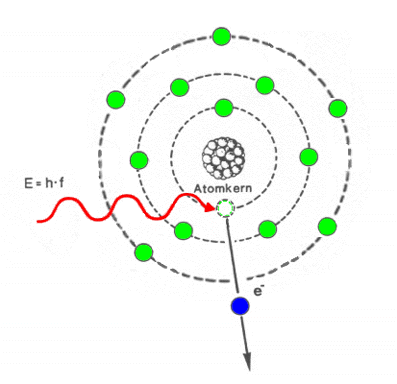
\includegraphics[width=.9\textwidth]{Figures/photoeffekt.png}
            \caption{Schematische Darstellung der Wirkungsweise des
                Photoeffektes.\cite{bib:Photoeffekt}}
            \label{fig:Photoeffekt}
          \end{minipage}\quad
          \begin{minipage}{0.48\textwidth}
            \centering
            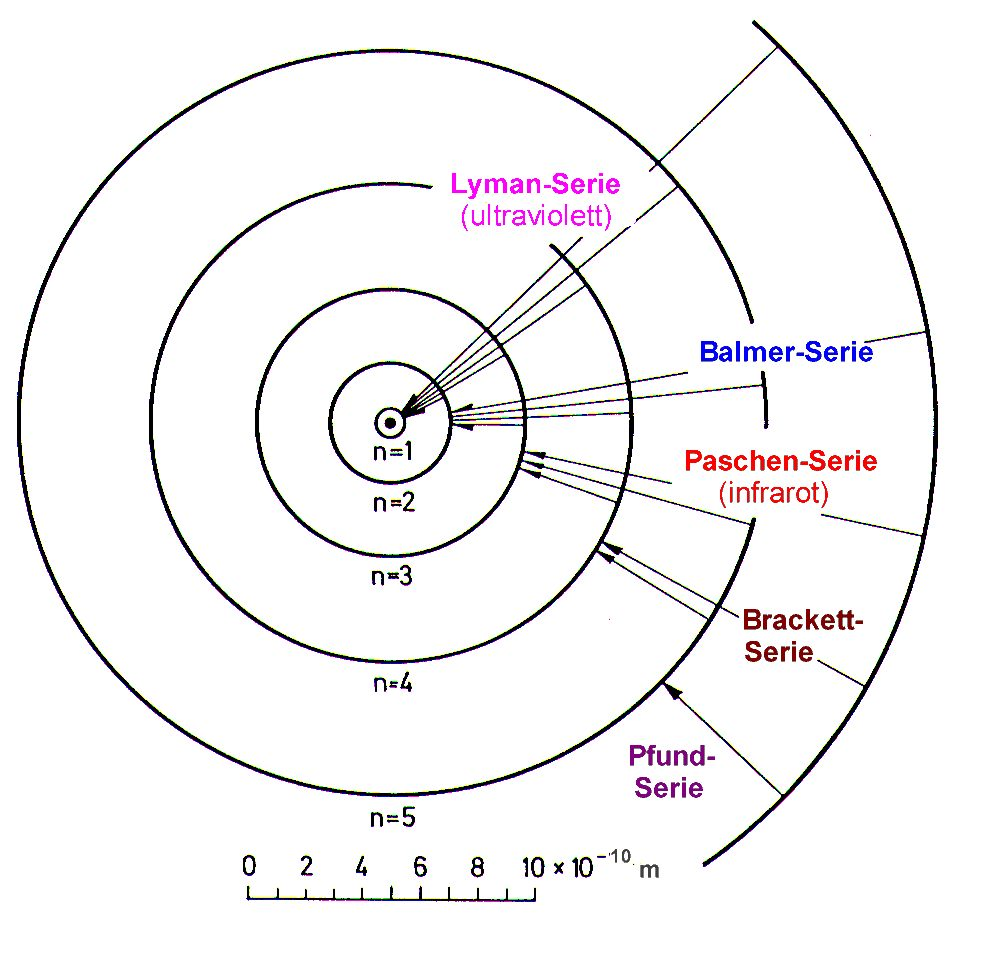
\includegraphics[width=.9\textwidth]
                {Figures/BohrschesAtommodellSerien.png}
            \caption{Bohrsches Atommodell zusammen mit den Übergangsserien.
                \cite{bib:BohrschesAtommodellSerien}}
            \label{fig:BohrschesAtommodellSerien}
          \end{minipage}
        \end{figure}
       
      \end{subsection}
      %%%%%%%%%%%%%%%%%%%%%%%%%%%%%%%%%%%%%%%%
     
     
     
      %%%%%%%%%%%%%%%%%%%%%%%%%%%%%%%%%%%%%%%%
      %%%%%%%%%%%%%%%%%%%%%%%%%%%%%%%%%%%%%%%%
      %%%%%%%%%%%%%%%%%%%%%%%%%%%%%%%%%%%%%%%%
      \begin{subsection}{Photozelle}
        \label{chp:TheoriePhotoelektrischesWirkungsquantumPhotozelle}
        In diesem Versuch wird der Photoeffekt u.A. dafür genutzt um Elektronen
        aus einer Metallplatte heraus zu lösen. Dabei trifft Das Licht einer
        Quecksilberdampflampe mit einer ionisierenden Wellenlänge auf eine
        negativ geladene Metallplatte. Um ein Elektron aus der Oberfläche zu
        lösen muss die spezifische Austrittsarbeit des verwendeten Metalls
        erreicht werden. Aus der Austrittsarbeit ergibt sich mithilfe von
        \cref{eq:Grenzfrequenz} die sog. \textit{Grenzfrequenz}.
        \begin{equation}
          \label{eq:Grenzfrequenz}
          \nu_{0}=\frac{W_{A}}{h}
        \end{equation}
        Die ausgelösten Elektronen können anschließend in der Photozelle
        detektiert werden. Aufgebaut ist die Photozelle aus einem evakuierten
        Gehäuse in dem eine Metallplatte als Kathode angebracht ist. Auf der
        gegenüber liegenden Seite innerhalb des Gehäuses ist ein dünner
        Ringdraht als Anode angeschlossen. An Anode und Kathode kann nun eine
        Spannung angelegt werden um die ausgelösten Elektronen einem Potential
        auszusetzen. Wird nun Spannung erhöht, werden die Elektronen zur Anode
        hin beschleunigt und können als Strom mit einem Amperemeter gemessen
        werden. Wird die Spannung umgepolt, so werden die Elektronen zurück
        auf die Metallplatte beschleunigt und der Anodenstrom verringert sich.
        So kann man die kinetische Energie der ausgelösten Elektronen finden
        indem man die Grenzspannung bestimmt, bei der kein Anodenstrom mehr
        gemessen werden kann. Die maximale kinetische Energie ergibt sich dann
        aus der Differenz der Energie des Photons und der Austrittsarbeit mit
        \cref{eq:Ekin}.
        \begin{equation}
          \label{eq:Ekin}
          E_{kin}=eU_{0}=h\nu-W_{A}
        \end{equation}
       
        \begin{figure}[b]
          \begin{center}
            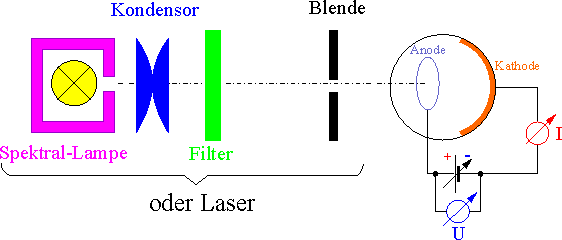
\includegraphics[width=.8\textwidth]
                {Figures/photozelle_mit_aufbau.png}
            \caption{Schematischer Aufbau einer Photozelle. 
                \cite{bib:PhotozelleAufbau}}
            \label{fig:PhotozelleAufbau}
          \end{center}
        \end{figure}

        Um möglichst genaue Messwerte zu erhalten werden Anode und Kathode aus
        Materialien mit unterschiedlichen Ionisierungsenergien verwendet.
        Dadurch kann es vermieden werden, dass der Anodenstrom durch
        Elektronen verfälscht wird, die aus der Anode selbst gelöst wurden.
        Die Verbindung unterschiedlicher Materialien bringt allerdings den
        Nachteil mit sich, dass zwischen ihnen ein sog.
        \textit{Kontaktpotential} entsteht. Dieses Kontaktpotential entsteht,
        da sich die Potentiale (oder Fermi-Niveaus) beider Kontakte im
        Gleichgewicht befinden müssen. Daher kommt zu dieser Gleichung noch
        eine Korrektur für das Kontaktpotential zwischen den Materialien hinzu
        die in \cref{eq:KontaktpotentialKorrektur} gegeben ist.
        \begin{equation}
          \label{eq:KontaktpotentialKorrektur}
          W_{K}^{12}=\left|W_{A}^{1}-W_{A}^{2}\right|
        \end{equation}
        Daraus ergibt sich somit die Kontaktpotential korrigierte Formel für
        die kinetische Energie \cref{eq:EkinKontaktpotential}.
        \begin{equation}
          \label{eq:EkinKontaktpotential}
          E_{kin}=eU_{0}-W_{K}=h\nu-W_{A}-W_{K}
        \end{equation}
       
        \todo[inline]{Sind alle Formel richtig?}
       
      \end{subsection}
      %%%%%%%%%%%%%%%%%%%%%%%%%%%%%%%%%%%%%%%%
     
    \end{section}
    %%%%%%%%%%%%%%%%%%%%%%%%%%%%%%
   
   
   
    %%%%%%%%%%%%%%%%%%%%%%%%%%%%%%
    %%%%%%%%%%%%%%%%%%%%%%%%%%%%%%
    %%%%%%%%%%%%%%%%%%%%%%%%%%%%%%
    \begin{section}{Bohrsches Atommodell und Balmer-Serie}
      \label{chp:TheorieBohrBalmerSerie}
     
     
     
      %%%%%%%%%%%%%%%%%%%%%%%%%%%%%%%%%%%%%%%%
      %%%%%%%%%%%%%%%%%%%%%%%%%%%%%%%%%%%%%%%%
      %%%%%%%%%%%%%%%%%%%%%%%%%%%%%%%%%%%%%%%%
      \begin{subsection}{Aufbau des Borschen Atoms}
        \label{chp:TheorieBohrBalmerSerieAufbauAtomhuelle}
        Das Bohrsche Atommodell ist das wohl bekannteste Atommodell. Für sein
        Modell postulierte Bohr $1913$ die folgenden drei Postulate.
        \begin{enumerate}
          \item Elektronen umkreisen den Atomkern auf festen Bahnen.
          \item Das Elektron kann den Kern nur stabil und ohne
              Energieabstrahlung auf bestimmten, diskreten Bahnen mit festen
              Energien umkreisen.
          \item Elektronen können ihre Energie nur durch Emission oder
              Absorption elektromagnetischer Strahlung ändern.
        \end{enumerate}
        Die Radien der diskreten Bahnen dieser Postulate sind mit
        \cref{eq:Bohrradius} und deren Energien mit
        \cref{eq:BohrradiusEnergien}.
        \newline
        \begin{minipage}{.48\textwidth}
          \begin{equation}
            \label{eq:Bohrradius}
            r_{n}=\frac{n^{2}}{Z}a_{0}=\frac{n^{2}h^{2}\epsilon_{0}}
                {\pi\nu Ze^{2}}
          \end{equation}
        \end{minipage}
        \begin{minipage}{.48\textwidth}
          \begin{equation}
            \label{eq:BohrradiusEnergien}
            E_{n}=-R_{y}\frac{Z^{2}}{n^{2}}
          \end{equation}
        \end{minipage}
       
        \todo[inline]{Hier muss noch was weiter gemacht werden. vielleicht
        etwas zu bahnwechseln ueber Absorption und Emission.}
       
      \end{subsection}
      %%%%%%%%%%%%%%%%%%%%%%%%%%%%%%%%%%%%%%%%
     
     
     
      %%%%%%%%%%%%%%%%%%%%%%%%%%%%%%%%%%%%%%%%
      %%%%%%%%%%%%%%%%%%%%%%%%%%%%%%%%%%%%%%%%
      %%%%%%%%%%%%%%%%%%%%%%%%%%%%%%%%%%%%%%%%
      \begin{subsection}{Spektroskopie}
        \label{chp:TheorieBohrBalmerSerieSpektroskopie}
        Unter den Begriff Spektroskopie fasst man verschiedene Verfahren
        zusammen, Energie in ihr Spektrum zerlegen.
        Wir haben es hier mit der Spektroskopie an einem Refelktionsgitter zu
        tun.
        \begin{figure}[b]
          \begin{center}
            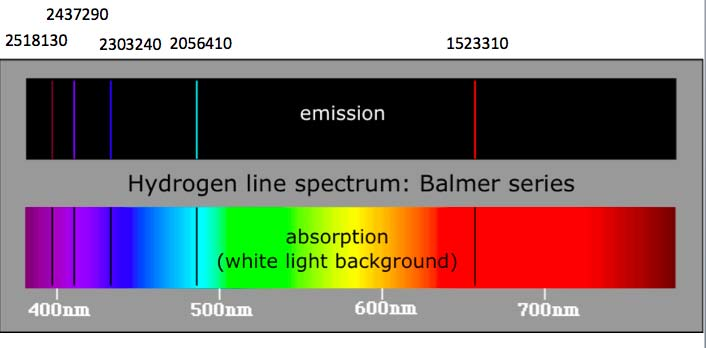
\includegraphics[width=.95\textwidth]
                {Figures/BalmerserieEmissionAbsorption.png}
            \caption{Emissions- und Absorptionslinien der Balmer Übergänge im
                Wasserstoff Atom.
                \cite{bib:BalmerserieEmissionAbsorption}}
            \label{fig:BalmerserieEmissionAbsorption}
          \end{center}
        \end{figure}
        Zur späteren Bestimmung der Gitterkonstante $g$ nutzen wir die
        Gittergleichung:
        \begin{equation}
          \label{eq:Gittergleichung}
          g(\sin(\alpha)+\sin(\beta))=m\lambda
        \end{equation}
       
        \begin{figure}[htbp]
          \begin{center}
            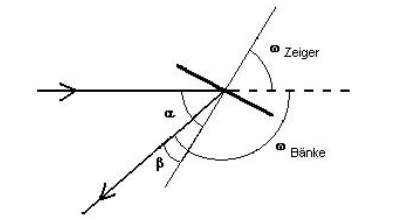
\includegraphics[width=.8\textwidth]{Figures/Gitteraufbau.png}
            \caption{Schematische Darstellung des Reflektionsgitteraufbaus.
                \cite{bib:LDDidactic}}
            \label{fig:Gitteraufbau}
          \end{center}
        \end{figure}
       
        Es werden die Emissionspektren der Quecksilberdampflampe und der Balmer
        Lampe hiermit sichtbar gemacht.
     
      \end{subsection}
      %%%%%%%%%%%%%%%%%%%%%%%%%%%%%%%%%%%%%%%%
     
     
     
      %%%%%%%%%%%%%%%%%%%%%%%%%%%%%%%%%%%%%%%%
      %%%%%%%%%%%%%%%%%%%%%%%%%%%%%%%%%%%%%%%%
      %%%%%%%%%%%%%%%%%%%%%%%%%%%%%%%%%%%%%%%%
      \begin{subsection}{Linienbreite}
        \label{chp:TheorieBohrBalmerSerieLinienbreite}
        Ein wichtiger Punkt bei der Spektroskopie ist die Linienbreite. Es gibt
        verschiedene Effekte, welche die Linienbreite beeinflussen. Die
        natürliche Linienbreite, minimale Breite der Spektrallinie, tritt
        sogar bei einem völlig isolierten Atom. Sie entsteht auf Grund der
        endlichen Strahlungsdauer des Atoms. Hierdurch kommt es zu einer
        Energie-Zeitunschärfe, in der Form einer Resonazkurve. Zusätzlich zu
        der natürlichen Linienbreite gibt es die Dopplerverbreiterung, welche
        durch die Summe  der Bewegung der einzelnen Teilchen in
        unterschiedliche Raumrichtungen entsteht. Bei höheren Temperaturen
        verstärkt sich dieser Effekt, durch die steigende mittlere
        Geschwindigkeit der Teilchen. Die Stoßverbreiterung bewirkt bei
        benachbarten Atomen eine Verschiebung der Energieniveaus. Durch Stöße
        wird die Lebensdauer eines angeregten Zustandes verkürzt, sodass die
        Energie unschärfer wird.
       
        \todo[inline]{formel}
       
      \end{subsection}
      %%%%%%%%%%%%%%%%%%%%%%%%%%%%%%%%%%%%%%%%
     
    \end{section}
    %%%%%%%%%%%%%%%%%%%%%%%%%%%%%%

  \end{chapter}
  %%%%%%%%%%%%%%%%%%%%
         
         
         
  %%%%%%%%%%%%%%%%%%%%
  %%%%%%%%%%%%%%%%%%%%
  %%%%%%%%%%%%%%%%%%%%
  \begin{chapter}{Erster Versuchsteil - Photoeffekt}
    \label{chp:Photoeffekt}
   
   
   
    %%%%%%%%%%%%%%%%%%%%%%%%%%%%%%
    %%%%%%%%%%%%%%%%%%%%%%%%%%%%%%
    %%%%%%%%%%%%%%%%%%%%%%%%%%%%%%
    \begin{section}{Aufbau und Justage}
      \label{chp:photoeffekt:sec:AufbauJustage}
      Wie in der Skizze zu sehen besteht der Aufbau aus einer Hg Lampe, einer
      Blende, einer Linse, dem Filterrad und der Photozelle. Man nutzt eine Hg
      Lampe, da diese bereits ein diskretes Spektrum hat, so dass Filter, die
      einige Nanometer um dem Bereichen der Emissinoslinien liegen,
      ausreichend sind um einen genügend scharfen Wellenlängen bereich zu
      nutzen. Bei dem Aufbau ist wichtig das alle Bauteile so positioniert
      sind, dass die in der Photozelle befindliche Kathode mit Licht
      verschiedener Frequenzen beleuchtet wird. Zunächst ist zu beachten das
      die Bauteile in der oben genannten Reinfolge auf der gleichen höhe
      angeordnet sind. Hierzu wir die Hg Lampe angestellt, die Schutzkappe der
      Photozelle entfernt und das Filterrad auf $\lambda =
      \SI{578}{\nano\meter}$ gestellt. Nun schließt man die Irisblend soweit,
      dass zwar ein Punkt auf der Kathode erscheint, aber die Ringanode nicht
      beleuchtet wird und stellt diesen Punkt mit Hilfe der Linse scharf.
      Zuletzt wird die Schutzkappe wieder über die Photozelle gestülpt und so
      ausgerichtet, dass das Licht durch das Streulicht begrenzende Rohr
      Weiterhin auf die Kathode fällt.
      \begin{figure}[htbp]
        \begin{center}
          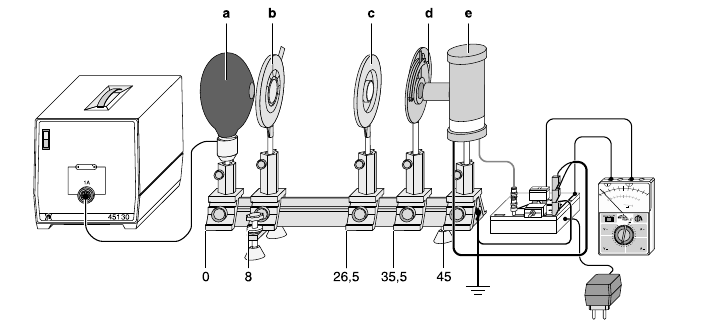
\includegraphics[width=.9\textwidth]{Figures/Planckaufbau.png}
          \caption{Versuchsaufbau auf der Optischen Bank. \textbf{a}:
              Hg-Hochdrucklampe, \textbf{b}: Irisblende,  \textbf{c}: Linse
              f=100mm, \textbf{d}: Frequenz-Filterrad, \textbf{e}: Photozelle.
              Positionsangaben in \textit{cm}. \cite{bib:LDDidactic}}
          \label{fig:Planckaufbau}
        \end{center}
      \end{figure}
      Nach der Jusiterung des Aufbaus ist es wichtig die Fotozelle richtig an
      zu schließen. Wir wollen zwischen Anode und Kathode ein variierbares
      Gegenfeld haben, um die ausgelösten Elektronen auszubremsen und darüber
      deren Energie zu bestimmen. Hierfür schließt man die Anode an den
      negativen Ausgang eines Spannungsteilers angeschlossen und die Kathode
      an den Postiven, welcher auf Masse gezogen wird. Ein Netzgerät mit bis
      zu $\SI{12}{\volt}$ liegt an den Spanungsteiler an, zwischen dessen
      Ausgängen ein Spannungsmessgerät geschaltet ist.
     
    \end{section}
    %%%%%%%%%%%%%%%%%%%%%%%%%%%%%
   
   
   
    %%%%%%%%%%%%%%%%%%%%%%%%%%%%%
    %%%%%%%%%%%%%%%%%%%%%%%%%%%%%
    %%%%%%%%%%%%%%%%%%%%%%%%%%%%%
    \begin{section}{Durchführung}
      \label{chp:Aufbau:sec:ERSTERTEIL:subsec:UNTERTEIL}
      Wir beginnen die Durchführung, indem wir das Filterrad auf den
      kurzwelligsten Filter stellen, an dem Netzgeräte die Gegenspannung hoch
      drehen, bis kein Photostrom mehr fließt und uns aus der größe der
      Spannung überlegen wie der Spannungsteile zusammen gestellt werden soll.
      Wir haben aus den vorhanenden Wiederständen (zwei mal $\SI{100}{\ohm}$,
      und je einmal $\SI{220}{\ohm}$ und $\SI{330}{\ohm}$) ein eine
      Spannungsteilerschaltung mit einem Verhältnis von $\frac{100}{330}$
      gewählt. Nun sollen für die verschiedenen Filter jeweils zwei mal die
      Kennlinien aufgenommen werden.
      %Hierzu ermittelt man zuerst den kleinst möglichen Strom, unser $I_0$
      Um die Kennlinie zu bestimmen beginnt man bei $U=\SI{0}{\volt}$ und
      erhöht langsam die Spannung, bis $I=\SI{0}{\ampere}$, also bis sich die
      Werte für den Strom nicht mehr ändern. An dieser Stelle sind wir
      zunächst jeden Filter einmal durchgegangen. Vor dem zweiten Durchgang
      haben wir festgestellt, dass die Schutzkappe verrutscht ist, wodurch die
      Intensität, welche die Kathode erreicht hat mit der Zeit langsam
      abgeschwächt wurde. Um das im nächsten Durchgang zu vermeiden haben wir
      die Schutzkappe erneut ausgerichtet und mit Klebeband fixiert. Hierdurch
      ist es zu einer großen Intesitätsdifferenz zwischen den beide
      aufgenommenen Kennlinien gekommen. Im Anschluss wird für die Wellenlänge
      $\lambda = \SI{365}{\nano\meter}$ die Intesität deutlich vergrößert und
      erneut eine Kennlinie aufgenommen. 

    \end{section}
    %%%%%%%%%%%%%%%%%%%%%%%%%%%%%
   
   
   
    %%%%%%%%%%%%%%%%%%%%%%%%%%%%%%
    %%%%%%%%%%%%%%%%%%%%%%%%%%%%%%
    %%%%%%%%%%%%%%%%%%%%%%%%%%%%%%
    \begin{section}{Auswertung des ersten Versuchstages}
      \label{chp:Photoeffekt:sec:Auswertung}
      \begin{figure}[b!]
        \begin{center}
          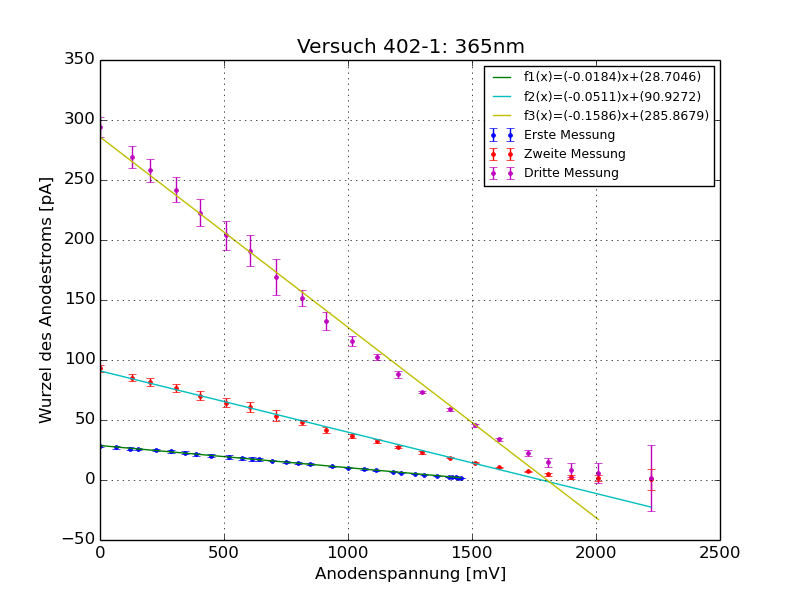
\includegraphics[width=\textwidth]{Figures/Versuch402_1_365.png}
          \caption{Messdaten für drei unterschiedliche Intensitäten.
              Wellenlänge: \SI{365}{\nano\meter}}
          \label{fig:Versuch402_1_365}
        \end{center}
      \end{figure}
      Um das Plancksche Wirkungsquantum zu bestimmen müssen bei jeder Messung
      die jeweilige Grenzspannung bestimmt werden. Diese können sehr einfach
      aus den Graphen abgelesen werden. Die Grenzspannung findet sich für jede
      Wellenlänge als X-Achsen Schnittpunkt, da die Grenzspannung jene ist,
      bei der der Anodenstrom verschwindet. Die Messung der niedrigsten
      Wellenlänge haben wir für drei unterschiedliche Intensitäten vorgenommen
      um zu zeigen, dass die Granzspannung unabhängig der Intensität ist und
      ausschließich durch die Wellenlänge bestimmt wird. In
      \cref{fig:Versuch402_1_365} kann man gut erkennen, dass diese
      Abhängigkeit tatsächlich zutrifft. In
      \crefrange{fig:Versuch402_1_405}{fig:Versuch402_1_578} sind alle
      Messdaten der anderen Wellenlängen ebenfalls in unterschiedlichen
      Intensitäten dargestellt. Um aus diesen Messwerten tatsächlich das
      Plancksche Wirkungsquantum zu bestimmen müssen die verschiedenen
      Grenzspannungen gegen die zugehörige Frequenz der Photonen aufgetragen
      und eine Gerade an die Messwerte angepasst werden. Aus der
      Resultierenden Steigung lässt sich mit \cref{eq:Ekin} und der Elektronen
      Ladung das Plancksche Wirkungsquantum berechnen. Aus unseren Messungen
      erhalten wir eine Steigung der Grenzspannungen von
      $(3.79\pm0.10)\times\SI{e-15}{\volt\per\hertz}$. Daraus berechnet sich 
      für unsere Messungen ein Wirkungsquantum 
      $h=(6.08 \pm 0.16)\times\SI{e-34}{\joule\second}$.
     
      \begin{figure}[htbp]
        \centering
        \begin{minipage}{0.48\textwidth}
          \centering
          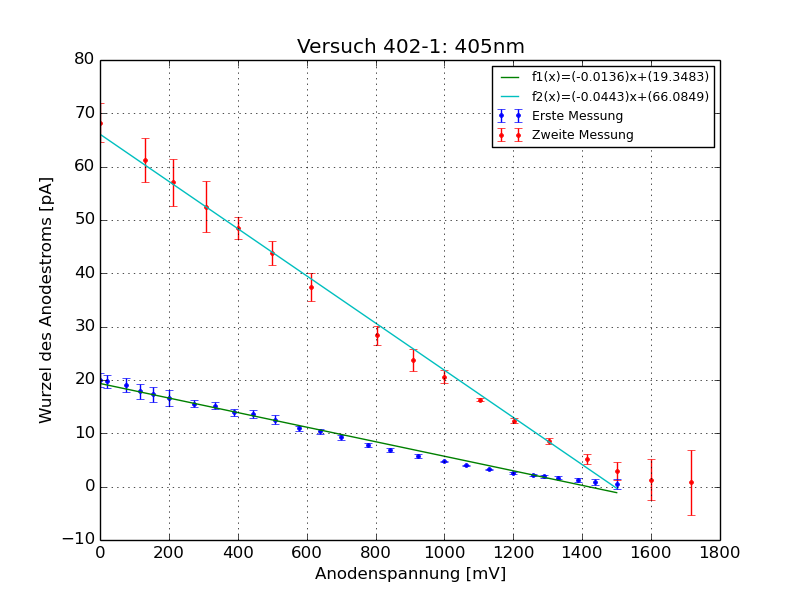
\includegraphics[width=\textwidth]{Figures/Versuch402_1_405.png}
          \caption{Messdaten für zwei unterschiedliche Intensitäten.
              Wellenlänge: \SI{405}{\nano\meter}}
          \label{fig:Versuch402_1_405}
        \end{minipage}\quad
        \begin{minipage}{0.48\textwidth}
          \centering
          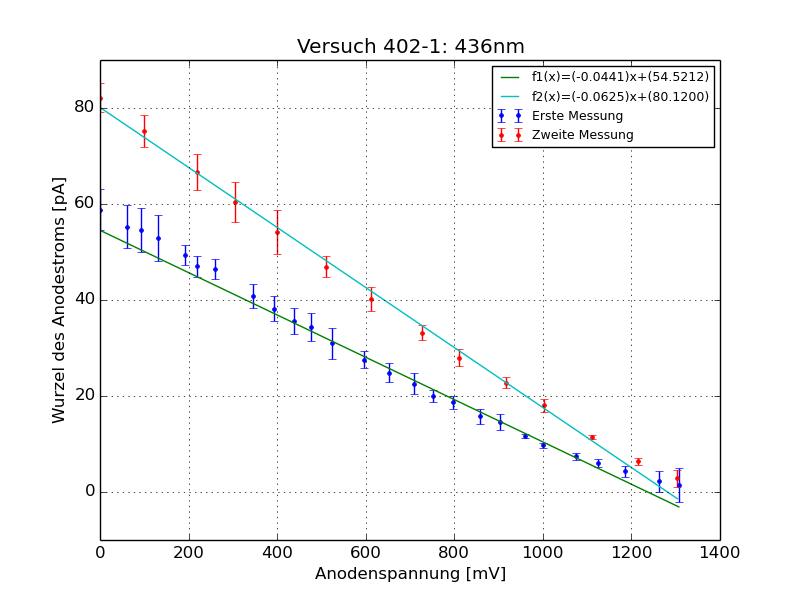
\includegraphics[width=\textwidth]{Figures/Versuch402_1_436.png}
          \caption{Messdaten für zwei unterschiedliche Intensitäten.
              Wellenlänge: \SI{436}{\nano\meter}}
          \label{fig:Versuch402_1_436}
        \end{minipage}
        \begin{minipage}{0.48\textwidth}
          \centering
          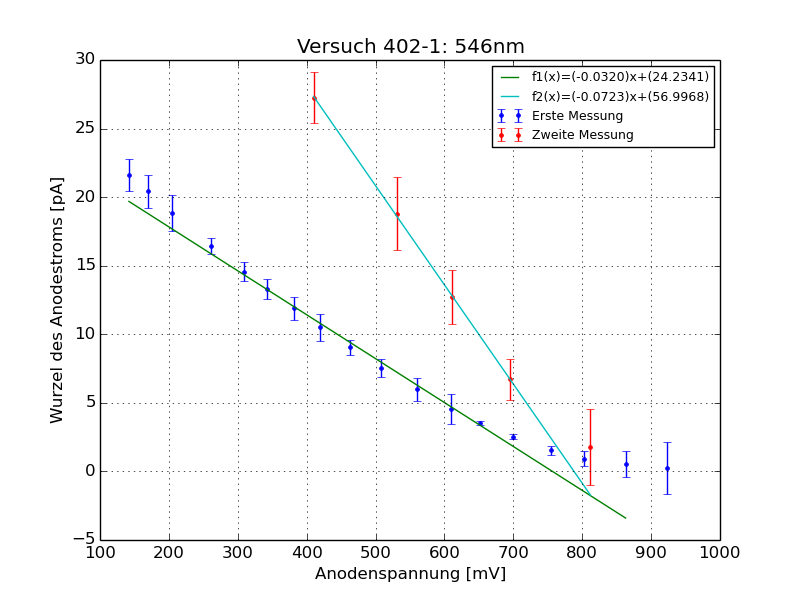
\includegraphics[width=\textwidth]{Figures/Versuch402_1_546.png}
          \caption{Messdaten für zwei unterschiedliche Intensitäten.
              Wellenlänge: \SI{546}{\nano\meter}}
          \label{fig:Versuch402_1_546}
        \end{minipage}\quad
        \begin{minipage}{0.48\textwidth}
          \centering
          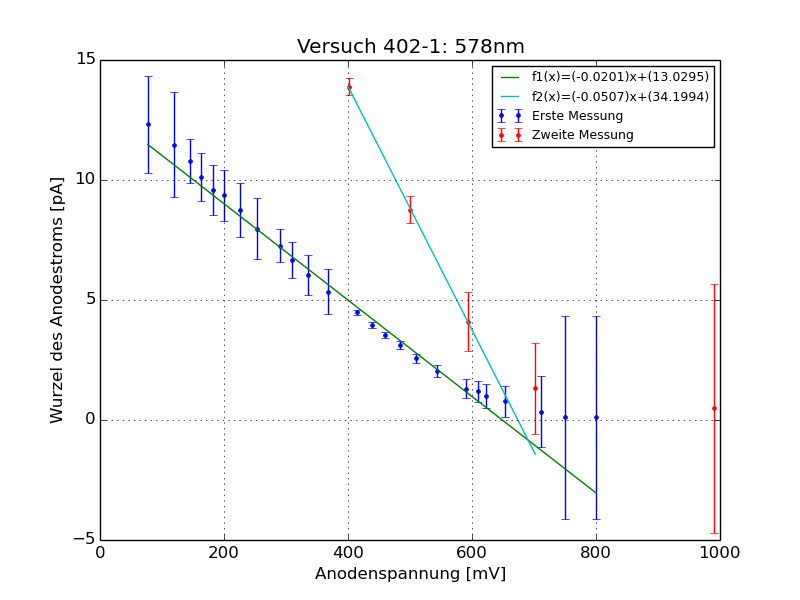
\includegraphics[width=\textwidth]{Figures/Versuch402_1_578.png}
          \caption{Messdaten für zwei unterschiedliche Intensitäten.
              Wellenlänge: \SI{578}{\nano\meter}}
          \label{fig:Versuch402_1_578}
        \end{minipage}
      \end{figure}
      
      Aus dem Y-Achsen Schnittpunk der angepassten Geraden in 
      \cref{fig:Versuch402_1_PlanckschesWirkungsquant} und \cref{eq:Ekin} 
      lässt sich außerdem noch eine Aussage über die Größe des Störterms aus 
      \cref{eq:Ekin} treffen. Der Schnittpunk mit der Y-Achse entspricht 
      hierbei der Summe von Auslösearbeit und Kontaktpotential in 
      $\SI{}{\electronvolt}$. Aus den Parametern der angepassten Geraden 
      beläuft sich diese Summe auf 
      $W_{A}+W_{K}=(1.3759\pm0.0675)\SI{}{\electronvolt}$. Da die verwendeten 
      Materialien der Photozelle nicht bekannt sind kann diese Summe leider 
      nicht weiter differenziert werden.
      
      \begin{figure}[ht]
        \begin{center}
          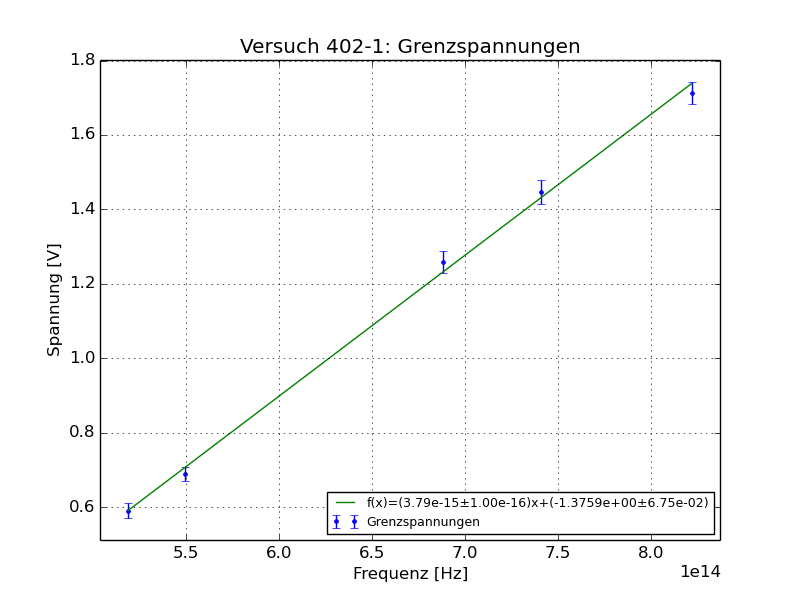
\includegraphics[width=\textwidth]
          {Figures/Versuch402_1_PlanckschesWirkungsquant.png}
          \caption{Graphische Darstellung aller Grenzspannungen zur Bestimmung
              des Planckschen Wirkungsquantum.}
          \label{fig:Versuch402_1_PlanckschesWirkungsquant}
        \end{center}
      \end{figure}
     
    \end{section}
    %%%%%%%%%%%%%%%%%%%%%%%%%%%%%%
   
   
   
    %%%%%%%%%%%%%%%%%%%%%%%%%%%%%%
    %%%%%%%%%%%%%%%%%%%%%%%%%%%%%%
    %%%%%%%%%%%%%%%%%%%%%%%%%%%%%%
    \begin{section}{Fazit - Photoeffekt}
      \label{chp:Photoeffekt:sec:Fazit}
      Zusammenfassend können wir nicht sagen, dass unsere Messung eine
      tatsächlich genaue Bestimmung des Planckschen Wirkungsquantum lieferte da
      die Abweichung zum Literaturwert von
      $h_{Lit}=\SI{6.62607e-34}{\joule\second}$ leider nicht zu leugnen sind.
      Selbst mit dem Fehler unserer Messung liegt der Literaturwert nicht in
      unseren Fehlergrenzen von
      $h=(6.08 \pm 0.16)\times\SI{e-34}{\joule\second}$ 
      Über die Ursachen dieser doch relativ großen Abweichung können wir zu 
      diesem Zeitpunkt leider nur spekulieren. Womöglich liegt es an der 
      Konstruktionsweise des Experimentes an sich, dass keine genauere Messung
      möglich ist. Diese Möglichkeit erscheint uns hier noch als die 
      wahrscheinlichste, da die Herausgeber des Experimentes 
      \textit{LD-Didactics} in ihrer eigenen Durchführung des Versuches selbst
      lediglich auf ein $h_{LD}=\SI{6.1e-34}{\joule\second}$ ohne Fehlerangabe
      kommen.\cite{bib:LDDidactic} \\
      Dieser Wert hingegen liegt sehr gut innerhalb unseres Fehlerbereiches.
      Somit können wir abschließen, dass wir diesen Versuch mit für uns
      akzeptabler genauigkeit durchgeführt haben. Das Experiment selbst 
      hingegen scheint noch unberücksichtigte Fehlerquellen zu beinhalten
      die wir leider mit einbeziehen konnten.\\
      Alle berechneten Fehler resultieren hierbei aus der Fehlerfortpflanzung.
      
      \todo[inline]{sollten wir hier noch etwas zusammenfassendes zu der 
          Ausloesearbeit und dem Kontaktpotential schreiben?}
      
    \end{section}
    %%%%%%%%%%%%%%%%%%%%%%%%%%%%%%
   
  \end{chapter}
  %%%%%%%%%%%%%%%%%%%%
 
 
 
  %%%%%%%%%%%%%%%%%%%%
  %%%%%%%%%%%%%%%%%%%%
  %%%%%%%%%%%%%%%%%%%%
  \begin{chapter}{Zweiter Versuchsteil - Balmer-Serie}
    \label{chp:Balmer}
 
 
    %%%%%%%%%%%%%%%%%%%%%%%%%%%%%%
    %%%%%%%%%%%%%%%%%%%%%%%%%%%%%%
    %%%%%%%%%%%%%%%%%%%%%%%%%%%%%%
    \begin{section}{Aufbau}
      \label{chp:Balmer:sec:Aufbau}
      Ziel dieses Versuchsteils ist es, dass Spektrum einer
      Wasserstoff-Deuterium-Lampe, die so genannte Balmerserie, zu bestimmen.
      Hierzu nutzen wir ein Rfelexionsgitter, welches zwischen zwei gewinkleten
      Armen einer optischen Bank steht. Der Winkel zwischen beiden Armen kann
      abgelesen werden. Zu Beginn stehen an dem einen Ende der optischen Bank
      eine Hg Lampe und am anderen ein Okular mit Strichskala, um die
      Gitterkonstante zu bestimmen. Im Verlauf des Versuchs wir zuerst die
      Lampe gegen die Wasserstoff-Deuterium-Lampe und später das Okular gegen
      einen CCD-Kamera ausgetauscht. Die gesammt Anordnung ist, wie auch auf
      dem Bilder zu sehen, Balmer-Lampe, Linse mit einer Brennweite von
      $f=\SI{50}{\milli\meter}$, ein verstellbarer Spalt, ein
      Projektionsojektiv mit $f=\SI{150}{\milli\meter}$, das
      Refelxionsgitter,eine weitere Linse mit $f=\SI{300}{\milli\meter}$ und
      zu guter letztdas Okular, beziehungsweise die CCD-Kamera.
      
      \begin{figure}[h]
        \begin{center}
          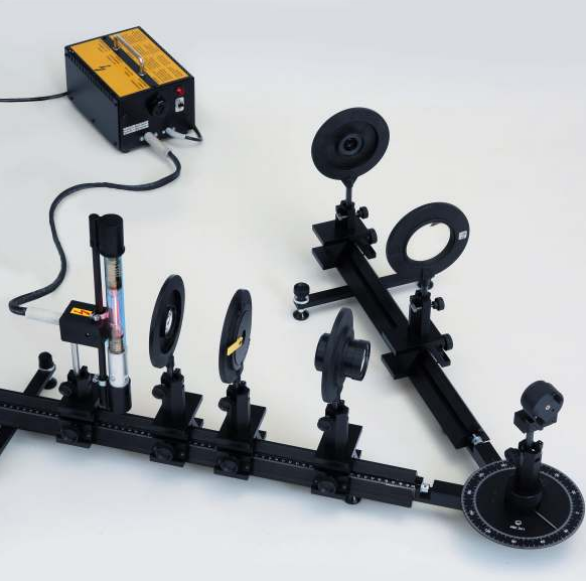
\includegraphics[width=.7\textwidth]{Figures/Balmeraufbau.png}
          \caption{Versuchsaufbau zur Messung der Balmer-Serie.
              \cite{bib:LDDidactic}}
          \label{fig:BalmerAufbau}
        \end{center}
      \end{figure}
      
    \end{section}
    %%%%%%%%%%%%%%%%%%%%%%%%%%%%%%
   
   
   
    %%%%%%%%%%%%%%%%%%%%%%%%%%%%%%
    %%%%%%%%%%%%%%%%%%%%%%%%%%%%%%
    %%%%%%%%%%%%%%%%%%%%%%%%%%%%%%
    \begin{section}{Justierung und Durchführung}
      \label{chp:Balmer:sec:JusitierungDurchfuehrung}
     
     
     
      %%%%%%%%%%%%%%%%%%%%%%%%%%%%%%%%%%%%%%%%
      %%%%%%%%%%%%%%%%%%%%%%%%%%%%%%%%%%%%%%%%
      %%%%%%%%%%%%%%%%%%%%%%%%%%%%%%%%%%%%%%%%
      \begin{subsection}{Justierung}
        \label{chp:Balmer:sec:JusitierungDurchfuehrung:subsec:Justierung}
        Zunächst ist der Anfangsaufbau mit der Hg Lampe zu Justieren. Nach
        einsetzen der Lampe wird die erste Linse ($f=\SI{50}{\milli\meter}$)
        so eingesetzt, das sie die Lichtquelle auf die schrägen Flanken des
        senkrecht stehenden Splates abbildet. Als nächstes wird das Objektiv
        eingesetzt und mit Hilfe der Autokollimation justiert. Das lässt sich
        realisieren, indem man das Gitter so dreht, dass die Reflektion erneut
        durch das Objektiv fällt und somit den Spalt neben den Spalt abbildet.
        Wenn man diese Abbildung des Splates nun scharf stellt, ist diese nach
        dem Objektiv auf Unendlich fokussiert. Nun legen wir die Abbildung des
        Spaltes über dem Spalt und stellen den Winkel zwischen den Armen der
        optischen Bänke auf $\alpha-\beta = \SI{30}{\degree}$. Dieser Winkel
        wird von uns den ganzen Versuch über nicht geändert. Am Ende des
        zweiten Armses wird das Okular so montiert, dass die Skala gut
        abzulesen ist. Um die verschiedenen Spektrallinien auf die Skala
        scharf ab zu bilden stellen man die letzte Linse in den Strahlengang
        und verschiebt diese je nach bedarf. So entsteht ein
        Beobachtungsteleskop.

      \end{subsection}
      %%%%%%%%%%%%%%%%%%%%%%%%%%%%%%%%%%%%%%%%
     
     
     
      %%%%%%%%%%%%%%%%%%%%%%%%%%%%%%%%%%%%%%%%
      %%%%%%%%%%%%%%%%%%%%%%%%%%%%%%%%%%%%%%%%
      %%%%%%%%%%%%%%%%%%%%%%%%%%%%%%%%%%%%%%%%
      \begin{subsection}{Bestimmung der Gitterkonstante}
        \label{chp:Balmer:sec:JusitierungDurchfuehrung:subsec:Gitter}
        Um Gitterkonstante zu bestimmen nehmen wir die Hg Lampe. Diese benutzen
        wir, da sie eine hohe Intesität hat, wodurch die Spektrallinien gut
        sichtbar sind. Außerdem haben kennen wir deren Wellenlängen und können
        so diese den beobachteten Wellenlängen identifizieren um die
        Gitterkonstante zu bestimmen. Wir drehen an der Gittersäule so, um die
        ersten Linien im Okular sichtabr zu machen. Nun stellen wir mit Hilfe
        der $f=\SI{300}{\milli\meter}$ Linse die Linien scharf und notieren
        uns die Farbe und den Gitterwinkel $\omega_G$. So gehen wir vor bis
        wir alle sichtbaren Linien notiert haben. Durch den vergleich mit den
        gegebenen Wellenlängen für Spektrallinien lassen sich so den Winkel
        Wellenlängen zu ordnen.
       
        \begin{table}[htbp]
          \centering
          \footnotesize
          \begin{tabular}{|c|c|c|c|c|c|c|}
            \hline
            Farbe & Wellenlänge [nm] & Winkel & rel. Int. & 
            Linienbreite & Gitter g [nm] & Fehler $\Delta g$ \\ 
                \hline \hline 
            Rot & 690.752 & 66.2 & 1.0 & 0.3 & 458.8 & 3.23 \\ \hline 
            Rot & 671.643 & 65.0 & 1.0 & 0.25 & 453.85 & 3.33 \\ \hline
            Rot & 623.44 & 64.5 & 0.5 & 0.25 & 424.4 & 3.17 \\ \hline
            Gelb & 579.066 & 61.5 & 3.0 & 0.3 & 413.23 & 3.43 \\ \hline
            Gelb & 576.96 & 61.3 & 3.0 & 0.25 & 413.1 & 3.45 \\ \hline 
            Grün & 546.074 & 58.0 & 10.0 & 0.2 & 414.5 & 3.89 \\ \hline
            Türkis & 491.607 & 53.0 & 3.0 & 0.35 & 413.34 & 4.63 \\ \hline
            Blau & 435.833 & 48.3 & 5.0 & 0.5 & 410.92 & 5.47 \\ \hline
            Blau & 434.749 & 48.2 & 2.0 & 0.3 & 410.99 & 5.49 \\ \hline 
            Blau & 433.922 & 48.1 & 2.0 & 0.3 & 411.31 & 5.52 \\ \hline
            Violett & 410.805 & 46.0 & 0.5 & 0.4 & 412.88 & 6.01 \\ \hline
            Violett & 407.783 & 45.7 & 2.0 & 0.4 & 413.45 & 6.09 \\ \hline
            Violett & 404.656 & 45.4 & 4.0 & 0.5 & 413.94 & 6.17 \\ \hline
          \end{tabular}
          \caption{Messreihe zur Bestimmung der Gitterkonstanten mithilfe 
              der Hg-Lampe. Mit einem Ablesefehler auf die Winkel von 
              $\SI{0.5}{\degree}$}
          \label{tab:GitterkonstanteHg}
        \end{table}

      \end{subsection}
      %%%%%%%%%%%%%%%%%%%%%%%%%%%%%%%%%%%%%%%%
     
     
     
      %%%%%%%%%%%%%%%%%%%%%%%%%%%%%%%%%%%%%%%%
      %%%%%%%%%%%%%%%%%%%%%%%%%%%%%%%%%%%%%%%%
      %%%%%%%%%%%%%%%%%%%%%%%%%%%%%%%%%%%%%%%%
      \begin{subsection}{Untersuchung der Balmer-Linie mit einem Okular}
        \label{chp:Balmer:sec:JusitierungDurchfuehrung:subsec:Okular}
        Als nächstes tauschen wir die Hg Lampe durch eine Balmer-Lampe und
        überprüfen die Justierung. Dann suchen wir durch drehen der Gittersäule
        erneut die erste Linie und notieren uns die Farbe, den Winkel und die
        Breite der Linien $d$, welche den Abstand der Aufspaltung der
        Linienbreite representiert. Hierfür ist besonders wichtig die Linen
        auf die Skala scharf zu stellen. Für die anderen Linien wiederholen
        wir dieses Vorgehen.
         
        \begin{table}[htbp]
          \centering
          \footnotesize
          \begin{tabular}{|c|c|c|c|c|c|c|c|}
            \hline
            Farbe & Winkel & rel. Int. & Lin. Breite & $\lambda$ 
                [nm] & Fehler $\Delta \lambda$ & Isotr.Aufsp. 
                $d\lambda_{Iso}$ & $\Delta d\lambda_{Iso}$ \\ \hline \hline 
            Rot & 70.0 & 3.0 & 0.4 & 665.21 & 9.0 & 0.196 & 0.108 \\ \hline 
            Rot & 65.2 & 1.0 & 0.3 & 623.90 & 8.91 & 0.180 & 0.114 \\ \hline 
            Gelb & 61.4 & 0.05 & 0.1 & 588.08 & 8.83 & 0.068 & 0.120 \\ \hline 
            Grün & 57.5 & 0.3 & 0.2 & 548.63 & 8.74 & 0.153 & 0.124 \\ \hline 
            Grün & 56.8 & 0.3 & 0.2 & 541.27 & 8.72 & 0.155 & 0.125 \\ \hline 
            Türkis & 52.5 & 3.0 & 0.3 & 494.36 & 8.62 & 0.259 & 0.130 \\ \hline
            Violett & 47.9 & 0.5 & 0.2 & 441.10 & 8.51 & 0.190 & 0.133 \\ 
                \hline 
            Violett & 47.7 & 1.0 & 0.2 & 438.71 & 8.51 & 0.190 & 0.134 \\ 
                \hline 
            Violett & 45.8 & 0.05 & 0.2 & 415.81 & 8.46 & 0.197 & 0.135 \\ 
                \hline 
          \end{tabular}
          \caption{Messreihe zur Bestimmung der Wellenlängen der Balmer-Serie 
              mithilde der H/D-Lampe. Mit einem Ablesefehler auf die Winkel 
              von $\SI{0.5}{\degree}$}
          \label{tab:BalmerserieOkular}
        \end{table}

      \end{subsection}
      %%%%%%%%%%%%%%%%%%%%%%%%%%%%%%%%%%%%%%%%
     
     
     
      %%%%%%%%%%%%%%%%%%%%%%%%%%%%%%%%%%%%%%%%
      %%%%%%%%%%%%%%%%%%%%%%%%%%%%%%%%%%%%%%%%
      %%%%%%%%%%%%%%%%%%%%%%%%%%%%%%%%%%%%%%%%
      \begin{subsection}{Untersuchung der Balmerlinie mit der CCD-Kamera}
        \label{chp:Balmer:sec:JusitierungDurchfuehrung:subsec:CCD}
        Für den nächsten Versuchteil wird das Okular durch die CCD-Kamera
        ersetzt. Dabei muss dadrauf geachtet werden, dass CCD-Zeile beleuchtet
        wird. Die Kamera wird an den PC angeschlossen und mit Strom versorgt.
        Auf dem PC öffnet man Das Programm VideoCom und wählt die
        Einstellungen aus der Versuchsanleitung. Wir wollen die
        Isotropieaufspaltung messen, also suchen wir nach Ausschlägen, indem
        wir mit der Gittersäule die Winkel ansteuern, die wir zuvor ermittelt
        haben. Sobald auf dem Monitor einer dieser Ausschläge erscheint,
        versuchen wir durch Vergrößerung des Abschnittes, Mittelwertbildung
        der Intesität und verschieben der letzten Linse zwei scharfe getrennte
        Spitzen oder Überlagerungen zu erhalten. Aus den so aufgenommenen
        Messdaten lässt sich die Linienverbreiterung bestimmen.
        
      \begin{figure}[ht!]
        \centering
        \begin{minipage}{0.48\textwidth}
          \centering
          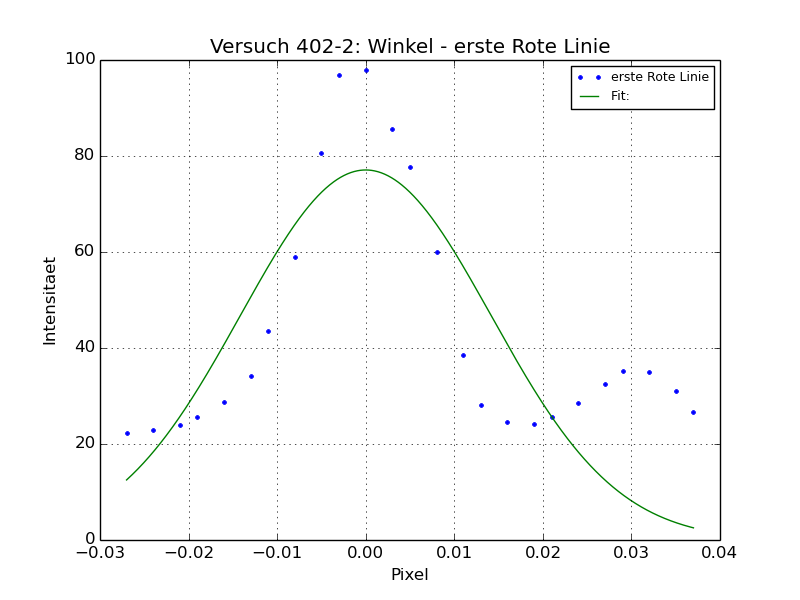
\includegraphics[width=\textwidth]
              {Figures/Versuch402_2_ersteRoteLinie.png}
          \caption{Messdaten der erste rote Linie.}
          \label{fig:Versuch402_2_ersteRoteLinie}
        \end{minipage}\quad
        \begin{minipage}{0.48\textwidth}
          \centering
          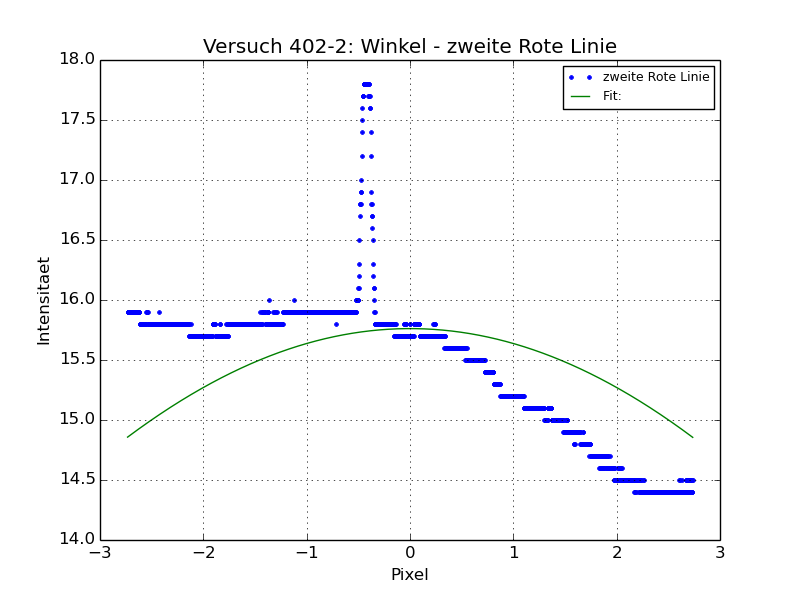
\includegraphics[width=\textwidth]
              {Figures/Versuch402_2_zweiteRoteLinie.png}
          \caption{Messdaten der zweite rote Linie.}
          \label{fig:Versuch402_2_zweiteRoteLinie}
        \end{minipage}
        \begin{minipage}{0.48\textwidth}
          \centering
          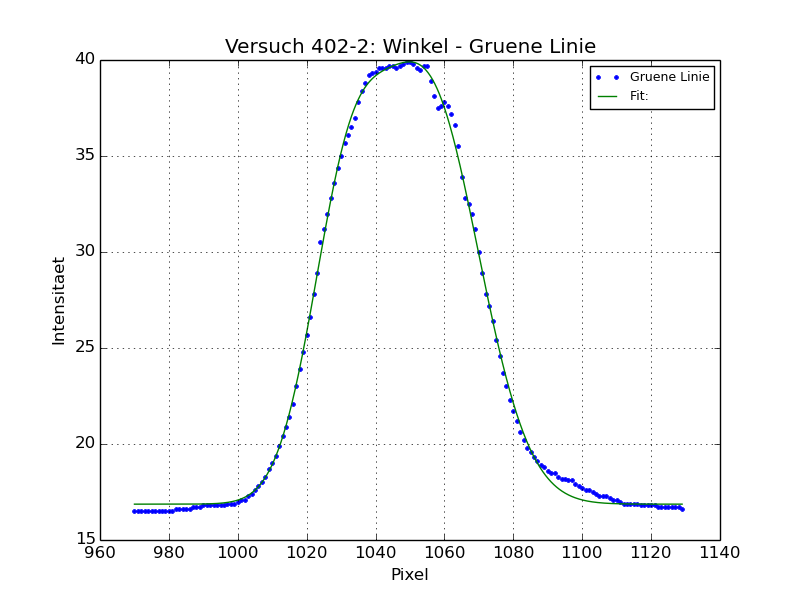
\includegraphics[width=\textwidth]
              {Figures/Versuch402_2_GrueneLinie.png}
          \caption{Messdaten der grüne Linie.}
          \label{fig:Versuch402_2_GrueneLinie}
        \end{minipage}\quad
        \begin{minipage}{0.48\textwidth}
          \centering
          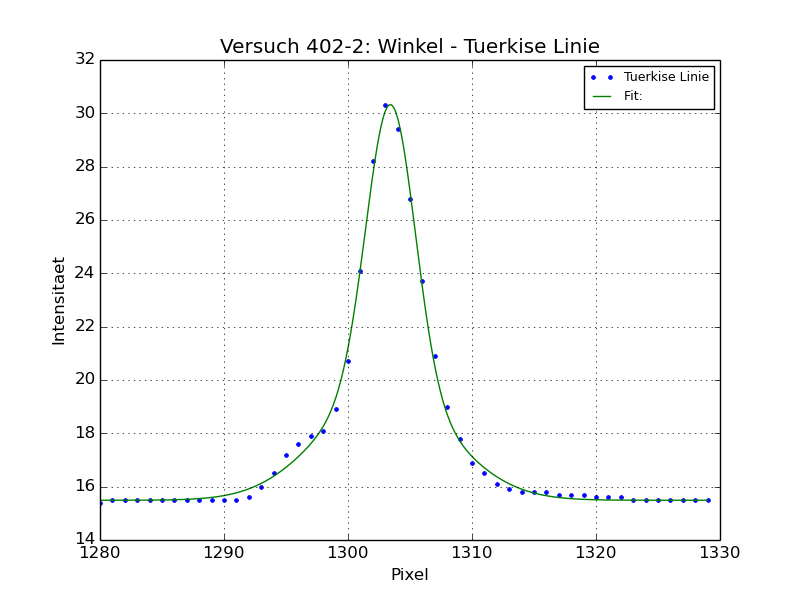
\includegraphics[width=\textwidth]
              {Figures/Versuch402_2_TuerkiseLinie.png}
          \caption{Messdaten der türkise Linie.}
          \label{fig:Versuch402_2_TuerkiseLinie}
        \end{minipage}
        \begin{minipage}{0.48\textwidth}
          \centering
          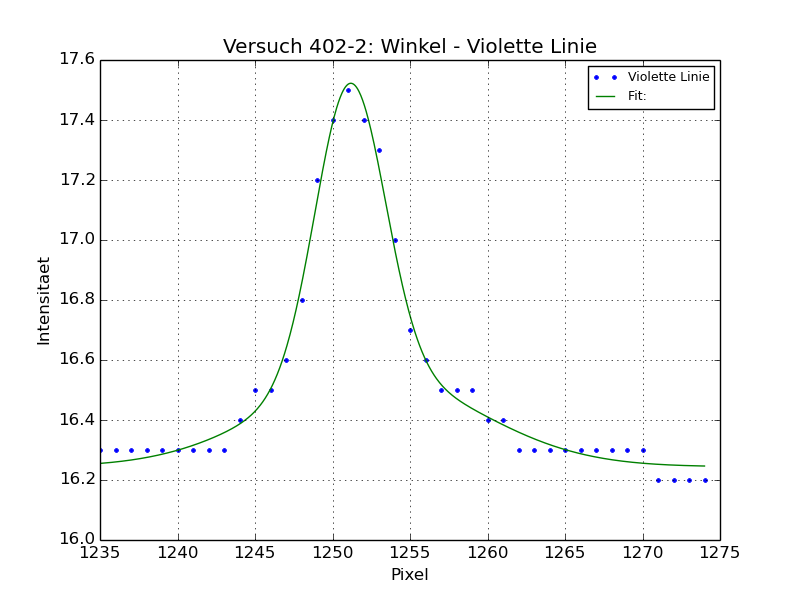
\includegraphics[width=\textwidth]
              {Figures/Versuch402_2_VioletteLinie.png}
          \caption{Messdaten der violette Linie.}
          \label{fig:Versuch402_2_VioletteLinie}
        \end{minipage}\quad
        \begin{minipage}{0.48\textwidth}
          \centering
          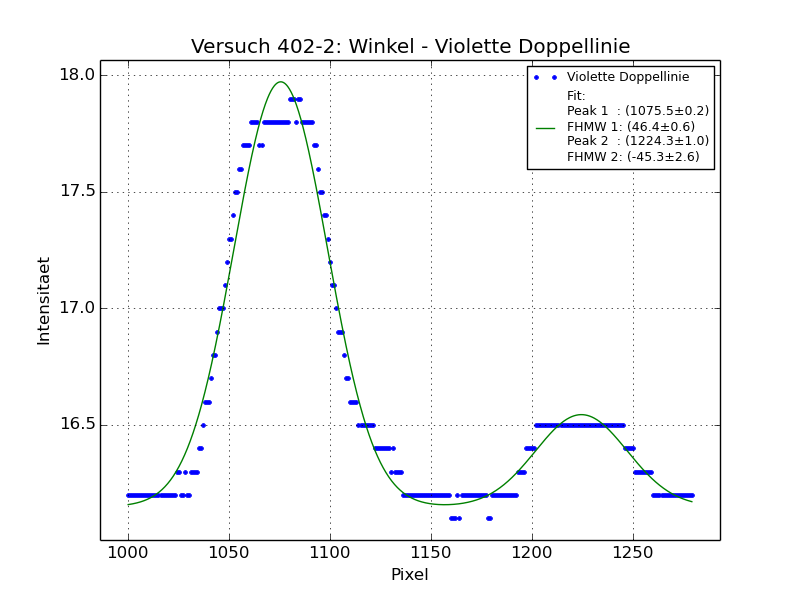
\includegraphics[width=\textwidth]
              {Figures/Versuch402_2_VioletteDoppellinie.png}
          \caption{Messdaten der violetten Doppellinie.}
          \label{fig:Versuch402_2_VioletteDoppellinie}
        \end{minipage}
      \end{figure}

      \end{subsection}
      %%%%%%%%%%%%%%%%%%%%%%%%%%%%%%%%%%%%%%%%

    \end{section}
    %%%%%%%%%%%%%%%%%%%%%%%%%%%%%%


    

    %%%%%%%%%%%%%%%%%%%%%%%%%%%%%%
    %%%%%%%%%%%%%%%%%%%%%%%%%%%%%%
    %%%%%%%%%%%%%%%%%%%%%%%%%%%%%%
    \begin{section}{Auswertung}
      \label{chp:Balmer:sec:Auswertung}
      
      
      
      %%%%%%%%%%%%%%%%%%%%%%%%%%%%%%%%%%%%%%%%
      %%%%%%%%%%%%%%%%%%%%%%%%%%%%%%%%%%%%%%%%
      %%%%%%%%%%%%%%%%%%%%%%%%%%%%%%%%%%%%%%%%
      \begin{subsection}{Bestimmung der Gitterkonstante}
        \label{chp:Balmer:sec:Auswertung:subsec:Gitterkonstante}
        Um die Gitterkonstante aus unseren Messwerten zu bestimmen benutzen 
        wir \cref{eq:Gittergleichung} und formen nach der Gitterkonstanten um.
        Aus den Messwerten und den, in de Versuchsanleitung angegebenen,
        Wellenlänge erhalten wir anschließend die Gitterkonstante
        $g=(420.36 \pm 4.75) \SI{}{\nano\meter}$. Dieses Messergebnis passt 
        mit den angegebenen Fehlergrenzen gut in die Angaben des Herstellers, 
        welcher die Gitterkonstante mit $g_{LD}=\SI{416.67}{\nano\meter}$ 
        angibt.\cite{bib:LDDidactic}
        
      \end{subsection}
      %%%%%%%%%%%%%%%%%%%%%%%%%%%%%%%%%%%%%%%%
      
      
      
      %%%%%%%%%%%%%%%%%%%%%%%%%%%%%%%%%%%%%%%%
      %%%%%%%%%%%%%%%%%%%%%%%%%%%%%%%%%%%%%%%%
      %%%%%%%%%%%%%%%%%%%%%%%%%%%%%%%%%%%%%%%%
      \begin{subsection}{Bestimmung der Balmer-Linien mit dem Okular}
        \label{chp:Balmer:sec:Auswertung:subsec:Okular}
        Nachdem wir nun die Gitterkonstante bestimmt 
        haben können wir aus den Beobachtungen der Balmer-Linien der 
        H/D-Lampe deren Wellenlängen berechnen. Dazu benutzen wir wieder 
        \cref{eq:Gittergleichung} und erhalten so die jeweiligen Wellenlängen. 
        Die Ergebnisse dieser Rechnung sind in \cref{tab:BalmerserieOkular} 
        festgehalten. \\
        Außerdem haben wir bei unseren Messungen die Aufspaltung der einzelnen 
        Linien mit einer, im Okular angebrachten Messskala beobachtet. Aus der 
        Linienbreite lässt sich mit \cref{eq:Isotropieaufspaltung} die 
        Isotropieaufspaltung der Balmerlinien berechnen.
        \begin{equation}
          \label{eq:Isotropieaufspaltung}
          \Delta\lambda=\frac{dgcos(\beta)}{f}
        \end{equation}
        Wobei in \cref{eq:Isotropieaufspaltung} \textbf{d} die abgelesene 
        Breite der Linie im Okular (in $\SI{}{\milli\meter}$) und \textbf{f} 
        die Brennweite der Fokuslinse vor dem Okular (ebenfalls in 
        $\SI{}{\milli\meter}$) ist.
        
      \end{subsection}
      %%%%%%%%%%%%%%%%%%%%%%%%%%%%%%%%%%%%%%%%
      
      
      
      %%%%%%%%%%%%%%%%%%%%%%%%%%%%%%%%%%%%%%%%
      %%%%%%%%%%%%%%%%%%%%%%%%%%%%%%%%%%%%%%%%
      %%%%%%%%%%%%%%%%%%%%%%%%%%%%%%%%%%%%%%%%
      \begin{subsection}{Bestimmung des Planckschen Wirkungsquantum mit der
          CCD-Kamera}
        \label{chp:Balmer:sec:Auswertung:subsec:CCD}
        Aus den angepassten Gauss-Kurven lässt sich nun die 
        Isotropieaufspaltung bestimmen. Leider erhalten wir bei unseren 
        Rechnungen dazu nur Ergebnisse der Isotropieaufspaltung im Bereich von
        einigen Nanometern bis hin zu über $100nm$. Diese Werte sind 
        physikalisch natürlich nicht sinnvoll, sodass wir auch nach langer
        Fehlersuche und merfach wiederholtem, neuen erstellen der Rechnungen 
        leider zu keinem sinnvollen Ergebnissen kommen. \\
        Theoretisch hätte aus der Isotropieaufspaltung nun die 
        Rydberg-Konstante mit:
        \begin{equation}
          C = \frac{1}{R}=\frac{8\epsilon_0^2ch^3}{e^4m_e}
        \end{equation}
        bestimmt werden sollen. Mit dieser Methode sollte das bestimmte 
        Plancksche Wirkungsquantum deutlich näher am Literaturwert liegen als 
        mit der Methode aus dem ersten Versuchsteil. Da aber unsere Rechnungen
        leider keine sinnvollen Ergebnisse liefern könne wir dies hier nicht 
        mehr an unseren Messwerten zeigen. Im gegensatz zu unseren Rechnungen 
        machten unsere Messwerte allerdings einen plausiblen Eindruck, sodass 
        wir davon ausgehen müssen, dass der Fehler trotz allen Bemühungen sich
        irgendwo in unseren Berechnungen befinden muss. 
        
      \end{subsection}
      %%%%%%%%%%%%%%%%%%%%%%%%%%%%%%%%%%%%%%%%
      
    \end{section}
    %%%%%%%%%%%%%%%%%%%%%%%%%%%%%%
   
   
   
    %%%%%%%%%%%%%%%%%%%%%%%%%%%%%%
    %%%%%%%%%%%%%%%%%%%%%%%%%%%%%%
    %%%%%%%%%%%%%%%%%%%%%%%%%%%%%%
    \begin{section}{Fazit}
      \label{chp:Balmer:sec:Fazit}
      Abschließend könne wir sagen, dass unsere Messungen und die bestimmten
      Werte für die Versuchsteile mit dem Okular plausible und richtig 
      erscheinen. Für den Teil mit der CCD-Kammera widerrum müssen wir davon 
      ausgehen das unsere Berechnungen einen bis jetzt unentdeckten Fehler 
      haben und wir daher zu keiner sinnvollen Auswertung dieses Versuchsteils 
      kommen konnten. \\
      
      Alle berechneten Fehler resultieren hierbei aus der Fehlerfortpflanzung.
      
    \end{section}
    %%%%%%%%%%%%%%%%%%%%%%%%%%%%%%
   
  \end{chapter}
  %%%%%%%%%%%%%%%%%%%%
  
  
  
  %%%%%%%%%%%%%%%%%%%%
  %%%%%%%%%%%%%%%%%%%%
  %%%%%%%%%%%%%%%%%%%%
  \begin{chapter}{Weiterführende Überlegungen}
    \label{chp:Weiterfuehrendes}
    
    
    
    %%%%%%%%%%%%%%%%%%%%%%%%%%%%%%
    %%%%%%%%%%%%%%%%%%%%%%%%%%%%%%
    %%%%%%%%%%%%%%%%%%%%%%%%%%%%%%
    \begin{section}{Zusätzliche Spektrallinien}
      \label{chp:Weiterfuehrendes:sec:Spektrallinien}
      
      
      
    \end{section}
    %%%%%%%%%%%%%%%%%%%%%%%%%%%%%%
    
    
    
    %%%%%%%%%%%%%%%%%%%%%%%%%%%%%%
    %%%%%%%%%%%%%%%%%%%%%%%%%%%%%%
    %%%%%%%%%%%%%%%%%%%%%%%%%%%%%%
    \begin{section}{Dopplerverbreiterung und Natürliche Linienbreite}
      \label{chp:Weiterfuehrendes:sec:Linienbreite}
      
      
      
      %%%%%%%%%%%%%%%%%%%%%%%%%%%%%%%%%%%%%%%%
      %%%%%%%%%%%%%%%%%%%%%%%%%%%%%%%%%%%%%%%%
      %%%%%%%%%%%%%%%%%%%%%%%%%%%%%%%%%%%%%%%%
      \begin{subsection}{Abschätzung}
        \label{chp:Weiterfuehrendes:sec:Linienbreite:subsec:Abschaetzung}
        Wir interessieren uns für die Dopplerverbreiterung der Emissionslinien 
        von Wasserstoff ($m=1u$) bei einer Temperatur von 
        $T=\SI{1000}{\kelvin}$. Die Formel für die Dopplerverbreiterung lautet:
        \[
          \frac{\Delta\lambda}{\lambda} = \frac 12\sqrt{\frac{8k_BT\ln(2)}{m}} 
          = 2,265\times10^{-5}
        \]
        Die Natürliche Linienbreite hat eine Größenordung von $10^{-8}$ und 
        ist somit vernachlässigbar klein verglichen mit der 
        Dopplerverbreiterung.
        
      \end{subsection}
      %%%%%%%%%%%%%%%%%%%%%%%%%%%%%%%%%%%%%%%%
      
      
      
      %%%%%%%%%%%%%%%%%%%%%%%%%%%%%%%%%%%%%%%%
      %%%%%%%%%%%%%%%%%%%%%%%%%%%%%%%%%%%%%%%%
      %%%%%%%%%%%%%%%%%%%%%%%%%%%%%%%%%%%%%%%%
      \begin{subsection}{Vergleichen mit dem bestimmten Wert}
        \label{chp:Weiterfuehrendes:sec:Linienbreite:subsec:Vergleiche}
        
        
        
      \end{subsection}
      %%%%%%%%%%%%%%%%%%%%%%%%%%%%%%%%%%%%%%%%
   
    \end{section}
    %%%%%%%%%%%%%%%%%%%%%%%%%%%%%%
    
    
    
    %%%%%%%%%%%%%%%%%%%%%%%%%%%%%%
    %%%%%%%%%%%%%%%%%%%%%%%%%%%%%%
    %%%%%%%%%%%%%%%%%%%%%%%%%%%%%%
    \begin{section}{Auflösung des Gitters}
      \label{chp:Weiterfuehrendes:sec:Gitteraufloesung}
      
      
      
    \end{section}
    %%%%%%%%%%%%%%%%%%%%%%%%%%%%%%
  
  \end{chapter}
  %%%%%%%%%%%%%%%%%%%%
    
  
  
  
  %%%%%%%%%%%%%%%%%%%%
  %%%%%%%%%%%%%%%%%%%%
  %%%%%%%%%%%%%%%%%%%%
  %%%%%%%%%%%%%%%%%%%%
  \begin{appendix}
    \label{Anhang}
   
    
   
    %%%%%%%%%%%%%%%%%%%%%%%%%%%%%%
    %%%%%%%%%%%%%%%%%%%%%%%%%%%%%%
    %%%%%%%%%%%%%%%%%%%%%%%%%%%%%%
    \begin{chapter}{ERSTER TEIL}
      \label{Anhang:chp:ERSTERTEIL}
     
      \todo[inline]{Tabellen mit den original messdaten muessen noch gemacht 
          werden!!!}
     
      %%%%%%%%%%%%%%%%%%%%%%%%%%%%%%%%%%%%%%%%
      %%%%%%%%%%%%%%%%%%%%%%%%%%%%%%%%%%%%%%%%
      %%%%%%%%%%%%%%%%%%%%%%%%%%%%%%%%%%%%%%%%
      \begin{section}{365nm}
        \label{Anhang:chp:ERSTERTEIL:sec:365}
      
      
      
      \end{section}
      %%%%%%%%%%%%%%%%%%%%%%%%%%%%%%%%%%%%%%%%
      
     
     
      %%%%%%%%%%%%%%%%%%%%%%%%%%%%%%%%%%%%%%%%
      %%%%%%%%%%%%%%%%%%%%%%%%%%%%%%%%%%%%%%%%
      %%%%%%%%%%%%%%%%%%%%%%%%%%%%%%%%%%%%%%%%
      \begin{section}{405nm}
        \label{Anhang:chp:ERSTERTEIL:sec:405}
      
      
      
      \end{section}
      %%%%%%%%%%%%%%%%%%%%%%%%%%%%%%%%%%%%%%%%
      
     
     
      %%%%%%%%%%%%%%%%%%%%%%%%%%%%%%%%%%%%%%%%
      %%%%%%%%%%%%%%%%%%%%%%%%%%%%%%%%%%%%%%%%
      %%%%%%%%%%%%%%%%%%%%%%%%%%%%%%%%%%%%%%%%
      \begin{section}{436nm}
        \label{Anhang:chp:ERSTERTEIL:sec:436}
      
      
      
      \end{section}
      %%%%%%%%%%%%%%%%%%%%%%%%%%%%%%%%%%%%%%%%
      
     
     
      %%%%%%%%%%%%%%%%%%%%%%%%%%%%%%%%%%%%%%%%
      %%%%%%%%%%%%%%%%%%%%%%%%%%%%%%%%%%%%%%%%
      %%%%%%%%%%%%%%%%%%%%%%%%%%%%%%%%%%%%%%%%
      \begin{section}{546nm}
        \label{Anhang:chp:ERSTERTEIL:sec:546}
      
      
      
      \end{section}
      %%%%%%%%%%%%%%%%%%%%%%%%%%%%%%%%%%%%%%%%
      
     
     
      %%%%%%%%%%%%%%%%%%%%%%%%%%%%%%%%%%%%%%%%
      %%%%%%%%%%%%%%%%%%%%%%%%%%%%%%%%%%%%%%%%
      %%%%%%%%%%%%%%%%%%%%%%%%%%%%%%%%%%%%%%%%
      \begin{section}{578nm}
        \label{Anhang:chp:ERSTERTEIL:sec:578}
      
      
      
      \end{section}
      %%%%%%%%%%%%%%%%%%%%%%%%%%%%%%%%%%%%%%%%
     
    \end{chapter}
    %%%%%%%%%%%%%%%%%%%%%%%%%%%%%%
    
    
    
    %%%%%%%%%%%%%%%%%%%%%%%%%%%%%%
    %%%%%%%%%%%%%%%%%%%%%%%%%%%%%%
    %%%%%%%%%%%%%%%%%%%%%%%%%%%%%%
    \begin{chapter}{ZWEITER TEIL}
      \label{Anhang:chp:ZWEITERTEIL}
     
     
     
      %%%%%%%%%%%%%%%%%%%%%%%%%%%%%%%%%%%%%%%%
      %%%%%%%%%%%%%%%%%%%%%%%%%%%%%%%%%%%%%%%%
      %%%%%%%%%%%%%%%%%%%%%%%%%%%%%%%%%%%%%%%%
      \begin{section}{Hg-Lampe Okular}
        \label{Anhang:chp:ZWEITERTEIL:sec:HgLampeOkular}
        Original Messdaten bereits in \cref{tab:GitterkonstanteHg}
        dokumentiert.
        
      \end{section}
      %%%%%%%%%%%%%%%%%%%%%%%%%%%%%%%%%%%%%%%%
      
     
     
      %%%%%%%%%%%%%%%%%%%%%%%%%%%%%%%%%%%%%%%%
      %%%%%%%%%%%%%%%%%%%%%%%%%%%%%%%%%%%%%%%%
      %%%%%%%%%%%%%%%%%%%%%%%%%%%%%%%%%%%%%%%%
      \begin{section}{H/D-Lampe Okular}
        \label{Anhang:chp:ZWEITERTEIL:sec:HDLampeOkular}
        Original Messdaten bereits in \cref{tab:BalmerserieOkular} 
        dokumentiert.
      
      \end{section}
      %%%%%%%%%%%%%%%%%%%%%%%%%%%%%%%%%%%%%%%%
      
     
     
      %%%%%%%%%%%%%%%%%%%%%%%%%%%%%%%%%%%%%%%%
      %%%%%%%%%%%%%%%%%%%%%%%%%%%%%%%%%%%%%%%%
      %%%%%%%%%%%%%%%%%%%%%%%%%%%%%%%%%%%%%%%%
      \begin{section}{H/D-Lampe CCD}
        \label{Anhang:chp:ZWEITERTEIL:sec:HDLampeCCD}
        
        \begin{scriptsize}
          \begin{longtable}[htbp]{|c|c|c|c|c|c|c|c|}
            \hline
            Pixel & Winkel & Grün & Rot 1 & Rot 2 & Türkis & Violett &
                Violett X2  \\ \hline\hline \endhead
            0&2.736 & 15.4 & 19 & 14.5 & 14.2 & 14.9 & 15.4 \\ \hline
            1 & 2.733 & 15.4 & 19 & 14.5 & 14.2 & 15 & 15.4 \\ \hline
            2 & 2.731 & 15.4 & 19 & 14.4 & 14.1 & 14.9 & 15.4 \\ \hline
            3 & 2.728 & 15.3 & 18.9 & 14.4 & 14.1 & 14.9 & 15.4 \\ \hline
            4 & 2.725 & 15.3 & 18.9 & 14.4 & 14.1 & 14.9 & 15.4 \\ \hline
            5 & 2.723 & 15.3 & 18.9 & 14.5 & 14.1 & 14.9 & 15.4 \\ \hline
            6 & 2.72 & 15.3 & 18.9 & 14.4 & 14.1 & 14.9 & 15.4 \\ \hline
            7 & 2.717 & 15.3 & 18.9 & 14.4 & 14.1 & 14.9 & 15.3 \\ \hline
            8 & 2.715 & 15.3 & 18.9 & 14.4 & 14.1 & 14.9 & 15.3 \\ \hline
            9 & 2.712 & 15.3 & 18.9 & 14.5 & 14.1 & 14.9 & 15.3 \\ \hline
            10 & 2.709 & 15.3 & 18.9 & 14.5 & 14.1 & 14.9 & 15.3 \\ \hline
            11 & 2.707 & 15.3 & 18.9 & 14.5 & 14.1 & 14.9 & 15.3 \\ \hline
            12 & 2.704 & 15.3 & 18.9 & 14.4 & 14.1 & 14.9 & 15.3 \\ \hline
            13 & 2.701 & 15.3 & 18.9 & 14.5 & 14.1 & 14.9 & 15.3 \\ \hline
            14 & 2.699 & 15.3 & 18.9 & 14.4 & 14.1 & 14.8 & 15.3 \\ \hline
            15 & 2.696 & 15.3 & 18.9 & 14.4 & 14.1 & 14.8 & 15.3 \\ \hline
            16 & 2.693 & 15.3 & 18.9 & 14.5 & 14.1 & 14.8 & 15.3 \\ \hline
            17 & 2.691 & 15.3 & 18.9 & 14.4 & 14.1 & 14.8 & 15.3 \\ \hline
            18 & 2.688 & 15.3 & 18.9 & 14.4 & 14.1 & 14.8 & 15.3 \\ \hline
            19 & 2.685 & 15.3 & 18.9 & 14.4 & 14.1 & 14.8 & 15.3 \\ \hline
            20 & 2.683 & 15.3 & 18.9 & 14.5 & 14.1 & 14.8 & 15.3 \\ \hline
            21 & 2.68 & 15.3 & 18.9 & 14.5 & 14.1 & 14.8 & 15.3 \\ \hline
            22 & 2.677 & 15.3 & 18.9 & 14.5 & 14.1 & 14.8 & 15.3 \\ \hline
            23 & 2.675 & 15.3 & 18.9 & 14.5 & 14.1 & 14.9 & 15.3 \\ \hline
            24 & 2.672 & 15.3 & 18.9 & 14.4 & 14.1 & 14.8 & 15.3 \\ \hline
            25 & 2.669 & 15.3 & 18.9 & 14.4 & 14.1 & 14.8 & 15.3 \\ \hline
            26 & 2.667 & 15.3 & 18.9 & 14.5 & 14.1 & 14.9 & 15.3 \\ \hline
            27 & 2.664 & 15.3 & 18.9 & 14.4 & 14 & 14.9 & 15.3 \\ \hline
            28 & 2.661 & 15.3 & 18.9 & 14.4 & 14 & 14.8 & 15.3 \\ \hline
            29 & 2.659 & 15.3 & 18.9 & 14.4 & 14 & 14.8 & 15.3 \\ \hline
            30 & 2.656 & 15.3 & 18.9 & 14.4 & 14.1 & 14.8 & 15.3 \\ \hline
            31 & 2.653 & 15.3 & 18.8 & 14.4 & 14 & 14.8 & 15.3 \\ \hline
            32 & 2.651 & 15.3 & 18.8 & 14.4 & 14 & 14.8 & 15.3 \\ \hline
            33 & 2.648 & 15.3 & 18.8 & 14.4 & 14 & 14.8 & 15.3 \\ \hline
            34 & 2.645 & 15.3 & 18.8 & 14.4 & 14 & 14.8 & 15.3 \\ \hline
            35 & 2.643 & 15.3 & 18.8 & 14.4 & 14 & 14.8 & 15.3 \\ \hline
            36 & 2.64 & 15.3 & 18.8 & 14.4 & 14 & 14.8 & 15.3 \\ \hline
            37 & 2.637 & 15.3 & 18.8 & 14.5 & 14 & 14.8 & 15.3 \\ \hline
            38 & 2.635 & 15.3 & 18.8 & 14.4 & 14 & 14.8 & 15.3 \\ \hline
            39 & 2.632 & 15.3 & 18.8 & 14.4 & 14 & 14.8 & 15.3 \\ \hline
            40 & 2.629 & 15.3 & 18.8 & 14.4 & 14 & 14.8 & 15.3 \\ \hline
            41 & 2.627 & 15.3 & 18.8 & 14.4 & 14 & 14.8 & 15.3 \\ \hline
            42 & 2.624 & 15.3 & 18.8 & 14.4 & 14 & 14.8 & 15.3 \\ \hline
            43 & 2.621 & 15.3 & 18.8 & 14.4 & 14 & 14.8 & 15.2 \\ \hline
            44 & 2.619 & 15.3 & 18.8 & 14.4 & 14 & 14.8 & 15.2 \\ \hline
            45 & 2.616 & 15.3 & 18.8 & 14.5 & 14 & 14.8 & 15.2 \\ \hline
            46 & 2.613 & 15.3 & 18.8 & 14.4 & 14 & 14.8 & 15.2 \\ \hline
            47 & 2.61 & 15.3 & 18.8 & 14.4 & 14 & 14.8 & 15.2 \\ \hline
            48 & 2.608 & 15.3 & 18.8 & 14.4 & 14 & 14.8 & 15.2 \\ \hline
            49 & 2.605 & 15.3 & 18.8 & 14.5 & 14 & 14.8 & 15.2 \\ \hline
            50 & 2.602 & 15.3 & 18.8 & 14.4 & 14 & 14.8 & 15.2 \\ \hline
            51 & 2.6 & 15.3 & 18.8 & 14.4 & 14 & 14.8 & 15.2 \\ \hline
            52 & 2.597 & 15.3 & 18.8 & 14.4 & 14 & 14.8 & 15.2 \\ \hline
            53 & 2.594 & 15.3 & 18.8 & 14.4 & 14 & 14.8 & 15.3 \\ \hline
            54 & 2.592 & 15.3 & 18.8 & 14.4 & 14 & 14.8 & 15.2 \\ \hline
            55 & 2.589 & 15.3 & 18.8 & 14.4 & 14 & 14.8 & 15.2 \\ \hline
            56 & 2.586 & 15.3 & 18.8 & 14.4 & 14 & 14.8 & 15.3 \\ \hline
            57 & 2.584 & 15.3 & 18.8 & 14.4 & 14 & 14.8 & 15.2 \\ \hline
            58 & 2.581 & 15.3 & 18.8 & 14.4 & 14 & 14.8 & 15.3 \\ \hline
            59 & 2.578 & 15.3 & 18.8 & 14.4 & 14 & 14.9 & 15.3 \\ \hline
            60 & 2.576 & 15.3 & 18.8 & 14.4 & 14 & 14.8 & 15.3 \\ \hline
            61 & 2.573 & 15.3 & 18.8 & 14.4 & 14 & 14.8 & 15.2 \\ \hline
            62 & 2.57 & 15.3 & 18.8 & 14.4 & 14 & 14.8 & 15.2 \\ \hline
            63 & 2.568 & 15.3 & 18.8 & 14.4 & 14 & 14.8 & 15.2 \\ \hline
            64 & 2.565 & 15.3 & 18.8 & 14.4 & 14 & 14.8 & 15.2 \\ \hline
            65 & 2.562 & 15.3 & 18.8 & 14.4 & 14 & 14.8 & 15.2 \\ \hline
            66 & 2.56 & 15.3 & 18.8 & 14.4 & 14 & 14.8 & 15.2 \\ \hline
            67 & 2.557 & 15.3 & 18.8 & 14.4 & 14 & 14.8 & 15.2 \\ \hline
            68 & 2.554 & 15.3 & 18.8 & 14.4 & 14 & 14.8 & 15.2 \\ \hline
            69 & 2.552 & 15.3 & 18.7 & 14.4 & 14 & 14.8 & 15.2 \\ \hline
            70 & 2.549 & 15.3 & 18.8 & 14.4 & 14 & 14.8 & 15.2 \\ \hline
            71 & 2.546 & 15.3 & 18.7 & 14.4 & 14 & 14.7 & 15.2 \\ \hline
            72 & 2.544 & 15.3 & 18.7 & 14.4 & 14 & 14.7 & 15.2 \\ \hline
            73 & 2.541 & 15.3 & 18.7 & 14.4 & 14 & 14.8 & 15.2 \\ \hline
            74 & 2.538 & 15.3 & 18.7 & 14.4 & 14 & 14.7 & 15.2 \\ \hline
            75 & 2.536 & 15.3 & 18.8 & 14.4 & 14 & 14.7 & 15.2 \\ \hline
            76 & 2.533 & 15.3 & 18.8 & 14.4 & 14 & 14.8 & 15.2 \\ \hline
            77 & 2.53 & 15.3 & 18.8 & 14.4 & 14 & 14.8 & 15.2 \\ \hline
            78 & 2.528 & 15.3 & 18.8 & 14.4 & 14 & 14.8 & 15.1 \\ \hline
            79 & 2.525 & 15.3 & 18.8 & 14.4 & 14 & 14.8 & 15.1 \\ \hline
            80 & 2.522 & 15.3 & 18.8 & 14.4 & 14 & 14.8 & 15.2 \\ \hline
            81 & 2.52 & 15.3 & 18.8 & 14.4 & 14 & 14.8 & 15.2 \\ \hline
            82 & 2.517 & 15.3 & 18.8 & 14.4 & 14 & 14.8 & 15.2 \\ \hline
            83 & 2.514 & 15.3 & 18.8 & 14.4 & 14 & 14.8 & 15.1 \\ \hline
            84 & 2.512 & 15.3 & 18.8 & 14.4 & 14 & 14.9 & 15.2 \\ \hline
            85 & 2.509 & 15.3 & 18.8 & 14.4 & 14 & 14.9 & 15.1 \\ \hline
            86 & 2.506 & 15.3 & 18.8 & 14.4 & 14 & 14.9 & 15.1 \\ \hline
            87 & 2.504 & 15.3 & 18.8 & 14.4 & 14 & 14.9 & 15.1 \\ \hline
            88 & 2.501 & 15.3 & 18.8 & 14.4 & 14 & 14.9 & 15.1 \\ \hline
            89 & 2.498 & 15.3 & 18.8 & 14.4 & 14 & 14.9 & 15.1 \\ \hline
            90 & 2.496 & 15.3 & 18.8 & 14.4 & 14 & 14.9 & 15.2 \\ \hline
            91 & 2.493 & 15.3 & 18.8 & 14.4 & 14 & 14.9 & 15.2 \\ \hline
            92 & 2.49 & 15.3 & 18.7 & 14.4 & 14 & 14.9 & 15.1 \\ \hline
            93 & 2.488 & 15.3 & 18.7 & 14.4 & 14 & 14.9 & 15.1 \\ \hline
            94 & 2.485 & 15.3 & 18.7 & 14.4 & 14 & 14.9 & 15.1 \\ \hline
            95 & 2.482 & 15.3 & 18.7 & 14.4 & 14 & 14.9 & 15.1 \\ \hline
            96 & 2.48 & 15.3 & 18.7 & 14.4 & 14 & 14.9 & 15.1 \\ \hline
            97 & 2.477 & 15.3 & 18.7 & 14.4 & 14 & 14.9 & 15.1 \\ \hline
            98 & 2.474 & 15.3 & 18.7 & 14.4 & 14 & 14.9 & 15.1 \\ \hline
            99 & 2.472 & 15.3 & 18.7 & 14.4 & 14 & 14.9 & 15.1 \\ \hline
            100 & 2.469 & 15.3 & 18.7 & 14.4 & 14 & 14.9 & 15.1 \\ \hline
            101 & 2.466 & 15.3 & 18.7 & 14.4 & 14 & 14.9 & 15.1 \\ \hline
            102 & 2.464 & 15.3 & 18.7 & 14.4 & 14 & 14.9 & 15.1 \\ \hline
            103 & 2.461 & 15.3 & 18.7 & 14.4 & 14 & 14.9 & 15.1 \\ \hline
            104 & 2.458 & 15.3 & 18.7 & 14.4 & 14 & 14.9 & 15.1 \\ \hline
            105 & 2.456 & 15.3 & 18.8 & 14.4 & 14 & 14.9 & 15.1 \\ \hline
            106 & 2.453 & 15.3 & 18.8 & 14.4 & 14 & 14.9 & 15.1 \\ \hline
            107 & 2.45 & 15.3 & 18.8 & 14.4 & 14 & 14.9 & 15.1 \\ \hline
            108 & 2.448 & 15.3 & 18.8 & 14.4 & 14 & 14.9 & 15.1 \\ \hline
            109 & 2.445 & 15.3 & 18.7 & 14.4 & 14 & 14.9 & 15.1 \\ \hline
            110 & 2.442 & 15.3 & 18.7 & 14.4 & 14 & 14.9 & 15.1 \\ \hline
            111 & 2.44 & 15.3 & 18.7 & 14.4 & 14 & 14.9 & 15.1 \\ \hline
            112 & 2.437 & 15.3 & 18.8 & 14.4 & 14 & 14.9 & 15.1 \\ \hline
            113 & 2.434 & 15.3 & 18.8 & 14.4 & 14 & 14.9 & 15.1 \\ \hline
            114 & 2.432 & 15.3 & 18.8 & 14.4 & 14 & 14.9 & 15.1 \\ \hline
            115 & 2.429 & 15.3 & 18.8 & 14.4 & 14 & 14.9 & 15.1 \\ \hline
            116 & 2.426 & 15.3 & 18.8 & 14.4 & 14 & 14.9 & 15.1 \\ \hline
            117 & 2.424 & 15.3 & 18.8 & 14.4 & 14 & 14.9 & 15.1 \\ \hline
            118 & 2.421 & 15.3 & 18.8 & 14.4 & 14 & 14.9 & 15.1 \\ \hline
            119 & 2.418 & 15.3 & 18.8 & 14.4 & 14 & 14.9 & 15.1 \\ \hline
            120 & 2.416 & 15.3 & 18.8 & 14.4 & 14 & 14.9 & 15.1 \\ \hline
            121 & 2.413 & 15.3 & 18.8 & 14.4 & 14 & 14.9 & 15.1 \\ \hline
            122 & 2.41 & 15.3 & 18.7 & 14.4 & 14 & 14.9 & 15.1 \\ \hline
            123 & 2.408 & 15.3 & 18.8 & 14.4 & 14 & 14.9 & 15.1 \\ \hline
            124 & 2.405 & 15.3 & 18.8 & 14.4 & 14 & 14.9 & 15.1 \\ \hline
            125 & 2.402 & 15.3 & 18.7 & 14.4 & 14 & 14.9 & 15.1 \\ \hline
            126 & 2.4 & 15.3 & 18.8 & 14.4 & 14 & 14.9 & 15.1 \\ \hline
            127 & 2.397 & 15.3 & 18.8 & 14.4 & 14 & 14.9 & 15.1 \\ \hline
            128 & 2.394 & 15.3 & 18.7 & 14.4 & 14 & 14.9 & 15.1 \\ \hline
            129 & 2.392 & 15.3 & 18.7 & 14.4 & 14 & 14.9 & 15.1 \\ \hline
            130 & 2.389 & 15.3 & 18.7 & 14.4 & 14 & 14.9 & 15.1 \\ \hline
            131 & 2.386 & 15.3 & 18.7 & 14.4 & 14 & 14.9 & 15.1 \\ \hline
            132 & 2.384 & 15.3 & 18.7 & 14.4 & 14 & 14.9 & 15.1 \\ \hline
            133 & 2.381 & 15.3 & 18.7 & 14.4 & 14 & 14.9 & 15.1 \\ \hline
            134 & 2.378 & 15.3 & 18.7 & 14.4 & 14 & 14.9 & 15.1 \\ \hline
            135 & 2.376 & 15.3 & 18.7 & 14.4 & 14 & 14.9 & 15.1 \\ \hline
            136 & 2.373 & 15.3 & 18.7 & 14.4 & 14 & 14.9 & 15.1 \\ \hline
            137 & 2.37 & 15.3 & 18.7 & 14.4 & 14 & 14.9 & 15.1 \\ \hline
            138 & 2.368 & 15.3 & 18.7 & 14.4 & 14 & 14.9 & 15.1 \\ \hline
            139 & 2.365 & 15.2 & 18.7 & 14.4 & 14 & 14.8 & 15.1 \\ \hline
            140 & 2.362 & 15.2 & 18.7 & 14.4 & 14 & 14.8 & 15.1 \\ \hline
            141 & 2.36 & 15.3 & 18.7 & 14.4 & 14 & 14.8 & 15.1 \\ \hline
            142 & 2.357 & 15.2 & 18.7 & 14.4 & 14 & 14.8 & 15.1 \\ \hline
            143 & 2.354 & 15.3 & 18.7 & 14.4 & 14 & 14.8 & 15.1 \\ \hline
            144 & 2.352 & 15.3 & 18.7 & 14.4 & 14 & 14.8 & 15.1 \\ \hline
            145 & 2.349 & 15.3 & 18.7 & 14.4 & 14 & 14.8 & 15.1 \\ \hline
            146 & 2.346 & 15.3 & 18.7 & 14.4 & 14 & 14.8 & 15.1 \\ \hline
            147 & 2.344 & 15.3 & 18.7 & 14.4 & 14 & 14.8 & 15.1 \\ \hline
            148 & 2.341 & 15.3 & 18.7 & 14.4 & 14 & 14.8 & 15.1 \\ \hline
            149 & 2.338 & 15.3 & 18.7 & 14.4 & 14 & 14.8 & 15.1 \\ \hline
            150 & 2.336 & 15.3 & 18.7 & 14.4 & 14 & 14.8 & 15.1 \\ \hline
            151 & 2.333 & 15.3 & 18.7 & 14.4 & 14 & 14.8 & 15.1 \\ \hline
            152 & 2.33 & 15.3 & 18.7 & 14.4 & 14 & 14.8 & 15.1 \\ \hline
            153 & 2.328 & 15.2 & 18.7 & 14.4 & 14 & 14.8 & 15 \\ \hline
            154 & 2.325 & 15.2 & 18.7 & 14.4 & 14 & 14.8 & 15 \\ \hline
            155 & 2.322 & 15.3 & 18.7 & 14.4 & 14 & 14.8 & 15 \\ \hline
            156 & 2.32 & 15.2 & 18.7 & 14.4 & 14 & 14.8 & 15 \\ \hline
            157 & 2.317 & 15.2 & 18.7 & 14.4 & 14 & 14.8 & 15 \\ \hline
            158 & 2.314 & 15.2 & 18.7 & 14.4 & 14 & 14.8 & 15 \\ \hline
            159 & 2.312 & 15.3 & 18.7 & 14.4 & 14 & 14.8 & 15.1 \\ \hline
            160 & 2.309 & 15.2 & 18.7 & 14.4 & 14 & 14.8 & 15.1 \\ \hline
            161 & 2.306 & 15.2 & 18.7 & 14.4 & 14 & 14.8 & 15.1 \\ \hline
            162 & 2.304 & 15.2 & 18.7 & 14.4 & 14 & 14.8 & 15.1 \\ \hline
            163 & 2.301 & 15.2 & 18.7 & 14.4 & 14 & 14.9 & 15.1 \\ \hline
            164 & 2.298 & 15.3 & 18.7 & 14.4 & 14 & 14.9 & 15.1 \\ \hline
            165 & 2.296 & 15.3 & 18.7 & 14.4 & 14.1 & 14.9 & 15.1 \\ \hline
            166 & 2.293 & 15.3 & 18.7 & 14.4 & 14.1 & 14.9 & 15.1 \\ \hline
            167 & 2.29 & 15.3 & 18.7 & 14.4 & 14.1 & 14.9 & 15.1 \\ \hline
            168 & 2.288 & 15.3 & 18.7 & 14.4 & 14.1 & 14.9 & 15.1 \\ \hline
            169 & 2.285 & 15.3 & 18.7 & 14.4 & 14.1 & 14.9 & 15.1 \\ \hline
            170 & 2.282 & 15.3 & 18.7 & 14.4 & 14.1 & 14.9 & 15.1 \\ \hline
            171 & 2.28 & 15.3 & 18.7 & 14.4 & 14.1 & 14.9 & 15.1 \\ \hline
            172 & 2.277 & 15.3 & 18.7 & 14.4 & 14.1 & 14.9 & 15.1 \\ \hline
            173 & 2.274 & 15.3 & 18.7 & 14.4 & 14.1 & 14.9 & 15.1 \\ \hline
            174 & 2.272 & 15.3 & 18.7 & 14.4 & 14.1 & 14.9 & 15.1 \\ \hline
            175 & 2.269 & 15.3 & 18.7 & 14.4 & 14.1 & 14.9 & 15.1 \\ \hline
            176 & 2.266 & 15.3 & 18.7 & 14.5 & 14.1 & 14.9 & 15.1 \\ \hline
            177 & 2.264 & 15.3 & 18.7 & 14.4 & 14.1 & 14.9 & 15.1 \\ \hline
            178 & 2.261 & 15.3 & 18.7 & 14.4 & 14.1 & 14.9 & 15.1 \\ \hline
            179 & 2.258 & 15.3 & 18.7 & 14.5 & 14.1 & 14.9 & 15.1 \\ \hline
            180 & 2.256 & 15.3 & 18.7 & 14.4 & 14.1 & 14.9 & 15.1 \\ \hline
            181 & 2.253 & 15.3 & 18.7 & 14.4 & 14.1 & 14.9 & 15.1 \\ \hline
            182 & 2.25 & 15.3 & 18.7 & 14.4 & 14.1 & 14.9 & 15.1 \\ \hline
            183 & 2.248 & 15.3 & 18.7 & 14.4 & 14.1 & 14.9 & 15.1 \\ \hline
            184 & 2.245 & 15.3 & 18.7 & 14.4 & 14.1 & 14.9 & 15.1 \\ \hline
            185 & 2.242 & 15.3 & 18.7 & 14.4 & 14.1 & 14.9 & 15.1 \\ \hline
            186 & 2.24 & 15.3 & 18.7 & 14.4 & 14.1 & 14.9 & 15.1 \\ \hline
            187 & 2.237 & 15.3 & 18.7 & 14.4 & 14.1 & 14.9 & 15.1 \\ \hline
            188 & 2.234 & 15.3 & 18.7 & 14.5 & 14.1 & 14.9 & 15.1 \\ \hline
            189 & 2.231 & 15.3 & 18.7 & 14.5 & 14.1 & 14.9 & 15.1 \\ \hline
            190 & 2.229 & 15.3 & 18.7 & 14.4 & 14.1 & 14.9 & 15.1 \\ \hline
            191 & 2.226 & 15.3 & 18.7 & 14.4 & 14.1 & 14.9 & 15.1 \\ \hline
            192 & 2.223 & 15.3 & 18.7 & 14.4 & 14.1 & 14.9 & 15.1 \\ \hline
            193 & 2.221 & 15.3 & 18.7 & 14.4 & 14.1 & 14.9 & 15.1 \\ \hline
            194 & 2.218 & 15.3 & 18.7 & 14.5 & 14.1 & 14.9 & 15.1 \\ \hline
            195 & 2.215 & 15.3 & 18.7 & 14.5 & 14.1 & 14.9 & 15.1 \\ \hline
            196 & 2.213 & 15.3 & 18.7 & 14.4 & 14.1 & 14.9 & 15.1 \\ \hline
            197 & 2.21 & 15.3 & 18.7 & 14.5 & 14.1 & 14.9 & 15.1 \\ \hline
            198 & 2.207 & 15.3 & 18.7 & 14.5 & 14.2 & 14.9 & 15.1 \\ \hline
            199 & 2.205 & 15.3 & 18.7 & 14.5 & 14.1 & 14.9 & 15.1 \\ \hline
            200 & 2.202 & 15.3 & 18.7 & 14.5 & 14.1 & 14.9 & 15.1 \\ \hline
            201 & 2.199 & 15.3 & 18.7 & 14.5 & 14.1 & 14.9 & 15.2 \\ \hline
            202 & 2.197 & 15.3 & 18.7 & 14.4 & 14.1 & 14.9 & 15.1 \\ \hline
            203 & 2.194 & 15.3 & 18.7 & 14.5 & 14.1 & 14.9 & 15.1 \\ \hline
            204 & 2.191 & 15.3 & 18.7 & 14.5 & 14.1 & 14.9 & 15.1 \\ \hline
            205 & 2.189 & 15.3 & 18.7 & 14.5 & 14.2 & 14.9 & 15.2 \\ \hline
            206 & 2.186 & 15.3 & 18.7 & 14.5 & 14.1 & 14.9 & 15.2 \\ \hline
            207 & 2.183 & 15.3 & 18.7 & 14.5 & 14.1 & 14.9 & 15.2 \\ \hline
            208 & 2.181 & 15.3 & 18.7 & 14.5 & 14.2 & 14.9 & 15.2 \\ \hline
            209 & 2.178 & 15.3 & 18.7 & 14.5 & 14.2 & 15 & 15.2 \\ \hline
            210 & 2.175 & 15.3 & 18.7 & 14.4 & 14.2 & 14.9 & 15.2 \\ \hline
            211 & 2.173 & 15.3 & 18.7 & 14.4 & 14.1 & 14.9 & 15.2 \\ \hline
            212 & 2.17 & 15.3 & 18.7 & 14.5 & 14.1 & 14.9 & 15.2 \\ \hline
            213 & 2.167 & 15.3 & 18.7 & 14.4 & 14.1 & 14.9 & 15.2 \\ \hline
            214 & 2.165 & 15.3 & 18.7 & 14.5 & 14.1 & 14.9 & 15.2 \\ \hline
            215 & 2.162 & 15.3 & 18.7 & 14.5 & 14.1 & 14.9 & 15.2 \\ \hline
            216 & 2.159 & 15.3 & 18.7 & 14.5 & 14.1 & 14.9 & 15.2 \\ \hline
            217 & 2.157 & 15.3 & 18.7 & 14.5 & 14.1 & 14.9 & 15.2 \\ \hline
            218 & 2.154 & 15.3 & 18.7 & 14.5 & 14.1 & 14.9 & 15.2 \\ \hline
            219 & 2.151 & 15.3 & 18.7 & 14.5 & 14.1 & 14.9 & 15.2 \\ \hline
            220 & 2.149 & 15.3 & 18.7 & 14.5 & 14.1 & 14.9 & 15.2 \\ \hline
            221 & 2.146 & 15.3 & 18.7 & 14.5 & 14.2 & 14.9 & 15.2 \\ \hline
            222 & 2.143 & 15.3 & 18.7 & 14.5 & 14.2 & 15 & 15.2 \\ \hline
            223 & 2.141 & 15.3 & 18.7 & 14.5 & 14.2 & 15 & 15.2 \\ \hline
            224 & 2.138 & 15.3 & 18.7 & 14.5 & 14.2 & 15 & 15.2 \\ \hline
            225 & 2.135 & 15.3 & 18.8 & 14.5 & 14.2 & 15 & 15.2 \\ \hline
            226 & 2.133 & 15.3 & 18.8 & 14.5 & 14.2 & 15 & 15.2 \\ \hline
            227 & 2.13 & 15.3 & 18.8 & 14.5 & 14.2 & 15 & 15.2 \\ \hline
            228 & 2.127 & 15.3 & 18.8 & 14.5 & 14.2 & 15 & 15.2 \\ \hline
            229 & 2.125 & 15.3 & 18.8 & 14.5 & 14.2 & 15 & 15.2 \\ \hline
            230 & 2.122 & 15.3 & 18.8 & 14.5 & 14.2 & 15 & 15.2 \\ \hline
            231 & 2.119 & 15.3 & 18.8 & 14.5 & 14.2 & 15 & 15.3 \\ \hline
            232 & 2.117 & 15.3 & 18.8 & 14.5 & 14.2 & 15 & 15.3 \\ \hline
            233 & 2.114 & 15.3 & 18.8 & 14.5 & 14.2 & 15 & 15.3 \\ \hline
            234 & 2.111 & 15.3 & 18.8 & 14.5 & 14.2 & 15 & 15.3 \\ \hline
            235 & 2.109 & 15.3 & 18.8 & 14.5 & 14.2 & 15 & 15.3 \\ \hline
            236 & 2.106 & 15.3 & 18.8 & 14.5 & 14.2 & 15 & 15.3 \\ \hline
            237 & 2.103 & 15.3 & 18.8 & 14.5 & 14.2 & 15 & 15.3 \\ \hline
            238 & 2.101 & 15.3 & 18.8 & 14.5 & 14.2 & 15 & 15.3 \\ \hline
            239 & 2.098 & 15.3 & 18.8 & 14.5 & 14.2 & 15 & 15.3 \\ \hline
            240 & 2.095 & 15.3 & 18.8 & 14.5 & 14.2 & 15 & 15.3 \\ \hline
            241 & 2.093 & 15.3 & 18.8 & 14.5 & 14.2 & 15 & 15.3 \\ \hline
            242 & 2.09 & 15.3 & 18.8 & 14.5 & 14.2 & 15 & 15.3 \\ \hline
            243 & 2.087 & 15.3 & 18.8 & 14.5 & 14.2 & 15 & 15.3 \\ \hline
            244 & 2.085 & 15.3 & 18.8 & 14.5 & 14.2 & 15 & 15.3 \\ \hline
            245 & 2.082 & 15.3 & 18.8 & 14.5 & 14.2 & 15 & 15.3 \\ \hline
            246 & 2.079 & 15.3 & 18.8 & 14.5 & 14.2 & 15 & 15.3 \\ \hline
            247 & 2.077 & 15.3 & 18.8 & 14.5 & 14.2 & 15 & 15.3 \\ \hline
            248 & 2.074 & 15.3 & 18.8 & 14.5 & 14.2 & 15 & 15.3 \\ \hline
            249 & 2.071 & 15.3 & 18.8 & 14.5 & 14.2 & 15 & 15.3 \\ \hline
            250 & 2.069 & 15.3 & 18.8 & 14.5 & 14.2 & 15 & 15.3 \\ \hline
            251 & 2.066 & 15.3 & 18.8 & 14.5 & 14.2 & 15 & 15.3 \\ \hline
            252 & 2.063 & 15.3 & 18.8 & 14.5 & 14.2 & 15 & 15.3 \\ \hline
            253 & 2.061 & 15.3 & 18.8 & 14.5 & 14.2 & 15 & 15.3 \\ \hline
            254 & 2.058 & 15.3 & 18.8 & 14.5 & 14.2 & 15 & 15.3 \\ \hline
            255 & 2.055 & 15.3 & 18.8 & 14.5 & 14.2 & 15 & 15.3 \\ \hline
            256 & 2.053 & 15.3 & 18.8 & 14.5 & 14.2 & 15 & 15.3 \\ \hline
            257 & 2.05 & 15.3 & 18.8 & 14.5 & 14.2 & 15 & 15.3 \\ \hline
            258 & 2.047 & 15.3 & 18.8 & 14.6 & 14.2 & 15 & 15.3 \\ \hline
            259 & 2.045 & 15.3 & 18.8 & 14.6 & 14.2 & 15 & 15.3 \\ \hline
            260 & 2.042 & 15.3 & 18.8 & 14.5 & 14.2 & 15 & 15.3 \\ \hline
            261 & 2.039 & 15.3 & 18.8 & 14.5 & 14.2 & 15 & 15.3 \\ \hline
            262 & 2.037 & 15.3 & 18.8 & 14.6 & 14.2 & 15 & 15.3 \\ \hline
            263 & 2.034 & 15.3 & 18.8 & 14.5 & 14.2 & 15 & 15.3 \\ \hline
            264 & 2.031 & 15.3 & 18.8 & 14.6 & 14.2 & 15 & 15.3 \\ \hline
            265 & 2.029 & 15.3 & 18.8 & 14.6 & 14.2 & 15 & 15.3 \\ \hline
            266 & 2.026 & 15.3 & 18.8 & 14.5 & 14.2 & 15 & 15.3 \\ \hline
            267 & 2.023 & 15.3 & 18.8 & 14.5 & 14.2 & 15 & 15.3 \\ \hline
            268 & 2.021 & 15.3 & 18.8 & 14.6 & 14.2 & 15 & 15.3 \\ \hline
            269 & 2.018 & 15.3 & 18.9 & 14.6 & 14.2 & 15 & 15.3 \\ \hline
            270 & 2.015 & 15.3 & 18.9 & 14.5 & 14.2 & 15 & 15.3 \\ \hline
            271 & 2.013 & 15.3 & 18.8 & 14.6 & 14.2 & 15 & 15.3 \\ \hline
            272 & 2.01 & 15.3 & 18.8 & 14.6 & 14.2 & 15 & 15.3 \\ \hline
            273 & 2.007 & 15.3 & 18.8 & 14.5 & 14.2 & 15 & 15.3 \\ \hline
            274 & 2.005 & 15.3 & 18.8 & 14.5 & 14.2 & 15 & 15.3 \\ \hline
            275 & 2.002 & 15.3 & 18.8 & 14.5 & 14.2 & 15 & 15.3 \\ \hline
            276 & 1.999 & 15.3 & 18.9 & 14.5 & 14.2 & 15 & 15.3 \\ \hline
            277 & 1.997 & 15.3 & 18.9 & 14.5 & 14.2 & 15 & 15.3 \\ \hline
            278 & 1.994 & 15.3 & 18.9 & 14.5 & 14.2 & 15 & 15.3 \\ \hline
            279 & 1.991 & 15.3 & 18.9 & 14.5 & 14.2 & 15 & 15.3 \\ \hline
            280 & 1.989 & 15.3 & 18.9 & 14.5 & 14.2 & 15 & 15.3 \\ \hline
            281 & 1.986 & 15.3 & 18.9 & 14.5 & 14.2 & 15 & 15.3 \\ \hline
            282 & 1.983 & 15.3 & 18.8 & 14.5 & 14.2 & 15 & 15.3 \\ \hline
            283 & 1.98 & 15.3 & 18.9 & 14.6 & 14.2 & 15 & 15.3 \\ \hline
            284 & 1.978 & 15.3 & 18.9 & 14.5 & 14.2 & 15 & 15.3 \\ \hline
            285 & 1.975 & 15.3 & 18.9 & 14.5 & 14.2 & 15 & 15.3 \\ \hline
            286 & 1.972 & 15.3 & 18.9 & 14.6 & 14.2 & 15 & 15.3 \\ \hline
            287 & 1.97 & 15.3 & 18.9 & 14.6 & 14.2 & 15 & 15.3 \\ \hline
            288 & 1.967 & 15.3 & 18.9 & 14.6 & 14.2 & 15 & 15.3 \\ \hline
            289 & 1.964 & 15.3 & 18.9 & 14.6 & 14.2 & 15 & 15.3 \\ \hline
            290 & 1.962 & 15.3 & 18.9 & 14.6 & 14.2 & 15 & 15.3 \\ \hline
            291 & 1.959 & 15.3 & 18.9 & 14.6 & 14.2 & 15 & 15.3 \\ \hline
            292 & 1.956 & 15.3 & 18.9 & 14.6 & 14.2 & 15 & 15.3 \\ \hline
            293 & 1.954 & 15.3 & 18.9 & 14.6 & 14.2 & 15 & 15.3 \\ \hline
            294 & 1.951 & 15.3 & 18.9 & 14.6 & 14.3 & 15 & 15.3 \\ \hline
            295 & 1.948 & 15.3 & 18.9 & 14.6 & 14.2 & 15 & 15.3 \\ \hline
            296 & 1.946 & 15.3 & 18.9 & 14.6 & 14.2 & 15 & 15.3 \\ \hline
            297 & 1.943 & 15.3 & 18.9 & 14.6 & 14.3 & 15 & 15.3 \\ \hline
            298 & 1.94 & 15.3 & 18.9 & 14.6 & 14.3 & 15 & 15.3 \\ \hline
            299 & 1.938 & 15.3 & 18.9 & 14.6 & 14.2 & 15 & 15.3 \\ \hline
            300 & 1.935 & 15.3 & 18.9 & 14.6 & 14.2 & 15 & 15.3 \\ \hline
            301 & 1.932 & 15.3 & 18.9 & 14.7 & 14.2 & 15 & 15.3 \\ \hline
            302 & 1.93 & 15.3 & 18.9 & 14.6 & 14.3 & 15 & 15.3 \\ \hline
            303 & 1.927 & 15.3 & 18.9 & 14.6 & 14.3 & 15 & 15.3 \\ \hline
            304 & 1.924 & 15.3 & 18.9 & 14.6 & 14.3 & 15 & 15.3 \\ \hline
            305 & 1.922 & 15.3 & 18.9 & 14.6 & 14.3 & 15 & 15.3 \\ \hline
            306 & 1.919 & 15.3 & 18.9 & 14.6 & 14.3 & 15 & 15.3 \\ \hline
            307 & 1.916 & 15.3 & 19 & 14.7 & 14.3 & 15 & 15.3 \\ \hline
            308 & 1.914 & 15.3 & 19 & 14.7 & 14.3 & 15 & 15.3 \\ \hline
            309 & 1.911 & 15.3 & 18.9 & 14.7 & 14.3 & 15 & 15.3 \\ \hline
            310 & 1.908 & 15.3 & 18.9 & 14.7 & 14.3 & 15 & 15.3 \\ \hline
            311 & 1.906 & 15.3 & 18.9 & 14.7 & 14.3 & 15 & 15.4 \\ \hline
            312 & 1.903 & 15.3 & 18.9 & 14.6 & 14.3 & 15 & 15.3 \\ \hline
            313 & 1.9 & 15.3 & 18.9 & 14.6 & 14.3 & 15 & 15.3 \\ \hline
            314 & 1.898 & 15.3 & 18.9 & 14.7 & 14.3 & 15 & 15.3 \\ \hline
            315 & 1.895 & 15.3 & 18.9 & 14.7 & 14.3 & 15 & 15.3 \\ \hline
            316 & 1.892 & 15.3 & 18.9 & 14.6 & 14.3 & 15 & 15.3 \\ \hline
            317 & 1.89 & 15.3 & 18.9 & 14.7 & 14.3 & 15 & 15.4 \\ \hline
            318 & 1.887 & 15.3 & 18.9 & 14.7 & 14.3 & 15 & 15.4 \\ \hline
            319 & 1.884 & 15.3 & 18.9 & 14.7 & 14.3 & 15 & 15.4 \\ \hline
            320 & 1.882 & 15.3 & 18.9 & 14.6 & 14.3 & 15 & 15.3 \\ \hline
            321 & 1.879 & 15.3 & 18.9 & 14.6 & 14.3 & 15 & 15.4 \\ \hline
            322 & 1.876 & 15.3 & 18.9 & 14.7 & 14.3 & 15 & 15.4 \\ \hline
            323 & 1.874 & 15.3 & 19 & 14.7 & 14.3 & 15 & 15.4 \\ \hline
            324 & 1.871 & 15.3 & 18.9 & 14.6 & 14.3 & 15 & 15.4 \\ \hline
            325 & 1.868 & 15.3 & 19 & 14.6 & 14.3 & 15 & 15.4 \\ \hline
            326 & 1.866 & 15.3 & 18.9 & 14.7 & 14.3 & 15 & 15.4 \\ \hline
            327 & 1.863 & 15.3 & 18.9 & 14.6 & 14.3 & 15 & 15.4 \\ \hline
            328 & 1.86 & 15.3 & 19 & 14.7 & 14.3 & 15 & 15.4 \\ \hline
            329 & 1.858 & 15.3 & 18.9 & 14.7 & 14.3 & 15 & 15.4 \\ \hline
            330 & 1.855 & 15.3 & 18.9 & 14.6 & 14.3 & 15 & 15.4 \\ \hline
            331 & 1.852 & 15.3 & 18.9 & 14.6 & 14.3 & 15 & 15.4 \\ \hline
            332 & 1.85 & 15.3 & 18.9 & 14.7 & 14.3 & 15 & 15.4 \\ \hline
            333 & 1.847 & 15.3 & 19 & 14.7 & 14.3 & 15 & 15.4 \\ \hline
            334 & 1.844 & 15.3 & 18.9 & 14.6 & 14.3 & 15 & 15.4 \\ \hline
            335 & 1.842 & 15.3 & 18.9 & 14.6 & 14.3 & 15 & 15.4 \\ \hline
            336 & 1.839 & 15.3 & 18.9 & 14.7 & 14.3 & 15 & 15.4 \\ \hline
            337 & 1.836 & 15.3 & 18.9 & 14.7 & 14.3 & 15 & 15.4 \\ \hline
            338 & 1.834 & 15.3 & 18.9 & 14.6 & 14.3 & 15 & 15.4 \\ \hline
            339 & 1.831 & 15.3 & 18.9 & 14.6 & 14.3 & 15 & 15.4 \\ \hline
            340 & 1.828 & 15.3 & 19 & 14.7 & 14.3 & 15 & 15.4 \\ \hline
            341 & 1.826 & 15.3 & 19 & 14.7 & 14.3 & 15 & 15.4 \\ \hline
            342 & 1.823 & 15.3 & 19 & 14.7 & 14.3 & 15 & 15.4 \\ \hline
            343 & 1.82 & 15.3 & 19 & 14.7 & 14.3 & 15 & 15.4 \\ \hline
            344 & 1.818 & 15.3 & 19 & 14.7 & 14.3 & 15 & 15.4 \\ \hline
            345 & 1.815 & 15.3 & 19 & 14.7 & 14.3 & 15 & 15.4 \\ \hline
            346 & 1.812 & 15.3 & 19 & 14.7 & 14.3 & 15 & 15.4 \\ \hline
            347 & 1.81 & 15.3 & 19 & 14.7 & 14.3 & 15 & 15.4 \\ \hline
            348 & 1.807 & 15.3 & 19 & 14.7 & 14.3 & 15 & 15.4 \\ \hline
            349 & 1.804 & 15.3 & 19 & 14.7 & 14.3 & 15 & 15.4 \\ \hline
            350 & 1.802 & 15.3 & 19 & 14.7 & 14.3 & 15 & 15.4 \\ \hline
            351 & 1.799 & 15.3 & 19 & 14.7 & 14.3 & 15 & 15.4 \\ \hline
            352 & 1.796 & 15.3 & 19 & 14.7 & 14.3 & 15 & 15.4 \\ \hline
            353 & 1.794 & 15.3 & 19 & 14.7 & 14.2 & 15 & 15.4 \\ \hline
            354 & 1.791 & 15.3 & 19 & 14.7 & 14.3 & 15 & 15.3 \\ \hline
            355 & 1.788 & 15.3 & 19 & 14.7 & 14.3 & 15 & 15.3 \\ \hline
            356 & 1.786 & 15.3 & 19 & 14.7 & 14.3 & 15 & 15.3 \\ \hline
            357 & 1.783 & 15.3 & 19 & 14.7 & 14.3 & 15 & 15.4 \\ \hline
            358 & 1.78 & 15.3 & 19 & 14.7 & 14.3 & 15 & 15.4 \\ \hline
            359 & 1.778 & 15.3 & 19 & 14.7 & 14.3 & 15 & 15.4 \\ \hline
            360 & 1.775 & 15.3 & 19 & 14.7 & 14.3 & 15 & 15.4 \\ \hline
            361 & 1.772 & 15.3 & 19 & 14.7 & 14.3 & 15 & 15.4 \\ \hline
            362 & 1.769 & 15.3 & 19 & 14.7 & 14.3 & 15 & 15.4 \\ \hline
            363 & 1.767 & 15.3 & 19 & 14.7 & 14.3 & 15 & 15.4 \\ \hline
            364 & 1.764 & 15.3 & 19 & 14.7 & 14.3 & 15 & 15.4 \\ \hline
            365 & 1.761 & 15.3 & 19 & 14.7 & 14.3 & 15 & 15.4 \\ \hline
            366 & 1.759 & 15.3 & 19 & 14.7 & 14.3 & 15 & 15.4 \\ \hline
            367 & 1.756 & 15.3 & 19 & 14.7 & 14.3 & 15 & 15.4 \\ \hline
            368 & 1.753 & 15.3 & 19 & 14.7 & 14.3 & 15 & 15.4 \\ \hline
            369 & 1.751 & 15.3 & 19 & 14.7 & 14.3 & 15 & 15.4 \\ \hline
            370 & 1.748 & 15.3 & 19 & 14.7 & 14.3 & 15 & 15.4 \\ \hline
            371 & 1.745 & 15.3 & 19 & 14.8 & 14.3 & 15 & 15.4 \\ \hline
            372 & 1.743 & 15.3 & 19 & 14.8 & 14.3 & 15 & 15.4 \\ \hline
            373 & 1.74 & 15.3 & 19 & 14.8 & 14.3 & 15.1 & 15.4 \\ \hline
            374 & 1.737 & 15.3 & 19 & 14.8 & 14.3 & 15 & 15.4 \\ \hline
            375 & 1.735 & 15.3 & 19.1 & 14.8 & 14.3 & 15.1 & 15.4 \\ \hline
            376 & 1.732 & 15.3 & 19 & 14.7 & 14.3 & 15.1 & 15.4 \\ \hline
            377 & 1.729 & 15.3 & 19 & 14.8 & 14.3 & 15.1 & 15.4 \\ \hline
            378 & 1.727 & 15.3 & 19.1 & 14.8 & 14.3 & 15.1 & 15.4 \\ \hline
            379 & 1.724 & 15.3 & 19 & 14.8 & 14.3 & 15.1 & 15.4 \\ \hline
            380 & 1.721 & 15.3 & 19 & 14.8 & 14.3 & 15.1 & 15.4 \\ \hline
            381 & 1.719 & 15.3 & 19 & 14.8 & 14.3 & 15.1 & 15.4 \\ \hline
            382 & 1.716 & 15.3 & 19.1 & 14.8 & 14.3 & 15.1 & 15.4 \\ \hline
            383 & 1.713 & 15.3 & 19.1 & 14.8 & 14.3 & 15.1 & 15.4 \\ \hline
            384 & 1.711 & 15.3 & 19 & 14.8 & 14.3 & 15.1 & 15.4 \\ \hline
            385 & 1.708 & 15.3 & 19 & 14.8 & 14.3 & 15.1 & 15.4 \\ \hline
            386 & 1.705 & 15.3 & 19 & 14.8 & 14.3 & 15.1 & 15.4 \\ \hline
            387 & 1.703 & 15.3 & 19 & 14.8 & 14.3 & 15.1 & 15.4 \\ \hline
            388 & 1.7 & 15.3 & 19 & 14.8 & 14.3 & 15.1 & 15.4 \\ \hline
            389 & 1.697 & 15.3 & 19 & 14.8 & 14.3 & 15.1 & 15.4 \\ \hline
            390 & 1.695 & 15.3 & 19.1 & 14.8 & 14.3 & 15.1 & 15.4 \\ \hline
            391 & 1.692 & 15.3 & 19.1 & 14.8 & 14.3 & 15.1 & 15.4 \\ \hline
            392 & 1.689 & 15.4 & 19.1 & 14.8 & 14.3 & 15.1 & 15.4 \\ \hline
            393 & 1.687 & 15.4 & 19.1 & 14.8 & 14.3 & 15.1 & 15.4 \\ \hline
            394 & 1.684 & 15.4 & 19.1 & 14.8 & 14.4 & 15.1 & 15.4 \\ \hline
            395 & 1.681 & 15.4 & 19.1 & 14.8 & 14.4 & 15.2 & 15.4 \\ \hline
            396 & 1.679 & 15.4 & 19.1 & 14.9 & 14.4 & 15.2 & 15.4 \\ \hline
            397 & 1.676 & 15.4 & 19.1 & 14.9 & 14.4 & 15.2 & 15.4 \\ \hline
            398 & 1.673 & 15.4 & 19.1 & 14.8 & 14.4 & 15.2 & 15.4 \\ \hline
            399 & 1.671 & 15.4 & 19.1 & 14.8 & 14.4 & 15.2 & 15.4 \\ \hline
            400 & 1.668 & 15.4 & 19.1 & 14.8 & 14.4 & 15.2 & 15.4 \\ \hline
            401 & 1.665 & 15.4 & 19.1 & 14.8 & 14.4 & 15.2 & 15.4 \\ \hline
            402 & 1.663 & 15.4 & 19.1 & 14.8 & 14.4 & 15.2 & 15.4 \\ \hline
            403 & 1.66 & 15.4 & 19.1 & 14.8 & 14.4 & 15.2 & 15.4 \\ \hline
            404 & 1.657 & 15.4 & 19.1 & 14.8 & 14.4 & 15.2 & 15.4 \\ \hline
            405 & 1.655 & 15.4 & 19.1 & 14.8 & 14.4 & 15.2 & 15.4 \\ \hline
            406 & 1.652 & 15.4 & 19.1 & 14.8 & 14.4 & 15.2 & 15.4 \\ \hline
            407 & 1.649 & 15.4 & 19.1 & 14.8 & 14.4 & 15.2 & 15.4 \\ \hline
            408 & 1.647 & 15.4 & 19.1 & 14.9 & 14.4 & 15.2 & 15.4 \\ \hline
            409 & 1.644 & 15.4 & 19.1 & 14.9 & 14.4 & 15.2 & 15.4 \\ \hline
            410 & 1.641 & 15.4 & 19.1 & 14.9 & 14.4 & 15.2 & 15.4 \\ \hline
            411 & 1.639 & 15.4 & 19.1 & 14.9 & 14.4 & 15.2 & 15.4 \\ \hline
            412 & 1.636 & 15.4 & 19.1 & 14.9 & 14.4 & 15.2 & 15.4 \\ \hline
            413 & 1.633 & 15.4 & 19.1 & 14.9 & 14.4 & 15.2 & 15.4 \\ \hline
            414 & 1.631 & 15.4 & 19.2 & 14.9 & 14.4 & 15.2 & 15.4 \\ \hline
            415 & 1.628 & 15.4 & 19.2 & 14.9 & 14.4 & 15.2 & 15.4 \\ \hline
            416 & 1.625 & 15.4 & 19.2 & 14.9 & 14.4 & 15.2 & 15.4 \\ \hline
            417 & 1.623 & 15.4 & 19.2 & 14.9 & 14.4 & 15.3 & 15.4 \\ \hline
            418 & 1.62 & 15.4 & 19.2 & 14.9 & 14.4 & 15.3 & 15.4 \\ \hline
            419 & 1.617 & 15.4 & 19.1 & 14.9 & 14.4 & 15.3 & 15.4 \\ \hline
            420 & 1.615 & 15.4 & 19.1 & 14.9 & 14.4 & 15.3 & 15.4 \\ \hline
            421 & 1.612 & 15.4 & 19.2 & 14.9 & 14.4 & 15.3 & 15.4 \\ \hline
            422 & 1.609 & 15.4 & 19.2 & 14.9 & 14.4 & 15.3 & 15.4 \\ \hline
            423 & 1.607 & 15.4 & 19.2 & 14.9 & 14.4 & 15.3 & 15.4 \\ \hline
            424 & 1.604 & 15.4 & 19.2 & 14.9 & 14.4 & 15.3 & 15.4 \\ \hline
            425 & 1.601 & 15.4 & 19.2 & 14.9 & 14.4 & 15.3 & 15.4 \\ \hline
            426 & 1.599 & 15.4 & 19.1 & 14.8 & 14.4 & 15.3 & 15.4 \\ \hline
            427 & 1.596 & 15.4 & 19.2 & 14.9 & 14.4 & 15.3 & 15.4 \\ \hline
            428 & 1.593 & 15.4 & 19.2 & 14.9 & 14.4 & 15.3 & 15.4 \\ \hline
            429 & 1.591 & 15.4 & 19.1 & 14.9 & 14.4 & 15.3 & 15.4 \\ \hline
            430 & 1.588 & 15.4 & 19.1 & 14.8 & 14.4 & 15.3 & 15.4 \\ \hline
            431 & 1.585 & 15.4 & 19.2 & 14.8 & 14.4 & 15.3 & 15.4 \\ \hline
            432 & 1.582 & 15.4 & 19.2 & 14.9 & 14.4 & 15.3 & 15.4 \\ \hline
            433 & 1.58 & 15.4 & 19.2 & 14.9 & 14.4 & 15.3 & 15.4 \\ \hline
            434 & 1.577 & 15.4 & 19.2 & 14.9 & 14.4 & 15.3 & 15.4 \\ \hline
            435 & 1.574 & 15.4 & 19.2 & 14.9 & 14.4 & 15.3 & 15.4 \\ \hline
            436 & 1.572 & 15.4 & 19.2 & 14.9 & 14.4 & 15.3 & 15.4 \\ \hline
            437 & 1.569 & 15.4 & 19.2 & 14.9 & 14.4 & 15.3 & 15.4 \\ \hline
            438 & 1.566 & 15.4 & 19.2 & 14.9 & 14.4 & 15.3 & 15.4 \\ \hline
            439 & 1.564 & 15.4 & 19.2 & 14.9 & 14.4 & 15.3 & 15.4 \\ \hline
            440 & 1.561 & 15.4 & 19.2 & 14.9 & 14.4 & 15.3 & 15.4 \\ \hline
            441 & 1.558 & 15.4 & 19.2 & 14.9 & 14.4 & 15.3 & 15.4 \\ \hline
            442 & 1.556 & 15.5 & 19.2 & 14.9 & 14.4 & 15.3 & 15.4 \\ \hline
            443 & 1.553 & 15.5 & 19.2 & 14.9 & 14.4 & 15.3 & 15.4 \\ \hline
            444 & 1.55 & 15.5 & 19.2 & 14.9 & 14.4 & 15.3 & 15.4 \\ \hline
            445 & 1.548 & 15.5 & 19.2 & 14.9 & 14.4 & 15.3 & 15.4 \\ \hline
            446 & 1.545 & 15.5 & 19.2 & 14.9 & 14.4 & 15.3 & 15.4 \\ \hline
            447 & 1.542 & 15.5 & 19.2 & 14.9 & 14.4 & 15.3 & 15.4 \\ \hline
            448 & 1.54 & 15.5 & 19.2 & 14.9 & 14.4 & 15.3 & 15.4 \\ \hline
            449 & 1.537 & 15.5 & 19.2 & 14.9 & 14.4 & 15.3 & 15.4 \\ \hline
            450 & 1.534 & 15.5 & 19.2 & 14.9 & 14.4 & 15.3 & 15.4 \\ \hline
            451 & 1.532 & 15.5 & 19.2 & 14.9 & 14.4 & 15.4 & 15.4 \\ \hline
            452 & 1.529 & 15.5 & 19.2 & 14.9 & 14.4 & 15.4 & 15.4 \\ \hline
            453 & 1.526 & 15.5 & 19.2 & 14.9 & 14.4 & 15.4 & 15.4 \\ \hline
            454 & 1.524 & 15.5 & 19.2 & 15 & 14.4 & 15.4 & 15.4 \\ \hline
            455 & 1.521 & 15.5 & 19.2 & 14.9 & 14.4 & 15.4 & 15.4 \\ \hline
            456 & 1.518 & 15.5 & 19.3 & 15 & 14.5 & 15.4 & 15.4 \\ \hline
            457 & 1.516 & 15.5 & 19.3 & 15 & 14.5 & 15.4 & 15.4 \\ \hline
            458 & 1.513 & 15.5 & 19.3 & 15 & 14.5 & 15.4 & 15.4 \\ \hline
            459 & 1.51 & 15.5 & 19.3 & 14.9 & 14.5 & 15.4 & 15.4 \\ \hline
            460 & 1.508 & 15.5 & 19.3 & 15 & 14.5 & 15.4 & 15.4 \\ \hline
            461 & 1.505 & 15.5 & 19.3 & 15 & 14.5 & 15.4 & 15.4 \\ \hline
            462 & 1.502 & 15.5 & 19.3 & 14.9 & 14.5 & 15.4 & 15.4 \\ \hline
            463 & 1.5 & 15.5 & 19.3 & 14.9 & 14.5 & 15.4 & 15.4 \\ \hline
            464 & 1.497 & 15.5 & 19.3 & 14.9 & 14.5 & 15.4 & 15.4 \\ \hline
            465 & 1.494 & 15.5 & 19.3 & 14.9 & 14.5 & 15.4 & 15.4 \\ \hline
            466 & 1.492 & 15.5 & 19.3 & 14.9 & 14.5 & 15.4 & 15.4 \\ \hline
            467 & 1.489 & 15.5 & 19.3 & 14.9 & 14.5 & 15.4 & 15.4 \\ \hline
            468 & 1.486 & 15.6 & 19.3 & 14.9 & 14.5 & 15.4 & 15.4 \\ \hline
            469 & 1.484 & 15.6 & 19.3 & 14.9 & 14.5 & 15.4 & 15.4 \\ \hline
            470 & 1.481 & 15.6 & 19.3 & 15 & 14.5 & 15.4 & 15.4 \\ \hline
            471 & 1.478 & 15.6 & 19.3 & 15 & 14.5 & 15.4 & 15.4 \\ \hline
            472 & 1.476 & 15.6 & 19.3 & 15 & 14.5 & 15.4 & 15.4 \\ \hline
            473 & 1.473 & 15.6 & 19.3 & 15 & 14.5 & 15.4 & 15.4 \\ \hline
            474 & 1.47 & 15.6 & 19.3 & 15 & 14.5 & 15.4 & 15.4 \\ \hline
            475 & 1.468 & 15.6 & 19.4 & 15 & 14.5 & 15.4 & 15.4 \\ \hline
            476 & 1.465 & 15.6 & 19.3 & 15 & 14.5 & 15.4 & 15.4 \\ \hline
            477 & 1.462 & 15.6 & 19.3 & 15 & 14.5 & 15.4 & 15.4 \\ \hline
            478 & 1.46 & 15.6 & 19.4 & 15 & 14.5 & 15.4 & 15.4 \\ \hline
            479 & 1.457 & 15.6 & 19.4 & 15 & 14.6 & 15.4 & 15.4 \\ \hline
            480 & 1.454 & 15.6 & 19.4 & 15 & 14.6 & 15.4 & 15.4 \\ \hline
            481 & 1.452 & 15.6 & 19.4 & 15 & 14.6 & 15.4 & 15.4 \\ \hline
            482 & 1.449 & 15.6 & 19.4 & 15 & 14.6 & 15.4 & 15.4 \\ \hline
            483 & 1.446 & 15.6 & 19.4 & 15 & 14.6 & 15.4 & 15.4 \\ \hline
            484 & 1.444 & 15.6 & 19.4 & 15 & 14.6 & 15.4 & 15.4 \\ \hline
            485 & 1.441 & 15.7 & 19.4 & 15 & 14.6 & 15.4 & 15.4 \\ \hline
            486 & 1.438 & 15.6 & 19.4 & 15 & 14.6 & 15.4 & 15.4 \\ \hline
            487 & 1.436 & 15.6 & 19.4 & 15 & 14.6 & 15.4 & 15.4 \\ \hline
            488 & 1.433 & 15.6 & 19.4 & 15 & 14.6 & 15.4 & 15.4 \\ \hline
            489 & 1.43 & 15.6 & 19.4 & 15 & 14.6 & 15.4 & 15.4 \\ \hline
            490 & 1.428 & 15.6 & 19.4 & 15 & 14.6 & 15.4 & 15.4 \\ \hline
            491 & 1.425 & 15.6 & 19.4 & 15 & 14.6 & 15.4 & 15.4 \\ \hline
            492 & 1.422 & 15.6 & 19.4 & 15 & 14.6 & 15.4 & 15.4 \\ \hline
            493 & 1.419 & 15.6 & 19.4 & 15 & 14.6 & 15.4 & 15.4 \\ \hline
            494 & 1.417 & 15.6 & 19.4 & 15 & 14.6 & 15.4 & 15.4 \\ \hline
            495 & 1.414 & 15.6 & 19.3 & 15 & 14.6 & 15.4 & 15.4 \\ \hline
            496 & 1.411 & 15.6 & 19.3 & 15 & 14.5 & 15.4 & 15.4 \\ \hline
            497 & 1.409 & 15.6 & 19.3 & 15 & 14.5 & 15.4 & 15.4 \\ \hline
            498 & 1.406 & 15.6 & 19.3 & 15 & 14.5 & 15.4 & 15.4 \\ \hline
            499 & 1.403 & 15.6 & 19.3 & 15 & 14.6 & 15.4 & 15.4 \\ \hline
            500 & 1.401 & 15.6 & 19.3 & 15 & 14.5 & 15.4 & 15.4 \\ \hline
            501 & 1.398 & 15.6 & 19.3 & 15 & 14.5 & 15.4 & 15.4 \\ \hline
            502 & 1.395 & 15.6 & 19.3 & 15 & 14.5 & 15.4 & 15.4 \\ \hline
            503 & 1.393 & 15.6 & 19.4 & 15 & 14.6 & 15.4 & 15.4 \\ \hline
            504 & 1.39 & 15.6 & 19.3 & 15 & 14.6 & 15.4 & 15.4 \\ \hline
            505 & 1.387 & 15.6 & 19.4 & 15 & 14.6 & 15.4 & 15.4 \\ \hline
            506 & 1.385 & 15.6 & 19.4 & 15 & 14.6 & 15.4 & 15.4 \\ \hline
            507 & 1.382 & 15.6 & 19.4 & 15 & 14.6 & 15.4 & 15.4 \\ \hline
            508 & 1.379 & 15.6 & 19.3 & 15 & 14.6 & 15.4 & 15.4 \\ \hline
            509 & 1.377 & 15.6 & 19.4 & 15 & 14.6 & 15.4 & 15.4 \\ \hline
            510 & 1.374 & 15.6 & 19.4 & 15 & 14.6 & 15.4 & 15.4 \\ \hline
            511 & 1.371 & 15.6 & 19.4 & 15 & 14.6 & 15.4 & 15.4 \\ \hline
            512 & 1.369 & 15.6 & 19.4 & 15.1 & 14.6 & 15.4 & 15.5 \\ \hline
            513 & 1.366 & 15.6 & 19.4 & 15.1 & 14.6 & 15.4 & 15.5 \\ \hline
            514 & 1.363 & 15.6 & 19.4 & 15.1 & 14.6 & 15.4 & 15.5 \\ \hline
            515 & 1.361 & 15.6 & 19.4 & 15.1 & 14.6 & 15.4 & 15.4 \\ \hline
            516 & 1.358 & 15.6 & 19.4 & 15.1 & 14.6 & 15.4 & 15.4 \\ \hline
            517 & 1.355 & 15.6 & 19.4 & 15.1 & 14.6 & 15.4 & 15.4 \\ \hline
            518 & 1.353 & 15.6 & 19.4 & 15.1 & 14.6 & 15.4 & 15.4 \\ \hline
            519 & 1.35 & 15.6 & 19.4 & 15.1 & 14.6 & 15.4 & 15.4 \\ \hline
            520 & 1.347 & 15.6 & 19.4 & 15.1 & 14.6 & 15.4 & 15.4 \\ \hline
            521 & 1.345 & 15.6 & 19.4 & 15.1 & 14.6 & 15.4 & 15.4 \\ \hline
            522 & 1.342 & 15.6 & 19.4 & 15.1 & 14.6 & 15.4 & 15.4 \\ \hline
            523 & 1.339 & 15.6 & 19.4 & 15.1 & 14.6 & 15.4 & 15.4 \\ \hline
            524 & 1.337 & 15.6 & 19.4 & 15.1 & 14.6 & 15.4 & 15.4 \\ \hline
            525 & 1.334 & 15.6 & 19.4 & 15.1 & 14.6 & 15.4 & 15.4 \\ \hline
            526 & 1.331 & 15.5 & 19.3 & 15 & 14.6 & 15.4 & 15.4 \\ \hline
            527 & 1.329 & 15.5 & 19.3 & 15 & 14.6 & 15.4 & 15.4 \\ \hline
            528 & 1.326 & 15.5 & 19.3 & 15 & 14.6 & 15.4 & 15.4 \\ \hline
            529 & 1.323 & 15.5 & 19.3 & 15 & 14.6 & 15.4 & 15.4 \\ \hline
            530 & 1.321 & 15.5 & 19.3 & 15 & 14.6 & 15.4 & 15.4 \\ \hline
            531 & 1.318 & 15.5 & 19.3 & 15 & 14.6 & 15.4 & 15.4 \\ \hline
            532 & 1.315 & 15.5 & 19.3 & 15 & 14.6 & 15.4 & 15.4 \\ \hline
            533 & 1.313 & 15.5 & 19.3 & 15 & 14.6 & 15.4 & 15.4 \\ \hline
            534 & 1.31 & 15.5 & 19.3 & 15 & 14.6 & 15.4 & 15.4 \\ \hline
            535 & 1.307 & 15.5 & 19.3 & 15 & 14.6 & 15.4 & 15.4 \\ \hline
            536 & 1.305 & 15.5 & 19.3 & 15 & 14.6 & 15.4 & 15.4 \\ \hline
            537 & 1.302 & 15.5 & 19.3 & 15 & 14.6 & 15.4 & 15.4 \\ \hline
            538 & 1.299 & 15.6 & 19.4 & 15 & 14.6 & 15.4 & 15.4 \\ \hline
            539 & 1.297 & 15.6 & 19.4 & 15.1 & 14.6 & 15.4 & 15.4 \\ \hline
            540 & 1.294 & 15.6 & 19.4 & 15.1 & 14.6 & 15.4 & 15.4 \\ \hline
            541 & 1.291 & 15.6 & 19.4 & 15.1 & 14.6 & 15.4 & 15.4 \\ \hline
            542 & 1.289 & 15.6 & 19.4 & 15.1 & 14.6 & 15.4 & 15.4 \\ \hline
            543 & 1.286 & 15.6 & 19.4 & 15.1 & 14.6 & 15.4 & 15.4 \\ \hline
            544 & 1.283 & 15.6 & 19.4 & 15.1 & 14.6 & 15.4 & 15.4 \\ \hline
            545 & 1.281 & 15.6 & 19.4 & 15.1 & 14.6 & 15.4 & 15.4 \\ \hline
            546 & 1.278 & 15.6 & 19.4 & 15.1 & 14.6 & 15.4 & 15.4 \\ \hline
            547 & 1.275 & 15.6 & 19.4 & 15.1 & 14.6 & 15.4 & 15.4 \\ \hline
            548 & 1.273 & 15.6 & 19.5 & 15.1 & 14.6 & 15.4 & 15.4 \\ \hline
            549 & 1.27 & 15.6 & 19.5 & 15.1 & 14.6 & 15.4 & 15.4 \\ \hline
            550 & 1.267 & 15.6 & 19.5 & 15.1 & 14.6 & 15.4 & 15.4 \\ \hline
            551 & 1.265 & 15.6 & 19.5 & 15.1 & 14.6 & 15.4 & 15.4 \\ \hline
            552 & 1.262 & 15.6 & 19.5 & 15.1 & 14.6 & 15.4 & 15.4 \\ \hline
            553 & 1.259 & 15.6 & 19.5 & 15.1 & 14.7 & 15.4 & 15.4 \\ \hline
            554 & 1.256 & 15.6 & 19.5 & 15.1 & 14.6 & 15.4 & 15.4 \\ \hline
            555 & 1.254 & 15.6 & 19.5 & 15.1 & 14.7 & 15.4 & 15.4 \\ \hline
            556 & 1.251 & 15.6 & 19.5 & 15.1 & 14.7 & 15.4 & 15.4 \\ \hline
            557 & 1.248 & 15.6 & 19.5 & 15.1 & 14.7 & 15.4 & 15.4 \\ \hline
            558 & 1.246 & 15.6 & 19.5 & 15.1 & 14.6 & 15.4 & 15.4 \\ \hline
            559 & 1.243 & 15.6 & 19.5 & 15.1 & 14.7 & 15.4 & 15.4 \\ \hline
            560 & 1.24 & 15.6 & 19.5 & 15.1 & 14.7 & 15.4 & 15.4 \\ \hline
            561 & 1.238 & 15.6 & 19.5 & 15.1 & 14.7 & 15.4 & 15.4 \\ \hline
            562 & 1.235 & 15.6 & 19.5 & 15.1 & 14.7 & 15.4 & 15.4 \\ \hline
            563 & 1.232 & 15.6 & 19.5 & 15.1 & 14.7 & 15.4 & 15.4 \\ \hline
            564 & 1.23 & 15.6 & 19.5 & 15.1 & 14.6 & 15.4 & 15.4 \\ \hline
            565 & 1.227 & 15.6 & 19.5 & 15.1 & 14.6 & 15.4 & 15.4 \\ \hline
            566 & 1.224 & 15.6 & 19.5 & 15.1 & 14.6 & 15.4 & 15.4 \\ \hline
            567 & 1.222 & 15.7 & 19.5 & 15.1 & 14.7 & 15.4 & 15.5 \\ \hline
            568 & 1.219 & 15.7 & 19.5 & 15.1 & 14.7 & 15.4 & 15.5 \\ \hline
            569 & 1.216 & 15.7 & 19.5 & 15.1 & 14.6 & 15.4 & 15.5 \\ \hline
            570 & 1.214 & 15.7 & 19.5 & 15.1 & 14.7 & 15.4 & 15.5 \\ \hline
            571 & 1.211 & 15.7 & 19.5 & 15.1 & 14.7 & 15.4 & 15.5 \\ \hline
            572 & 1.208 & 15.7 & 19.5 & 15.1 & 14.7 & 15.4 & 15.5 \\ \hline
            573 & 1.206 & 15.7 & 19.5 & 15.1 & 14.7 & 15.4 & 15.5 \\ \hline
            574 & 1.203 & 15.7 & 19.5 & 15.1 & 14.7 & 15.4 & 15.5 \\ \hline
            575 & 1.2 & 15.7 & 19.5 & 15.1 & 14.7 & 15.4 & 15.5 \\ \hline
            576 & 1.198 & 15.7 & 19.5 & 15.1 & 14.6 & 15.4 & 15.5 \\ \hline
            577 & 1.195 & 15.7 & 19.5 & 15.1 & 14.7 & 15.4 & 15.5 \\ \hline
            578 & 1.192 & 15.7 & 19.5 & 15.1 & 14.7 & 15.4 & 15.5 \\ \hline
            579 & 1.19 & 15.7 & 19.5 & 15.1 & 14.6 & 15.4 & 15.5 \\ \hline
            580 & 1.187 & 15.7 & 19.5 & 15.1 & 14.6 & 15.4 & 15.5 \\ \hline
            581 & 1.184 & 15.7 & 19.5 & 15.1 & 14.7 & 15.4 & 15.5 \\ \hline
            582 & 1.182 & 15.7 & 19.5 & 15.1 & 14.7 & 15.4 & 15.5 \\ \hline
            583 & 1.179 & 15.7 & 19.5 & 15.1 & 14.7 & 15.4 & 15.5 \\ \hline
            584 & 1.176 & 15.7 & 19.5 & 15.1 & 14.7 & 15.4 & 15.5 \\ \hline
            585 & 1.174 & 15.7 & 19.5 & 15.1 & 14.7 & 15.4 & 15.5 \\ \hline
            586 & 1.171 & 15.7 & 19.5 & 15.1 & 14.7 & 15.4 & 15.4 \\ \hline
            587 & 1.168 & 15.7 & 19.5 & 15.1 & 14.7 & 15.4 & 15.5 \\ \hline
            588 & 1.166 & 15.7 & 19.6 & 15.1 & 14.7 & 15.4 & 15.5 \\ \hline
            589 & 1.163 & 15.7 & 19.6 & 15.1 & 14.7 & 15.4 & 15.5 \\ \hline
            590 & 1.16 & 15.7 & 19.6 & 15.1 & 14.7 & 15.4 & 15.5 \\ \hline
            591 & 1.158 & 15.7 & 19.6 & 15.1 & 14.7 & 15.4 & 15.5 \\ \hline
            592 & 1.155 & 15.7 & 19.6 & 15.1 & 14.7 & 15.4 & 15.5 \\ \hline
            593 & 1.152 & 15.7 & 19.6 & 15.1 & 14.7 & 15.4 & 15.5 \\ \hline
            594 & 1.15 & 15.7 & 19.6 & 15.1 & 14.7 & 15.4 & 15.5 \\ \hline
            595 & 1.147 & 15.7 & 19.6 & 15.1 & 14.7 & 15.4 & 15.5 \\ \hline
            596 & 1.144 & 15.7 & 19.6 & 15.1 & 14.7 & 15.4 & 15.5 \\ \hline
            597 & 1.142 & 15.7 & 19.6 & 15.1 & 14.7 & 15.4 & 15.5 \\ \hline
            598 & 1.139 & 15.7 & 19.6 & 15.1 & 14.7 & 15.4 & 15.5 \\ \hline
            599 & 1.136 & 15.7 & 19.6 & 15.1 & 14.7 & 15.4 & 15.5 \\ \hline
            600 & 1.134 & 15.7 & 19.6 & 15.1 & 14.7 & 15.4 & 15.5 \\ \hline
            601 & 1.131 & 15.7 & 19.6 & 15.1 & 14.7 & 15.4 & 15.5 \\ \hline
            602 & 1.128 & 15.7 & 19.6 & 15.1 & 14.7 & 15.4 & 15.5 \\ \hline
            603 & 1.126 & 15.7 & 19.6 & 15.1 & 14.7 & 15.4 & 15.5 \\ \hline
            604 & 1.123 & 15.7 & 19.6 & 15.1 & 14.7 & 15.4 & 15.5 \\ \hline
            605 & 1.12 & 15.7 & 19.6 & 15.1 & 14.7 & 15.4 & 15.6 \\ \hline
            606 & 1.118 & 15.7 & 19.6 & 15.1 & 14.7 & 15.4 & 15.6 \\ \hline
            607 & 1.115 & 15.7 & 19.6 & 15.1 & 14.7 & 15.4 & 15.6 \\ \hline
            608 & 1.112 & 15.7 & 19.6 & 15.1 & 14.7 & 15.4 & 15.6 \\ \hline
            609 & 1.109 & 15.7 & 19.6 & 15.1 & 14.7 & 15.4 & 15.6 \\ \hline
            610 & 1.107 & 15.7 & 19.6 & 15.1 & 14.7 & 15.4 & 15.6 \\ \hline
            611 & 1.104 & 15.7 & 19.6 & 15.1 & 14.7 & 15.4 & 15.6 \\ \hline
            612 & 1.101 & 15.7 & 19.6 & 15.1 & 14.7 & 15.4 & 15.6 \\ \hline
            613 & 1.099 & 15.7 & 19.6 & 15.2 & 14.7 & 15.4 & 15.6 \\ \hline
            614 & 1.096 & 15.7 & 19.6 & 15.2 & 14.7 & 15.4 & 15.6 \\ \hline
            615 & 1.093 & 15.7 & 19.6 & 15.2 & 14.7 & 15.4 & 15.6 \\ \hline
            616 & 1.091 & 15.7 & 19.6 & 15.2 & 14.7 & 15.4 & 15.6 \\ \hline
            617 & 1.088 & 15.7 & 19.6 & 15.2 & 14.7 & 15.4 & 15.6 \\ \hline
            618 & 1.085 & 15.7 & 19.6 & 15.2 & 14.7 & 15.4 & 15.6 \\ \hline
            619 & 1.083 & 15.7 & 19.6 & 15.2 & 14.7 & 15.4 & 15.6 \\ \hline
            620 & 1.08 & 15.7 & 19.6 & 15.2 & 14.7 & 15.4 & 15.6 \\ \hline
            621 & 1.077 & 15.7 & 19.6 & 15.2 & 14.7 & 15.4 & 15.6 \\ \hline
            622 & 1.075 & 15.7 & 19.6 & 15.2 & 14.7 & 15.4 & 15.6 \\ \hline
            623 & 1.072 & 15.7 & 19.6 & 15.2 & 14.7 & 15.4 & 15.6 \\ \hline
            624 & 1.069 & 15.7 & 19.6 & 15.2 & 14.7 & 15.4 & 15.6 \\ \hline
            625 & 1.067 & 15.7 & 19.6 & 15.2 & 14.7 & 15.4 & 15.6 \\ \hline
            626 & 1.064 & 15.7 & 19.6 & 15.2 & 14.7 & 15.4 & 15.6 \\ \hline
            627 & 1.061 & 15.7 & 19.7 & 15.2 & 14.7 & 15.4 & 15.6 \\ \hline
            628 & 1.059 & 15.7 & 19.7 & 15.2 & 14.7 & 15.4 & 15.6 \\ \hline
            629 & 1.056 & 15.7 & 19.7 & 15.2 & 14.7 & 15.4 & 15.6 \\ \hline
            630 & 1.053 & 15.8 & 19.7 & 15.2 & 14.7 & 15.4 & 15.7 \\ \hline
            631 & 1.051 & 15.8 & 19.7 & 15.2 & 14.7 & 15.4 & 15.7 \\ \hline
            632 & 1.048 & 15.8 & 19.7 & 15.2 & 14.7 & 15.4 & 15.6 \\ \hline
            633 & 1.045 & 15.8 & 19.7 & 15.2 & 14.7 & 15.4 & 15.7 \\ \hline
            634 & 1.043 & 15.8 & 19.7 & 15.2 & 14.7 & 15.4 & 15.7 \\ \hline
            635 & 1.04 & 15.8 & 19.7 & 15.2 & 14.7 & 15.4 & 15.7 \\ \hline
            636 & 1.037 & 15.8 & 19.7 & 15.2 & 14.7 & 15.4 & 15.7 \\ \hline
            637 & 1.035 & 15.7 & 19.7 & 15.2 & 14.7 & 15.4 & 15.7 \\ \hline
            638 & 1.032 & 15.8 & 19.7 & 15.2 & 14.7 & 15.4 & 15.7 \\ \hline
            639 & 1.029 & 15.7 & 19.7 & 15.2 & 14.7 & 15.4 & 15.7 \\ \hline
            640 & 1.027 & 15.7 & 19.7 & 15.2 & 14.7 & 15.4 & 15.7 \\ \hline
            641 & 1.024 & 15.7 & 19.7 & 15.2 & 14.7 & 15.4 & 15.7 \\ \hline
            642 & 1.021 & 15.7 & 19.7 & 15.2 & 14.7 & 15.4 & 15.7 \\ \hline
            643 & 1.019 & 15.7 & 19.7 & 15.2 & 14.7 & 15.4 & 15.7 \\ \hline
            644 & 1.016 & 15.7 & 19.7 & 15.2 & 14.7 & 15.4 & 15.7 \\ \hline
            645 & 1.013 & 15.7 & 19.7 & 15.2 & 14.7 & 15.4 & 15.7 \\ \hline
            646 & 1.011 & 15.7 & 19.7 & 15.2 & 14.7 & 15.4 & 15.7 \\ \hline
            647 & 1.008 & 15.7 & 19.7 & 15.2 & 14.7 & 15.4 & 15.7 \\ \hline
            648 & 1.005 & 15.7 & 19.7 & 15.2 & 14.7 & 15.4 & 15.7 \\ \hline
            649 & 1.003 & 15.7 & 19.7 & 15.2 & 14.7 & 15.4 & 15.7 \\ \hline
            650 & 1 & 15.7 & 19.7 & 15.2 & 14.7 & 15.4 & 15.7 \\ \hline
            651 & 0.997 & 15.7 & 19.7 & 15.2 & 14.7 & 15.4 & 15.7 \\ \hline
            652 & 0.995 & 15.7 & 19.7 & 15.2 & 14.8 & 15.4 & 15.7 \\ \hline
            653 & 0.992 & 15.7 & 19.7 & 15.2 & 14.7 & 15.4 & 15.7 \\ \hline
            654 & 0.989 & 15.7 & 19.7 & 15.2 & 14.7 & 15.4 & 15.7 \\ \hline
            655 & 0.987 & 15.7 & 19.7 & 15.2 & 14.8 & 15.4 & 15.7 \\ \hline
            656 & 0.984 & 15.7 & 19.7 & 15.2 & 14.7 & 15.4 & 15.7 \\ \hline
            657 & 0.981 & 15.7 & 19.7 & 15.2 & 14.7 & 15.4 & 15.7 \\ \hline
            658 & 0.979 & 15.7 & 19.7 & 15.2 & 14.7 & 15.4 & 15.7 \\ \hline
            659 & 0.976 & 15.7 & 19.7 & 15.2 & 14.7 & 15.4 & 15.7 \\ \hline
            660 & 0.973 & 15.7 & 19.7 & 15.2 & 14.7 & 15.4 & 15.7 \\ \hline
            661 & 0.97 & 15.7 & 19.7 & 15.2 & 14.7 & 15.4 & 15.7 \\ \hline
            662 & 0.968 & 15.7 & 19.7 & 15.2 & 14.7 & 15.4 & 15.7 \\ \hline
            663 & 0.965 & 15.8 & 19.7 & 15.2 & 14.7 & 15.4 & 15.7 \\ \hline
            664 & 0.962 & 15.7 & 19.7 & 15.2 & 14.7 & 15.4 & 15.7 \\ \hline
            665 & 0.96 & 15.8 & 19.7 & 15.2 & 14.7 & 15.4 & 15.7 \\ \hline
            666 & 0.957 & 15.8 & 19.7 & 15.2 & 14.7 & 15.4 & 15.7 \\ \hline
            667 & 0.954 & 15.8 & 19.7 & 15.2 & 14.7 & 15.4 & 15.7 \\ \hline
            668 & 0.952 & 15.8 & 19.7 & 15.2 & 14.7 & 15.4 & 15.7 \\ \hline
            669 & 0.949 & 15.7 & 19.7 & 15.2 & 14.7 & 15.4 & 15.7 \\ \hline
            670 & 0.946 & 15.8 & 19.7 & 15.2 & 14.7 & 15.4 & 15.7 \\ \hline
            671 & 0.944 & 15.8 & 19.7 & 15.2 & 14.7 & 15.4 & 15.7 \\ \hline
            672 & 0.941 & 15.7 & 19.7 & 15.2 & 14.7 & 15.4 & 15.7 \\ \hline
            673 & 0.938 & 15.8 & 19.7 & 15.2 & 14.8 & 15.5 & 15.7 \\ \hline
            674 & 0.936 & 15.8 & 19.7 & 15.2 & 14.8 & 15.5 & 15.7 \\ \hline
            675 & 0.933 & 15.8 & 19.7 & 15.2 & 14.8 & 15.5 & 15.7 \\ \hline
            676 & 0.93 & 15.8 & 19.7 & 15.2 & 14.8 & 15.5 & 15.7 \\ \hline
            677 & 0.928 & 15.8 & 19.7 & 15.2 & 14.8 & 15.5 & 15.7 \\ \hline
            678 & 0.925 & 15.7 & 19.7 & 15.2 & 14.8 & 15.5 & 15.7 \\ \hline
            679 & 0.922 & 15.8 & 19.7 & 15.2 & 14.8 & 15.5 & 15.7 \\ \hline
            680 & 0.92 & 15.8 & 19.7 & 15.2 & 14.8 & 15.5 & 15.7 \\ \hline
            681 & 0.917 & 15.8 & 19.7 & 15.2 & 14.8 & 15.5 & 15.7 \\ \hline
            682 & 0.914 & 15.8 & 19.7 & 15.2 & 14.8 & 15.5 & 15.7 \\ \hline
            683 & 0.912 & 15.8 & 19.7 & 15.2 & 14.8 & 15.5 & 15.7 \\ \hline
            684 & 0.909 & 15.8 & 19.7 & 15.2 & 14.8 & 15.5 & 15.7 \\ \hline
            685 & 0.906 & 15.8 & 19.7 & 15.2 & 14.8 & 15.5 & 15.7 \\ \hline
            686 & 0.904 & 15.8 & 19.7 & 15.2 & 14.8 & 15.5 & 15.7 \\ \hline
            687 & 0.901 & 15.8 & 19.7 & 15.2 & 14.8 & 15.5 & 15.7 \\ \hline
            688 & 0.898 & 15.8 & 19.7 & 15.2 & 14.8 & 15.5 & 15.7 \\ \hline
            689 & 0.896 & 15.8 & 19.7 & 15.2 & 14.8 & 15.5 & 15.7 \\ \hline
            690 & 0.893 & 15.8 & 19.7 & 15.2 & 14.8 & 15.5 & 15.7 \\ \hline
            691 & 0.89 & 15.8 & 19.8 & 15.2 & 14.8 & 15.5 & 15.7 \\ \hline
            692 & 0.888 & 15.8 & 19.8 & 15.2 & 14.8 & 15.5 & 15.7 \\ \hline
            693 & 0.885 & 15.8 & 19.8 & 15.2 & 14.8 & 15.5 & 15.7 \\ \hline
            694 & 0.882 & 15.9 & 19.8 & 15.2 & 14.8 & 15.5 & 15.7 \\ \hline
            695 & 0.88 & 15.9 & 19.8 & 15.2 & 14.8 & 15.5 & 15.7 \\ \hline
            696 & 0.877 & 15.8 & 19.8 & 15.2 & 14.8 & 15.5 & 15.7 \\ \hline
            697 & 0.874 & 15.8 & 19.8 & 15.2 & 14.8 & 15.5 & 15.7 \\ \hline
            698 & 0.872 & 15.8 & 19.8 & 15.3 & 14.8 & 15.5 & 15.7 \\ \hline
            699 & 0.869 & 15.8 & 19.8 & 15.3 & 14.8 & 15.5 & 15.7 \\ \hline
            700 & 0.866 & 15.8 & 19.8 & 15.3 & 14.8 & 15.5 & 15.7 \\ \hline
            701 & 0.864 & 15.9 & 19.9 & 15.3 & 14.9 & 15.5 & 15.8 \\ \hline
            702 & 0.861 & 15.9 & 19.9 & 15.3 & 14.9 & 15.5 & 15.8 \\ \hline
            703 & 0.858 & 15.9 & 19.9 & 15.3 & 14.9 & 15.5 & 15.8 \\ \hline
            704 & 0.856 & 15.9 & 19.9 & 15.3 & 14.9 & 15.5 & 15.8 \\ \hline
            705 & 0.853 & 15.9 & 19.9 & 15.3 & 14.9 & 15.6 & 15.8 \\ \hline
            706 & 0.85 & 15.9 & 19.9 & 15.3 & 14.9 & 15.6 & 15.8 \\ \hline
            707 & 0.848 & 15.9 & 19.9 & 15.3 & 14.9 & 15.6 & 15.8 \\ \hline
            708 & 0.845 & 15.9 & 19.9 & 15.3 & 14.9 & 15.6 & 15.8 \\ \hline
            709 & 0.842 & 15.9 & 19.9 & 15.3 & 14.9 & 15.6 & 15.8 \\ \hline
            710 & 0.84 & 15.9 & 19.9 & 15.3 & 14.9 & 15.6 & 15.8 \\ \hline
            711 & 0.837 & 15.9 & 19.9 & 15.3 & 14.9 & 15.6 & 15.8 \\ \hline
            712 & 0.834 & 15.9 & 19.9 & 15.3 & 14.9 & 15.6 & 15.8 \\ \hline
            713 & 0.831 & 15.9 & 19.9 & 15.3 & 14.9 & 15.6 & 15.8 \\ \hline
            714 & 0.829 & 15.8 & 19.9 & 15.3 & 14.9 & 15.6 & 15.8 \\ \hline
            715 & 0.826 & 15.9 & 19.9 & 15.3 & 14.9 & 15.6 & 15.8 \\ \hline
            716 & 0.823 & 15.9 & 19.9 & 15.3 & 14.9 & 15.7 & 15.8 \\ \hline
            717 & 0.821 & 15.9 & 20 & 15.3 & 14.9 & 15.7 & 15.8 \\ \hline
            718 & 0.818 & 15.9 & 19.9 & 15.3 & 14.9 & 15.7 & 15.8 \\ \hline
            719 & 0.815 & 15.9 & 20 & 15.3 & 14.9 & 15.6 & 15.8 \\ \hline
            720 & 0.813 & 15.9 & 20 & 15.3 & 14.9 & 15.7 & 15.8 \\ \hline
            721 & 0.81 & 15.9 & 20 & 15.3 & 14.9 & 15.7 & 15.8 \\ \hline
            722 & 0.807 & 15.9 & 20 & 15.4 & 14.9 & 15.7 & 15.8 \\ \hline
            723 & 0.805 & 15.9 & 20 & 15.4 & 14.9 & 15.7 & 15.8 \\ \hline
            724 & 0.802 & 15.9 & 20 & 15.4 & 14.9 & 15.7 & 15.8 \\ \hline
            725 & 0.799 & 15.9 & 20 & 15.4 & 14.9 & 15.7 & 15.8 \\ \hline
            726 & 0.797 & 15.9 & 20 & 15.4 & 15 & 15.7 & 15.8 \\ \hline
            727 & 0.794 & 16 & 20 & 15.4 & 15 & 15.7 & 15.8 \\ \hline
            728 & 0.791 & 16 & 20 & 15.4 & 15 & 15.7 & 15.8 \\ \hline
            729 & 0.789 & 16 & 20 & 15.4 & 15 & 15.7 & 15.8 \\ \hline
            730 & 0.786 & 16 & 20 & 15.4 & 15 & 15.7 & 15.8 \\ \hline
            731 & 0.783 & 16 & 20 & 15.4 & 15 & 15.7 & 15.8 \\ \hline
            732 & 0.781 & 15.9 & 20 & 15.4 & 15 & 15.7 & 15.8 \\ \hline
            733 & 0.778 & 16 & 20 & 15.4 & 15 & 15.7 & 15.8 \\ \hline
            734 & 0.775 & 16 & 20 & 15.4 & 15 & 15.7 & 15.8 \\ \hline
            735 & 0.773 & 16 & 20 & 15.4 & 15 & 15.7 & 15.8 \\ \hline
            736 & 0.77 & 16 & 20 & 15.4 & 15 & 15.7 & 15.8 \\ \hline
            737 & 0.767 & 16 & 20 & 15.4 & 15 & 15.7 & 15.8 \\ \hline
            738 & 0.765 & 16 & 20 & 15.4 & 15 & 15.7 & 15.8 \\ \hline
            739 & 0.762 & 15.9 & 20 & 15.4 & 15 & 15.7 & 15.8 \\ \hline
            740 & 0.759 & 15.9 & 20 & 15.4 & 15 & 15.7 & 15.8 \\ \hline
            741 & 0.757 & 15.9 & 20 & 15.4 & 15 & 15.7 & 15.8 \\ \hline
            742 & 0.754 & 15.9 & 20 & 15.4 & 14.9 & 15.7 & 15.8 \\ \hline
            743 & 0.751 & 15.9 & 20 & 15.4 & 14.9 & 15.7 & 15.8 \\ \hline
            744 & 0.749 & 16 & 20 & 15.4 & 15 & 15.7 & 15.8 \\ \hline
            745 & 0.746 & 16 & 20 & 15.4 & 15 & 15.7 & 15.8 \\ \hline
            746 & 0.743 & 16 & 20 & 15.4 & 15 & 15.7 & 15.8 \\ \hline
            747 & 0.741 & 16 & 20 & 15.4 & 15 & 15.7 & 15.8 \\ \hline
            748 & 0.738 & 16 & 20 & 15.4 & 15 & 15.7 & 15.8 \\ \hline
            749 & 0.735 & 15.9 & 20 & 15.4 & 15 & 15.7 & 15.8 \\ \hline
            750 & 0.733 & 16 & 20 & 15.4 & 15 & 15.7 & 15.8 \\ \hline
            751 & 0.73 & 16 & 20 & 15.4 & 15 & 15.7 & 15.8 \\ \hline
            752 & 0.727 & 16 & 20 & 15.4 & 15 & 15.7 & 15.8 \\ \hline
            753 & 0.725 & 16 & 20 & 15.4 & 15 & 15.7 & 15.8 \\ \hline
            754 & 0.722 & 16 & 20 & 15.5 & 15 & 15.8 & 15.9 \\ \hline
            755 & 0.719 & 16 & 20 & 15.5 & 15 & 15.8 & 15.9 \\ \hline
            756 & 0.717 & 16 & 20 & 15.5 & 15 & 15.8 & 15.9 \\ \hline
            757 & 0.714 & 16 & 20 & 15.5 & 15 & 15.8 & 15.9 \\ \hline
            758 & 0.711 & 16.1 & 20.1 & 15.5 & 15 & 15.8 & 15.9 \\ \hline
            759 & 0.709 & 16.1 & 20.1 & 15.5 & 15 & 15.8 & 15.9 \\ \hline
            760 & 0.706 & 16.1 & 20 & 15.5 & 15 & 15.8 & 15.9 \\ \hline
            761 & 0.703 & 16.1 & 20 & 15.5 & 15 & 15.8 & 15.8 \\ \hline
            762 & 0.701 & 16.1 & 20.1 & 15.5 & 15 & 15.8 & 15.9 \\ \hline
            763 & 0.698 & 16 & 20.1 & 15.5 & 15 & 15.8 & 15.9 \\ \hline
            764 & 0.695 & 16 & 20 & 15.5 & 15 & 15.8 & 15.9 \\ \hline
            765 & 0.692 & 16 & 20.1 & 15.5 & 15 & 15.8 & 15.9 \\ \hline
            766 & 0.69 & 16 & 20 & 15.5 & 15 & 15.8 & 15.9 \\ \hline
            767 & 0.687 & 16 & 20 & 15.5 & 15 & 15.8 & 15.9 \\ \hline
            768 & 0.684 & 16 & 20.1 & 15.5 & 15 & 15.8 & 15.9 \\ \hline
            769 & 0.682 & 16.1 & 20.1 & 15.5 & 15 & 15.8 & 15.9 \\ \hline
            770 & 0.679 & 16.1 & 20.1 & 15.5 & 15 & 15.8 & 15.9 \\ \hline
            771 & 0.676 & 16 & 20.1 & 15.5 & 15 & 15.8 & 15.9 \\ \hline
            772 & 0.674 & 16 & 20.1 & 15.5 & 15 & 15.8 & 15.9 \\ \hline
            773 & 0.671 & 16.1 & 20.1 & 15.5 & 15 & 15.8 & 15.9 \\ \hline
            774 & 0.668 & 16.1 & 20.1 & 15.5 & 15 & 15.8 & 15.9 \\ \hline
            775 & 0.666 & 16 & 20.1 & 15.5 & 15 & 15.8 & 15.9 \\ \hline
            776 & 0.663 & 16 & 20.1 & 15.5 & 15 & 15.8 & 15.9 \\ \hline
            777 & 0.66 & 16 & 20 & 15.5 & 15 & 15.8 & 15.9 \\ \hline
            778 & 0.658 & 16 & 20 & 15.5 & 15 & 15.8 & 15.8 \\ \hline
            779 & 0.655 & 16 & 20 & 15.5 & 15 & 15.8 & 15.8 \\ \hline
            780 & 0.652 & 16 & 20 & 15.5 & 15 & 15.8 & 15.9 \\ \hline
            781 & 0.65 & 16 & 20 & 15.5 & 15 & 15.8 & 15.8 \\ \hline
            782 & 0.647 & 16 & 20 & 15.5 & 15 & 15.8 & 15.8 \\ \hline
            783 & 0.644 & 16 & 20 & 15.5 & 15 & 15.8 & 15.8 \\ \hline
            784 & 0.642 & 16.1 & 20 & 15.5 & 15 & 15.8 & 15.9 \\ \hline
            785 & 0.639 & 16 & 20 & 15.5 & 15 & 15.8 & 15.8 \\ \hline
            786 & 0.636 & 16 & 20 & 15.5 & 15 & 15.8 & 15.8 \\ \hline
            787 & 0.634 & 16 & 20 & 15.5 & 15 & 15.8 & 15.8 \\ \hline
            788 & 0.631 & 16 & 20 & 15.5 & 15 & 15.8 & 15.8 \\ \hline
            789 & 0.628 & 16 & 20 & 15.5 & 15 & 15.8 & 15.8 \\ \hline
            790 & 0.626 & 16 & 20 & 15.5 & 15 & 15.8 & 15.8 \\ \hline
            791 & 0.623 & 16 & 20.1 & 15.5 & 15 & 15.8 & 15.9 \\ \hline
            792 & 0.62 & 16 & 20 & 15.5 & 15 & 15.8 & 15.8 \\ \hline
            793 & 0.618 & 16 & 20 & 15.5 & 15 & 15.8 & 15.9 \\ \hline
            794 & 0.615 & 16 & 20.1 & 15.5 & 15 & 15.8 & 15.9 \\ \hline
            795 & 0.612 & 16 & 20.1 & 15.5 & 15 & 15.8 & 15.9 \\ \hline
            796 & 0.61 & 16 & 20.1 & 15.5 & 15 & 15.8 & 15.9 \\ \hline
            797 & 0.607 & 16 & 20.1 & 15.5 & 15 & 15.8 & 15.9 \\ \hline
            798 & 0.604 & 16 & 20.1 & 15.5 & 15.1 & 15.8 & 15.9 \\ \hline
            799 & 0.602 & 16 & 20.1 & 15.5 & 15 & 15.8 & 15.9 \\ \hline
            800 & 0.599 & 16.1 & 20.1 & 15.5 & 15 & 15.8 & 15.9 \\ \hline
            801 & 0.596 & 16.1 & 20.2 & 15.5 & 15.1 & 15.8 & 15.9 \\ \hline
            802 & 0.594 & 16.1 & 20.2 & 15.5 & 15.1 & 15.8 & 15.9 \\ \hline
            803 & 0.591 & 16.1 & 20.2 & 15.5 & 15.1 & 15.8 & 15.9 \\ \hline
            804 & 0.588 & 16.1 & 20.2 & 15.5 & 15.1 & 15.8 & 15.9 \\ \hline
            805 & 0.586 & 16.1 & 20.2 & 15.5 & 15.1 & 15.8 & 16 \\ \hline
            806 & 0.583 & 16.1 & 20.2 & 15.5 & 15.1 & 15.8 & 15.9 \\ \hline
            807 & 0.58 & 16.1 & 20.2 & 15.5 & 15.1 & 15.8 & 15.9 \\ \hline
            808 & 0.578 & 16.1 & 20.2 & 15.5 & 15.1 & 15.8 & 15.9 \\ \hline
            809 & 0.575 & 16.1 & 20.2 & 15.5 & 15.1 & 15.8 & 16 \\ \hline
            810 & 0.572 & 16.1 & 20.2 & 15.5 & 15.1 & 15.8 & 16 \\ \hline
            811 & 0.57 & 16.1 & 20.2 & 15.5 & 15.1 & 15.8 & 16 \\ \hline
            812 & 0.567 & 16.1 & 20.2 & 15.5 & 15.1 & 15.8 & 16 \\ \hline
            813 & 0.564 & 16.1 & 20.2 & 15.5 & 15.1 & 15.8 & 16 \\ \hline
            814 & 0.561 & 16.1 & 20.2 & 15.5 & 15.1 & 15.8 & 16 \\ \hline
            815 & 0.559 & 16.1 & 20.2 & 15.5 & 15.1 & 15.8 & 16 \\ \hline
            816 & 0.556 & 16.1 & 20.2 & 15.5 & 15.1 & 15.8 & 16 \\ \hline
            817 & 0.553 & 16.1 & 20.2 & 15.6 & 15.1 & 15.8 & 16 \\ \hline
            818 & 0.551 & 16.1 & 20.2 & 15.5 & 15.1 & 15.8 & 16 \\ \hline
            819 & 0.548 & 16.1 & 20.2 & 15.5 & 15.1 & 15.9 & 16 \\ \hline
            820 & 0.545 & 16.1 & 20.2 & 15.5 & 15.1 & 15.8 & 16 \\ \hline
            821 & 0.543 & 16.1 & 20.2 & 15.5 & 15.1 & 15.8 & 16 \\ \hline
            822 & 0.54 & 16.1 & 20.2 & 15.6 & 15.1 & 15.9 & 16 \\ \hline
            823 & 0.537 & 16.1 & 20.2 & 15.6 & 15.1 & 15.9 & 16.1 \\ \hline
            824 & 0.535 & 16.1 & 20.2 & 15.6 & 15.1 & 15.8 & 16 \\ \hline
            825 & 0.532 & 16.1 & 20.2 & 15.5 & 15.1 & 15.8 & 16 \\ \hline
            826 & 0.529 & 16.1 & 20.2 & 15.6 & 15.1 & 15.8 & 16 \\ \hline
            827 & 0.527 & 16.1 & 20.2 & 15.6 & 15.1 & 15.8 & 16 \\ \hline
            828 & 0.524 & 16.1 & 20.2 & 15.6 & 15.1 & 15.8 & 16 \\ \hline
            829 & 0.521 & 16.2 & 20.2 & 15.6 & 15.1 & 15.9 & 16 \\ \hline
            830 & 0.519 & 16.1 & 20.2 & 15.6 & 15.1 & 15.9 & 16 \\ \hline
            831 & 0.516 & 16.1 & 20.2 & 15.6 & 15.1 & 15.8 & 16 \\ \hline
            832 & 0.513 & 16.1 & 20.2 & 15.6 & 15.1 & 15.8 & 16 \\ \hline
            833 & 0.511 & 16.1 & 20.3 & 15.6 & 15.1 & 15.9 & 16 \\ \hline
            834 & 0.508 & 16.1 & 20.2 & 15.6 & 15.1 & 15.9 & 16 \\ \hline
            835 & 0.505 & 16.1 & 20.2 & 15.6 & 15.1 & 15.9 & 16 \\ \hline
            836 & 0.503 & 16.2 & 20.2 & 15.6 & 15.1 & 15.9 & 16 \\ \hline
            837 & 0.5 & 16.2 & 20.3 & 15.6 & 15.1 & 15.9 & 16.1 \\ \hline
            838 & 0.497 & 16.2 & 20.3 & 15.6 & 15.1 & 15.9 & 16.1 \\ \hline
            839 & 0.495 & 16.2 & 20.3 & 15.6 & 15.1 & 15.9 & 16.1 \\ \hline
            840 & 0.492 & 16.2 & 20.3 & 15.6 & 15.1 & 15.9 & 16.1 \\ \hline
            841 & 0.489 & 16.2 & 20.3 & 15.6 & 15.1 & 15.9 & 16.1 \\ \hline
            842 & 0.487 & 16.2 & 20.3 & 15.6 & 15.1 & 15.9 & 16 \\ \hline
            843 & 0.484 & 16.2 & 20.3 & 15.6 & 15.1 & 15.9 & 16.1 \\ \hline
            844 & 0.481 & 16.2 & 20.3 & 15.6 & 15.1 & 16 & 16.1 \\ \hline
            845 & 0.479 & 16.2 & 20.3 & 15.6 & 15.1 & 15.9 & 16.1 \\ \hline
            846 & 0.476 & 16.2 & 20.3 & 15.6 & 15.1 & 15.9 & 16.1 \\ \hline
            847 & 0.473 & 16.2 & 20.3 & 15.6 & 15.1 & 15.9 & 16.1 \\ \hline
            848 & 0.471 & 16.2 & 20.3 & 15.6 & 15.1 & 15.9 & 16.1 \\ \hline
            849 & 0.468 & 16.2 & 20.3 & 15.6 & 15.1 & 15.9 & 16.1 \\ \hline
            850 & 0.465 & 16.2 & 20.3 & 15.6 & 15.1 & 15.9 & 16.1 \\ \hline
            851 & 0.463 & 16.2 & 20.3 & 15.6 & 15.1 & 16 & 16.1 \\ \hline
            852 & 0.46 & 16.2 & 20.3 & 15.6 & 15.1 & 16 & 16.1 \\ \hline
            853 & 0.457 & 16.2 & 20.3 & 15.6 & 15.1 & 15.9 & 16.1 \\ \hline
            854 & 0.455 & 16.2 & 20.3 & 15.6 & 15.1 & 16 & 16.1 \\ \hline
            855 & 0.452 & 16.2 & 20.3 & 15.6 & 15.1 & 16 & 16.1 \\ \hline
            856 & 0.449 & 16.2 & 20.3 & 15.6 & 15.1 & 16 & 16.1 \\ \hline
            857 & 0.447 & 16.2 & 20.3 & 15.6 & 15.1 & 15.9 & 16.1 \\ \hline
            858 & 0.444 & 16.2 & 20.3 & 15.6 & 15.1 & 15.9 & 16.1 \\ \hline
            859 & 0.441 & 16.3 & 20.3 & 15.6 & 15.1 & 16 & 16.1 \\ \hline
            860 & 0.438 & 16.2 & 20.3 & 15.6 & 15.1 & 16 & 16.1 \\ \hline
            861 & 0.436 & 16.2 & 20.3 & 15.6 & 15.1 & 15.9 & 16.1 \\ \hline
            862 & 0.433 & 16.2 & 20.3 & 15.6 & 15.1 & 15.9 & 16.1 \\ \hline
            863 & 0.43 & 16.2 & 20.3 & 15.6 & 15.1 & 15.9 & 16.1 \\ \hline
            864 & 0.428 & 16.2 & 20.3 & 15.6 & 15.1 & 15.9 & 16.1 \\ \hline
            865 & 0.425 & 16.2 & 20.3 & 15.6 & 15.2 & 15.9 & 16.1 \\ \hline
            866 & 0.422 & 16.2 & 20.3 & 15.6 & 15.1 & 15.9 & 16.1 \\ \hline
            867 & 0.42 & 16.2 & 20.3 & 15.6 & 15.1 & 15.9 & 16.1 \\ \hline
            868 & 0.417 & 16.2 & 20.3 & 15.6 & 15.1 & 15.9 & 16.1 \\ \hline
            869 & 0.414 & 16.3 & 20.3 & 15.6 & 15.2 & 16 & 16.1 \\ \hline
            870 & 0.412 & 16.2 & 20.3 & 15.6 & 15.1 & 15.9 & 16.1 \\ \hline
            871 & 0.409 & 16.2 & 20.3 & 15.6 & 15.2 & 15.9 & 16.1 \\ \hline
            872 & 0.406 & 16.2 & 20.3 & 15.6 & 15.2 & 16 & 16.1 \\ \hline
            873 & 0.404 & 16.3 & 20.4 & 15.6 & 15.2 & 16 & 16.1 \\ \hline
            874 & 0.401 & 16.3 & 20.3 & 15.6 & 15.2 & 16 & 16.1 \\ \hline
            875 & 0.398 & 16.3 & 20.4 & 15.6 & 15.2 & 16 & 16.1 \\ \hline
            876 & 0.396 & 16.3 & 20.4 & 15.6 & 15.2 & 16 & 16.1 \\ \hline
            877 & 0.393 & 16.3 & 20.4 & 15.6 & 15.2 & 16 & 16.1 \\ \hline
            878 & 0.39 & 16.3 & 20.4 & 15.6 & 15.2 & 16 & 16.1 \\ \hline
            879 & 0.388 & 16.3 & 20.4 & 15.6 & 15.2 & 16 & 16.1 \\ \hline
            880 & 0.385 & 16.3 & 20.4 & 15.6 & 15.2 & 16 & 16.1 \\ \hline
            881 & 0.382 & 16.3 & 20.4 & 15.6 & 15.2 & 16 & 16.1 \\ \hline
            882 & 0.38 & 16.3 & 20.4 & 15.6 & 15.2 & 16 & 16.1 \\ \hline
            883 & 0.377 & 16.3 & 20.4 & 15.6 & 15.2 & 16 & 16.1 \\ \hline
            884 & 0.374 & 16.3 & 20.4 & 15.6 & 15.2 & 15.9 & 16.1 \\ \hline
            885 & 0.372 & 16.3 & 20.4 & 15.6 & 15.2 & 15.9 & 16.1 \\ \hline
            886 & 0.369 & 16.3 & 20.4 & 15.6 & 15.2 & 16 & 16.1 \\ \hline
            887 & 0.366 & 16.3 & 20.4 & 15.6 & 15.2 & 16 & 16.1 \\ \hline
            888 & 0.364 & 16.3 & 20.4 & 15.6 & 15.2 & 16 & 16.1 \\ \hline
            889 & 0.361 & 16.3 & 20.4 & 15.6 & 15.2 & 15.9 & 16.1 \\ \hline
            890 & 0.358 & 16.3 & 20.4 & 15.6 & 15.2 & 16 & 16.1 \\ \hline
            891 & 0.356 & 16.3 & 20.3 & 15.6 & 15.2 & 15.9 & 16.1 \\ \hline
            892 & 0.353 & 16.3 & 20.3 & 15.6 & 15.2 & 16 & 16.1 \\ \hline
            893 & 0.35 & 16.3 & 20.4 & 15.6 & 15.2 & 16 & 16.1 \\ \hline
            894 & 0.348 & 16.3 & 20.4 & 15.6 & 15.2 & 16 & 16.1 \\ \hline
            895 & 0.345 & 16.3 & 20.4 & 15.6 & 15.2 & 16 & 16.1 \\ \hline
            896 & 0.342 & 16.3 & 20.4 & 15.6 & 15.2 & 16 & 16.1 \\ \hline
            897 & 0.34 & 16.3 & 20.4 & 15.7 & 15.2 & 16.1 & 16.1 \\ \hline
            898 & 0.337 & 16.3 & 20.4 & 15.6 & 15.2 & 16 & 16.1 \\ \hline
            899 & 0.334 & 16.3 & 20.4 & 15.7 & 15.2 & 16 & 16.1 \\ \hline
            900 & 0.332 & 16.4 & 20.4 & 15.7 & 15.2 & 16.1 & 16.2 \\ \hline
            901 & 0.329 & 16.4 & 20.4 & 15.7 & 15.3 & 16.1 & 16.2 \\ \hline
            902 & 0.326 & 16.4 & 20.4 & 15.6 & 15.2 & 16.1 & 16.1 \\ \hline
            903 & 0.324 & 16.4 & 20.4 & 15.7 & 15.2 & 16 & 16.2 \\ \hline
            904 & 0.321 & 16.4 & 20.4 & 15.7 & 15.2 & 16 & 16.2 \\ \hline
            905 & 0.318 & 16.4 & 20.4 & 15.7 & 15.2 & 16.1 & 16.2 \\ \hline
            906 & 0.316 & 16.4 & 20.4 & 15.7 & 15.2 & 16.1 & 16.2 \\ \hline
            907 & 0.313 & 16.4 & 20.4 & 15.7 & 15.2 & 16.1 & 16.2 \\ \hline
            908 & 0.31 & 16.4 & 20.4 & 15.7 & 15.3 & 16.1 & 16.2 \\ \hline
            909 & 0.307 & 16.4 & 20.4 & 15.7 & 15.3 & 16.1 & 16.2 \\ \hline
            910 & 0.305 & 16.4 & 20.4 & 15.7 & 15.2 & 16.1 & 16.1 \\ \hline
            911 & 0.302 & 16.4 & 20.4 & 15.7 & 15.2 & 16.1 & 16.1 \\ \hline
            912 & 0.299 & 16.4 & 20.4 & 15.7 & 15.3 & 16.1 & 16.2 \\ \hline
            913 & 0.297 & 16.4 & 20.4 & 15.7 & 15.2 & 16.1 & 16.1 \\ \hline
            914 & 0.294 & 16.4 & 20.4 & 15.7 & 15.3 & 16.1 & 16.1 \\ \hline
            915 & 0.291 & 16.4 & 20.4 & 15.7 & 15.3 & 16.1 & 16.2 \\ \hline
            916 & 0.289 & 16.4 & 20.4 & 15.7 & 15.3 & 16.1 & 16.2 \\ \hline
            917 & 0.286 & 16.4 & 20.4 & 15.7 & 15.3 & 16.1 & 16.2 \\ \hline
            918 & 0.283 & 16.4 & 20.4 & 15.7 & 15.3 & 16.1 & 16.2 \\ \hline
            919 & 0.281 & 16.5 & 20.4 & 15.7 & 15.3 & 16.1 & 16.2 \\ \hline
            920 & 0.278 & 16.4 & 20.4 & 15.7 & 15.3 & 16.1 & 16.2 \\ \hline
            921 & 0.275 & 16.4 & 20.4 & 15.7 & 15.3 & 16.1 & 16.2 \\ \hline
            922 & 0.273 & 16.5 & 20.4 & 15.7 & 15.3 & 16.1 & 16.2 \\ \hline
            923 & 0.27 & 16.5 & 20.4 & 15.7 & 15.3 & 16.1 & 16.2 \\ \hline
            924 & 0.267 & 16.5 & 20.4 & 15.7 & 15.3 & 16.1 & 16.2 \\ \hline
            925 & 0.265 & 16.5 & 20.4 & 15.7 & 15.3 & 16.1 & 16.2 \\ \hline
            926 & 0.262 & 16.5 & 20.4 & 15.7 & 15.3 & 16.1 & 16.2 \\ \hline
            927 & 0.259 & 16.5 & 20.4 & 15.7 & 15.3 & 16.1 & 16.2 \\ \hline
            928 & 0.257 & 16.5 & 20.4 & 15.7 & 15.3 & 16.1 & 16.2 \\ \hline
            929 & 0.254 & 16.5 & 20.4 & 15.7 & 15.3 & 16.2 & 16.2 \\ \hline
            930 & 0.251 & 16.5 & 20.4 & 15.7 & 15.3 & 16.1 & 16.2 \\ \hline
            931 & 0.249 & 16.5 & 20.4 & 15.7 & 15.3 & 16.1 & 16.2 \\ \hline
            932 & 0.246 & 16.5 & 20.4 & 15.8 & 15.3 & 16.2 & 16.2 \\ \hline
            933 & 0.243 & 16.5 & 20.4 & 15.7 & 15.3 & 16.1 & 16.2 \\ \hline
            934 & 0.241 & 16.5 & 20.4 & 15.7 & 15.3 & 16.1 & 16.2 \\ \hline
            935 & 0.238 & 16.5 & 20.4 & 15.8 & 15.3 & 16.1 & 16.2 \\ \hline
            936 & 0.235 & 16.5 & 20.4 & 15.8 & 15.3 & 16.2 & 16.2 \\ \hline
            937 & 0.233 & 16.5 & 20.4 & 15.8 & 15.3 & 16.2 & 16.2 \\ \hline
            938 & 0.23 & 16.5 & 20.4 & 15.7 & 15.3 & 16.2 & 16.2 \\ \hline
            939 & 0.227 & 16.5 & 20.4 & 15.7 & 15.3 & 16.2 & 16.2 \\ \hline
            940 & 0.225 & 16.5 & 20.4 & 15.8 & 15.3 & 16.2 & 16.2 \\ \hline
            941 & 0.222 & 16.5 & 20.4 & 15.7 & 15.3 & 16.1 & 16.2 \\ \hline
            942 & 0.219 & 16.5 & 20.4 & 15.7 & 15.3 & 16.1 & 16.2 \\ \hline
            943 & 0.217 & 16.5 & 20.4 & 15.7 & 15.3 & 16.1 & 16.2 \\ \hline
            944 & 0.214 & 16.5 & 20.4 & 15.7 & 15.3 & 16.1 & 16.2 \\ \hline
            945 & 0.211 & 16.5 & 20.4 & 15.7 & 15.3 & 16.1 & 16.2 \\ \hline
            946 & 0.209 & 16.5 & 20.4 & 15.7 & 15.3 & 16.1 & 16.2 \\ \hline
            947 & 0.206 & 16.5 & 20.4 & 15.7 & 15.3 & 16.1 & 16.2 \\ \hline
            948 & 0.203 & 16.5 & 20.4 & 15.7 & 15.3 & 16.1 & 16.2 \\ \hline
            949 & 0.201 & 16.5 & 20.4 & 15.7 & 15.3 & 16.1 & 16.2 \\ \hline
            950 & 0.198 & 16.5 & 20.4 & 15.7 & 15.3 & 16.1 & 16.2 \\ \hline
            951 & 0.195 & 16.5 & 20.4 & 15.7 & 15.3 & 16.2 & 16.2 \\ \hline
            952 & 0.193 & 16.5 & 20.4 & 15.7 & 15.3 & 16.1 & 16.2 \\ \hline
            953 & 0.19 & 16.5 & 20.4 & 15.7 & 15.3 & 16.1 & 16.2 \\ \hline
            954 & 0.187 & 16.5 & 20.4 & 15.7 & 15.3 & 16.1 & 16.2 \\ \hline
            955 & 0.184 & 16.5 & 20.4 & 15.7 & 15.4 & 16.1 & 16.2 \\ \hline
            956 & 0.182 & 16.5 & 20.4 & 15.7 & 15.3 & 16.1 & 16.2 \\ \hline
            957 & 0.179 & 16.5 & 20.4 & 15.7 & 15.3 & 16.1 & 16.2 \\ \hline
            958 & 0.176 & 16.5 & 20.4 & 15.7 & 15.3 & 16.1 & 16.2 \\ \hline
            959 & 0.174 & 16.5 & 20.4 & 15.7 & 15.3 & 16.1 & 16.2 \\ \hline
            960 & 0.171 & 16.5 & 20.4 & 15.7 & 15.3 & 16.1 & 16.2 \\ \hline
            961 & 0.168 & 16.5 & 20.4 & 15.7 & 15.3 & 16.1 & 16.2 \\ \hline
            962 & 0.166 & 16.5 & 20.4 & 15.7 & 15.3 & 16 & 16.1 \\ \hline
            963 & 0.163 & 16.5 & 20.4 & 15.7 & 15.3 & 16 & 16.1 \\ \hline
            964 & 0.16 & 16.5 & 20.4 & 15.7 & 15.3 & 16.1 & 16.2 \\ \hline
            965 & 0.158 & 16.5 & 20.4 & 15.7 & 15.3 & 16.1 & 16.2 \\ \hline
            966 & 0.155 & 16.5 & 20.4 & 15.7 & 15.3 & 16.1 & 16.2 \\ \hline
            967 & 0.152 & 16.5 & 20.4 & 15.7 & 15.3 & 16.1 & 16.2 \\ \hline
            968 & 0.15 & 16.5 & 20.4 & 15.7 & 15.3 & 16.1 & 16.2 \\ \hline
            969 & 0.147 & 16.5 & 20.4 & 15.7 & 15.3 & 16.1 & 16.2 \\ \hline
            970 & 0.144 & 16.5 & 20.4 & 15.7 & 15.3 & 16.1 & 16.2 \\ \hline
            971 & 0.142 & 16.5 & 20.4 & 15.7 & 15.3 & 16.1 & 16.2 \\ \hline
            972 & 0.139 & 16.5 & 20.4 & 15.7 & 15.3 & 16.1 & 16.2 \\ \hline
            973 & 0.136 & 16.5 & 20.4 & 15.7 & 15.3 & 16.1 & 16.2 \\ \hline
            974 & 0.134 & 16.5 & 20.4 & 15.7 & 15.3 & 16.1 & 16.2 \\ \hline
            975 & 0.131 & 16.5 & 20.4 & 15.7 & 15.3 & 16.1 & 16.2 \\ \hline
            976 & 0.128 & 16.5 & 20.4 & 15.7 & 15.3 & 16.1 & 16.1 \\ \hline
            977 & 0.126 & 16.5 & 20.4 & 15.7 & 15.3 & 16.1 & 16.1 \\ \hline
            978 & 0.123 & 16.5 & 20.4 & 15.7 & 15.3 & 16.1 & 16.1 \\ \hline
            979 & 0.12 & 16.5 & 20.4 & 15.7 & 15.3 & 16.1 & 16.1 \\ \hline
            980 & 0.118 & 16.5 & 20.4 & 15.7 & 15.3 & 16.1 & 16.1 \\ \hline
            981 & 0.115 & 16.5 & 20.4 & 15.7 & 15.3 & 16.1 & 16.1 \\ \hline
            982 & 0.112 & 16.6 & 20.5 & 15.7 & 15.3 & 16.1 & 16.1 \\ \hline
            983 & 0.11 & 16.6 & 20.5 & 15.7 & 15.3 & 16.2 & 16.2 \\ \hline
            984 & 0.107 & 16.6 & 20.5 & 15.7 & 15.3 & 16.1 & 16.1 \\ \hline
            985 & 0.104 & 16.6 & 20.5 & 15.7 & 15.3 & 16.1 & 16.2 \\ \hline
            986 & 0.102 & 16.6 & 20.5 & 15.7 & 15.4 & 16.2 & 16.2 \\ \hline
            987 & 0.099 & 16.7 & 20.5 & 15.7 & 15.3 & 16.2 & 16.2 \\ \hline
            988 & 0.096 & 16.7 & 20.5 & 15.7 & 15.3 & 16.1 & 16.2 \\ \hline
            989 & 0.094 & 16.7 & 20.5 & 15.7 & 15.4 & 16.2 & 16.2 \\ \hline
            990 & 0.091 & 16.8 & 20.5 & 15.8 & 15.4 & 16.2 & 16.2 \\ \hline
            991 & 0.088 & 16.8 & 20.6 & 15.8 & 15.4 & 16.1 & 16.2 \\ \hline
            992 & 0.086 & 16.8 & 20.6 & 15.8 & 15.4 & 16.2 & 16.2 \\ \hline
            993 & 0.083 & 16.8 & 20.6 & 15.8 & 15.4 & 16.2 & 16.2 \\ \hline
            994 & 0.08 & 16.8 & 20.6 & 15.8 & 15.4 & 16.2 & 16.2 \\ \hline
            995 & 0.078 & 16.8 & 20.6 & 15.8 & 15.4 & 16.1 & 16.2 \\ \hline
            996 & 0.075 & 16.8 & 20.6 & 15.8 & 15.4 & 16.1 & 16.2 \\ \hline
            997 & 0.072 & 16.9 & 20.6 & 15.8 & 15.4 & 16.2 & 16.2 \\ \hline
            998 & 0.07 & 16.9 & 20.6 & 15.8 & 15.4 & 16.1 & 16.2 \\ \hline
            999 & 0.067 & 16.9 & 20.6 & 15.8 & 15.4 & 16.1 & 16.2 \\ \hline
            1000 & 0.064 & 17 & 20.6 & 15.8 & 15.4 & 16.2 & 16.2 \\ \hline
            1001 & 0.061 & 17.1 & 20.7 & 15.8 & 15.4 & 16.2 & 16.2 \\ \hline
            1002 & 0.059 & 17.1 & 20.7 & 15.8 & 15.4 & 16.1 & 16.2 \\ \hline
            1003 & 0.056 & 17.3 & 20.7 & 15.8 & 15.4 & 16.1 & 16.2 \\ \hline
            1004 & 0.053 & 17.4 & 20.7 & 15.8 & 15.4 & 16.2 & 16.2 \\ \hline
            1005 & 0.051 & 17.6 & 20.8 & 15.8 & 15.4 & 16.2 & 16.2 \\ \hline
            1006 & 0.048 & 17.8 & 20.8 & 15.8 & 15.4 & 16.2 & 16.2 \\ \hline
            1007 & 0.045 & 18 & 21.2 & 15.8 & 15.4 & 16.2 & 16.2 \\ \hline
            1008 & 0.043 & 18.3 & 21.9 & 15.8 & 15.4 & 16.2 & 16.2 \\ \hline
            1009 & 0.04 & 18.7 & 23.5 & 15.8 & 15.4 & 16.2 & 16.2 \\ \hline
            1010 & 0.037 & 19 & 26.7 & 15.8 & 15.4 & 16.1 & 16.2 \\ \hline
            1011 & 0.035 & 19.4 & 31.1 & 15.7 & 15.4 & 16.1 & 16.2 \\ \hline
            1012 & 0.032 & 19.9 & 34.9 & 15.7 & 15.4 & 16.1 & 16.2 \\ \hline
            1013 & 0.029 & 20.4 & 35.3 & 15.7 & 15.4 & 16.1 & 16.2 \\ \hline
            1014 & 0.027 & 20.9 & 32.4 & 15.7 & 15.4 & 16.1 & 16.2 \\ \hline
            1015 & 0.024 & 21.4 & 28.6 & 15.7 & 15.4 & 16.1 & 16.2 \\ \hline
            1016 & 0.021 & 22.1 & 25.7 & 15.7 & 15.4 & 16.1 & 16.2 \\ \hline
            1017 & 0.019 & 23 & 24.2 & 15.7 & 15.4 & 16.1 & 16.2 \\ \hline
            1018 & 0.016 & 23.9 & 24.6 & 15.7 & 15.4 & 16.2 & 16.2 \\ \hline
            1019 & 0.013 & 24.8 & 28.2 & 15.7 & 15.4 & 16.1 & 16.2 \\ \hline
            1020 & 0.011 & 25.7 & 38.5 & 15.7 & 15.4 & 16.1 & 16.2 \\ \hline
            1021 & 0.008 & 26.6 & 59.9 & 15.7 & 15.4 & 16.1 & 16.2 \\ \hline
            1022 & 0.005 & 27.8 & 77.8 & 15.7 & 15.4 & 16.1 & 16.2 \\ \hline
            1023 & 0.003 & 28.9 & 85.7 & 15.7 & 15.4 & 16.2 & 16.2 \\ \hline
            1024 & 0 & 30.5 & 98 & 15.8 & 15.4 & 16.1 & 16.3 \\ \hline
            1025 & -0.003 & 31.2 & 96.8 & 15.8 & 15.3 & 16.1 & 16.3 \\ \hline
            1026 & -0.005 & 32 & 80.6 & 15.7 & 15.3 & 16.1 & 16.2 \\ \hline
            1027 & -0.008 & 32.8 & 58.9 & 15.7 & 15.3 & 16.1 & 16.2 \\ \hline
            1028 & -0.011 & 33.6 & 43.5 & 15.7 & 15.3 & 16.1 & 16.3 \\ \hline
            1029 & -0.013 & 34.4 & 34.1 & 15.7 & 15.3 & 16.1 & 16.2 \\ \hline
            1030 & -0.016 & 35 & 28.7 & 15.7 & 15.3 & 16.1 & 16.2 \\ \hline
            1031 & -0.019 & 35.7 & 25.7 & 15.7 & 15.3 & 16.1 & 16.3 \\ \hline
            1032 & -0.021 & 36.1 & 23.9 & 15.7 & 15.3 & 16.1 & 16.3 \\ \hline
            1033 & -0.024 & 36.5 & 22.9 & 15.7 & 15.3 & 16.1 & 16.3 \\ \hline
            1034 & -0.027 & 37 & 22.3 & 15.7 & 15.3 & 16.1 & 16.3 \\ \hline
            1035 & -0.029 & 37.8 & 21.9 & 15.7 & 15.3 & 16.1 & 16.4 \\ \hline
            1036 & -0.032 & 38.4 & 21.6 & 15.7 & 15.3 & 16.1 & 16.4 \\ \hline
            1037 & -0.035 & 38.8 & 21.5 & 15.7 & 15.3 & 16.1 & 16.5 \\ \hline
            1038 & -0.037 & 39.2 & 21.4 & 15.8 & 15.4 & 16.2 & 16.6 \\ \hline
            1039 & -0.04 & 39.3 & 21.3 & 15.8 & 15.4 & 16.2 & 16.6 \\ \hline
            1040 & -0.043 & 39.4 & 21.2 & 15.7 & 15.4 & 16.2 & 16.6 \\ \hline
            1041 & -0.045 & 39.6 & 21.2 & 15.7 & 15.4 & 16.2 & 16.7 \\ \hline
            1042 & -0.048 & 39.6 & 21.1 & 15.7 & 15.4 & 16.2 & 16.8 \\ \hline
            1043 & -0.051 & 39.6 & 21 & 15.8 & 15.4 & 16.2 & 16.8 \\ \hline
            1044 & -0.053 & 39.7 & 21 & 15.8 & 15.3 & 16.1 & 16.9 \\ \hline
            1045 & -0.056 & 39.7 & 21 & 15.8 & 15.4 & 16.2 & 17 \\ \hline
            1046 & -0.059 & 39.6 & 20.9 & 15.8 & 15.3 & 16.2 & 17 \\ \hline
            1047 & -0.061 & 39.7 & 20.9 & 15.7 & 15.3 & 16.2 & 17 \\ \hline
            1048 & -0.064 & 39.8 & 20.9 & 15.7 & 15.3 & 16.2 & 17.1 \\ \hline
            1049 & -0.067 & 39.9 & 20.9 & 15.7 & 15.3 & 16.2 & 17.2 \\ \hline
            1050 & -0.07 & 39.9 & 20.8 & 15.7 & 15.3 & 16.1 & 17.3 \\ \hline
            1051 & -0.072 & 39.8 & 20.8 & 15.7 & 15.3 & 16.1 & 17.3 \\ \hline
            1052 & -0.075 & 39.6 & 20.8 & 15.7 & 15.3 & 16.1 & 17.4 \\ \hline
            1053 & -0.078 & 39.5 & 20.8 & 15.7 & 15.3 & 16.1 & 17.5 \\ \hline
            1054 & -0.08 & 39.7 & 20.8 & 15.7 & 15.3 & 16.1 & 17.5 \\ \hline
            1055 & -0.083 & 39.7 & 20.8 & 15.7 & 15.3 & 16.1 & 17.6 \\ \hline
            1056 & -0.086 & 38.9 & 20.8 & 15.7 & 15.3 & 16.1 & 17.6 \\ \hline
            1057 & -0.088 & 38.1 & 20.8 & 15.7 & 15.3 & 16.2 & 17.7 \\ \hline
            1058 & -0.091 & 37.5 & 20.8 & 15.7 & 15.3 & 16.1 & 17.7 \\ \hline
            1059 & -0.094 & 37.6 & 20.8 & 15.7 & 15.3 & 16.1 & 17.7 \\ \hline
            1060 & -0.096 & 37.8 & 20.8 & 15.7 & 15.3 & 16.2 & 17.7 \\ \hline
            1061 & -0.099 & 37.6 & 20.8 & 15.7 & 15.3 & 16.2 & 17.8 \\ \hline
            1062 & -0.102 & 37.2 & 20.7 & 15.7 & 15.3 & 16.2 & 17.8 \\ \hline
            1063 & -0.104 & 36.6 & 20.7 & 15.7 & 15.3 & 16.1 & 17.8 \\ \hline
            1064 & -0.107 & 35.5 & 20.7 & 15.7 & 15.3 & 16.1 & 17.8 \\ \hline
            1065 & -0.11 & 33.9 & 20.7 & 15.7 & 15.3 & 16.1 & 17.7 \\ \hline
            1066 & -0.112 & 32.8 & 20.7 & 15.7 & 15.3 & 16.1 & 17.7 \\ \hline
            1067 & -0.115 & 32.5 & 20.7 & 15.7 & 15.3 & 16.1 & 17.8 \\ \hline
            1068 & -0.118 & 32 & 20.7 & 15.7 & 15.3 & 16.1 & 17.8 \\ \hline
            1069 & -0.12 & 31.2 & 20.7 & 15.7 & 15.3 & 16.1 & 17.8 \\ \hline
            1070 & -0.123 & 30 & 20.7 & 15.7 & 15.3 & 16.1 & 17.8 \\ \hline
            1071 & -0.126 & 28.9 & 20.7 & 15.7 & 15.3 & 16.2 & 17.8 \\ \hline
            1072 & -0.128 & 27.8 & 20.7 & 15.7 & 15.3 & 16.1 & 17.8 \\ \hline
            1073 & -0.131 & 27.2 & 20.7 & 15.7 & 15.3 & 16.1 & 17.8 \\ \hline
            1074 & -0.134 & 26.4 & 20.7 & 15.8 & 15.4 & 16.2 & 17.8 \\ \hline
            1075 & -0.136 & 25.4 & 20.7 & 15.7 & 15.4 & 16.2 & 17.8 \\ \hline
            1076 & -0.139 & 24.6 & 20.7 & 15.7 & 15.4 & 16.2 & 17.8 \\ \hline
            1077 & -0.142 & 23.7 & 20.7 & 15.7 & 15.4 & 16.2 & 17.8 \\ \hline
            1078 & -0.144 & 23 & 20.7 & 15.7 & 15.4 & 16.2 & 17.8 \\ \hline
            1079 & -0.147 & 22.3 & 20.7 & 15.8 & 15.4 & 16.2 & 17.8 \\ \hline
            1080 & -0.15 & 21.7 & 20.7 & 15.8 & 15.4 & 16.2 & 17.9 \\ \hline
            1081 & -0.152 & 21.2 & 20.7 & 15.8 & 15.4 & 16.2 & 17.9 \\ \hline
            1082 & -0.155 & 20.6 & 20.7 & 15.7 & 15.4 & 16.2 & 17.9 \\ \hline
            1083 & -0.158 & 20.2 & 20.7 & 15.7 & 15.4 & 16.2 & 17.8 \\ \hline
            1084 & -0.16 & 19.8 & 20.7 & 15.8 & 15.4 & 16.2 & 17.9 \\ \hline
            1085 & -0.163 & 19.6 & 20.7 & 15.8 & 15.4 & 16.2 & 17.9 \\ \hline
            1086 & -0.166 & 19.3 & 20.7 & 15.8 & 15.4 & 16.2 & 17.8 \\ \hline
            1087 & -0.168 & 19.1 & 20.7 & 15.8 & 15.4 & 16.2 & 17.8 \\ \hline
            1088 & -0.171 & 18.9 & 20.7 & 15.8 & 15.4 & 16.2 & 17.8 \\ \hline
            1089 & -0.174 & 18.8 & 20.7 & 15.8 & 15.4 & 16.2 & 17.8 \\ \hline
            1090 & -0.176 & 18.6 & 20.7 & 15.8 & 15.4 & 16.2 & 17.8 \\ \hline
            1091 & -0.179 & 18.5 & 20.7 & 15.8 & 15.4 & 16.2 & 17.8 \\ \hline
            1092 & -0.182 & 18.5 & 20.7 & 15.8 & 15.4 & 16.2 & 17.7 \\ \hline
            1093 & -0.184 & 18.3 & 20.7 & 15.8 & 15.4 & 16.2 & 17.7 \\ \hline
            1094 & -0.187 & 18.2 & 20.7 & 15.8 & 15.4 & 16.2 & 17.6 \\ \hline
            1095 & -0.19 & 18.2 & 20.7 & 15.8 & 15.4 & 16.2 & 17.5 \\ \hline
            1096 & -0.193 & 18.1 & 20.7 & 15.8 & 15.4 & 16.2 & 17.5 \\ \hline
            1097 & -0.195 & 18.1 & 20.7 & 15.8 & 15.4 & 16.2 & 17.4 \\ \hline
            1098 & -0.198 & 17.9 & 20.7 & 15.8 & 15.4 & 16.2 & 17.4 \\ \hline
            1099 & -0.201 & 17.8 & 20.7 & 15.8 & 15.4 & 16.2 & 17.3 \\ \hline
            1100 & -0.203 & 17.7 & 20.7 & 15.8 & 15.4 & 16.2 & 17.2 \\ \hline
            1101 & -0.206 & 17.6 & 20.7 & 15.8 & 15.4 & 16.2 & 17.1 \\ \hline
            1102 & -0.209 & 17.6 & 20.7 & 15.8 & 15.4 & 16.2 & 17.1 \\ \hline
            1103 & -0.211 & 17.5 & 20.7 & 15.8 & 15.4 & 16.2 & 17 \\ \hline
            1104 & -0.214 & 17.4 & 20.7 & 15.8 & 15.4 & 16.2 & 16.9 \\ \hline
            1105 & -0.217 & 17.3 & 20.7 & 15.8 & 15.4 & 16.2 & 16.9 \\ \hline
            1106 & -0.219 & 17.3 & 20.7 & 15.8 & 15.4 & 16.2 & 16.9 \\ \hline
            1107 & -0.222 & 17.3 & 20.7 & 15.8 & 15.4 & 16.2 & 16.8 \\ \hline
            1108 & -0.225 & 17.2 & 20.7 & 15.8 & 15.4 & 16.2 & 16.7 \\ \hline
            1109 & -0.227 & 17.1 & 20.7 & 15.8 & 15.4 & 16.2 & 16.7 \\ \hline
            1110 & -0.23 & 17.1 & 20.7 & 15.8 & 15.4 & 16.2 & 16.6 \\ \hline
            1111 & -0.233 & 17 & 20.7 & 15.8 & 15.4 & 16.2 & 16.6 \\ \hline
            1112 & -0.235 & 16.9 & 20.7 & 15.8 & 15.4 & 16.2 & 16.6 \\ \hline
            1113 & -0.238 & 16.9 & 20.7 & 15.8 & 15.4 & 16.2 & 16.6 \\ \hline
            1114 & -0.241 & 16.9 & 20.7 & 15.8 & 15.4 & 16.2 & 16.5 \\ \hline
            1115 & -0.243 & 16.9 & 20.7 & 15.8 & 15.4 & 16.2 & 16.5 \\ \hline
            1116 & -0.246 & 16.9 & 20.7 & 15.8 & 15.4 & 16.2 & 16.5 \\ \hline
            1117 & -0.249 & 16.8 & 20.7 & 15.8 & 15.4 & 16.2 & 16.5 \\ \hline
            1118 & -0.251 & 16.8 & 20.6 & 15.8 & 15.4 & 16.2 & 16.5 \\ \hline
            1119 & -0.254 & 16.8 & 20.7 & 15.8 & 15.4 & 16.2 & 16.5 \\ \hline
            1120 & -0.257 & 16.8 & 20.7 & 15.8 & 15.4 & 16.2 & 16.5 \\ \hline
            1121 & -0.259 & 16.8 & 20.7 & 15.8 & 15.4 & 16.2 & 16.5 \\ \hline
            1122 & -0.262 & 16.7 & 20.7 & 15.8 & 15.4 & 16.2 & 16.4 \\ \hline
            1123 & -0.265 & 16.7 & 20.7 & 15.8 & 15.4 & 16.2 & 16.4 \\ \hline
            1124 & -0.267 & 16.7 & 20.7 & 15.8 & 15.4 & 16.2 & 16.4 \\ \hline
            1125 & -0.27 & 16.7 & 20.7 & 15.8 & 15.4 & 16.2 & 16.4 \\ \hline
            1126 & -0.273 & 16.7 & 20.7 & 15.8 & 15.4 & 16.2 & 16.4 \\ \hline
            1127 & -0.275 & 16.7 & 20.7 & 15.8 & 15.4 & 16.2 & 16.4 \\ \hline
            1128 & -0.278 & 16.7 & 20.7 & 15.8 & 15.4 & 16.2 & 16.4 \\ \hline
            1129 & -0.281 & 16.6 & 20.7 & 15.8 & 15.4 & 16.2 & 16.4 \\ \hline
            1130 & -0.283 & 16.6 & 20.7 & 15.8 & 15.4 & 16.2 & 16.3 \\ \hline
            1131 & -0.286 & 16.6 & 20.7 & 15.8 & 15.4 & 16.2 & 16.4 \\ \hline
            1132 & -0.289 & 16.6 & 20.7 & 15.8 & 15.4 & 16.2 & 16.3 \\ \hline
            1133 & -0.291 & 16.6 & 20.6 & 15.8 & 15.4 & 16.2 & 16.3 \\ \hline
            1134 & -0.294 & 16.6 & 20.6 & 15.8 & 15.4 & 16.2 & 16.3 \\ \hline
            1135 & -0.297 & 16.6 & 20.6 & 15.8 & 15.4 & 16.2 & 16.3 \\ \hline
            1136 & -0.299 & 16.5 & 20.6 & 15.8 & 15.4 & 16.2 & 16.2 \\ \hline
            1137 & -0.302 & 16.5 & 20.6 & 15.8 & 15.4 & 16.1 & 16.2 \\ \hline
            1138 & -0.305 & 16.5 & 20.6 & 15.8 & 15.4 & 16.2 & 16.2 \\ \hline
            1139 & -0.307 & 16.5 & 20.6 & 15.8 & 15.4 & 16.2 & 16.2 \\ \hline
            1140 & -0.31 & 16.5 & 20.6 & 15.8 & 15.4 & 16.2 & 16.2 \\ \hline
            1141 & -0.313 & 16.5 & 20.6 & 15.8 & 15.4 & 16.2 & 16.2 \\ \hline
            1142 & -0.316 & 16.5 & 20.6 & 15.8 & 15.4 & 16.2 & 16.2 \\ \hline
            1143 & -0.318 & 16.5 & 20.6 & 15.8 & 15.4 & 16.2 & 16.2 \\ \hline
            1144 & -0.321 & 16.5 & 20.6 & 15.8 & 15.4 & 16.2 & 16.2 \\ \hline
            1145 & -0.324 & 16.5 & 20.6 & 15.8 & 15.4 & 16.2 & 16.2 \\ \hline
            1146 & -0.326 & 16.5 & 20.6 & 15.8 & 15.4 & 16.2 & 16.2 \\ \hline
            1147 & -0.329 & 16.5 & 20.6 & 15.8 & 15.4 & 16.2 & 16.2 \\ \hline
            1148 & -0.332 & 16.5 & 20.6 & 15.8 & 15.4 & 16.2 & 16.2 \\ \hline
            1149 & -0.334 & 16.5 & 20.6 & 15.8 & 15.4 & 16.2 & 16.2 \\ \hline
            1150 & -0.337 & 16.4 & 20.6 & 15.8 & 15.4 & 16.2 & 16.2 \\ \hline
            1151 & -0.34 & 16.5 & 20.6 & 15.8 & 15.4 & 16.2 & 16.2 \\ \hline
            1152 & -0.342 & 16.5 & 20.6 & 15.9 & 15.4 & 16.2 & 16.2 \\ \hline
            1153 & -0.345 & 16.5 & 20.6 & 15.9 & 15.4 & 16.2 & 16.2 \\ \hline
            1154 & -0.348 & 16.4 & 20.6 & 16 & 15.4 & 16.2 & 16.2 \\ \hline
            1155 & -0.35 & 16.4 & 20.6 & 16.1 & 15.4 & 16.2 & 16.2 \\ \hline
            1156 & -0.353 & 16.4 & 20.6 & 16.1 & 15.4 & 16.2 & 16.2 \\ \hline
            1157 & -0.356 & 16.4 & 20.6 & 16.2 & 15.4 & 16.2 & 16.2 \\ \hline
            1158 & -0.358 & 16.4 & 20.6 & 16.3 & 15.4 & 16.2 & 16.2 \\ \hline
            1159 & -0.361 & 16.4 & 20.6 & 16.5 & 15.4 & 16.2 & 16.2 \\ \hline
            1160 & -0.364 & 16.4 & 20.6 & 16.6 & 15.4 & 16.1 & 16.1 \\ \hline
            1161 & -0.366 & 16.4 & 20.5 & 16.7 & 15.4 & 16.1 & 16.1 \\ \hline
            1162 & -0.369 & 16.4 & 20.5 & 16.7 & 15.4 & 16.2 & 16.1 \\ \hline
            1163 & -0.372 & 16.4 & 20.5 & 16.8 & 15.4 & 16.2 & 16.2 \\ \hline
            1164 & -0.374 & 16.4 & 20.5 & 16.8 & 15.4 & 16.1 & 16.1 \\ \hline
            1165 & -0.377 & 16.4 & 20.5 & 16.9 & 15.4 & 16.2 & 16.2 \\ \hline
            1166 & -0.38 & 16.4 & 20.5 & 17.2 & 15.4 & 16.2 & 16.2 \\ \hline
            1167 & -0.382 & 16.4 & 20.5 & 17.4 & 15.4 & 16.2 & 16.2 \\ \hline
            1168 & -0.385 & 16.4 & 20.5 & 17.6 & 15.4 & 16.2 & 16.2 \\ \hline
            1169 & -0.388 & 16.4 & 20.5 & 17.6 & 15.4 & 16.2 & 16.2 \\ \hline
            1170 & -0.39 & 16.4 & 20.5 & 17.7 & 15.4 & 16.2 & 16.2 \\ \hline
            1171 & -0.393 & 16.4 & 20.5 & 17.7 & 15.4 & 16.2 & 16.2 \\ \hline
            1172 & -0.396 & 16.4 & 20.5 & 17.7 & 15.4 & 16.2 & 16.2 \\ \hline
            1173 & -0.398 & 16.4 & 20.5 & 17.8 & 15.4 & 16.2 & 16.2 \\ \hline
            1174 & -0.401 & 16.4 & 20.5 & 17.8 & 15.4 & 16.2 & 16.2 \\ \hline
            1175 & -0.404 & 16.4 & 20.5 & 17.8 & 15.4 & 16.2 & 16.2 \\ \hline
            1176 & -0.406 & 16.4 & 20.5 & 17.7 & 15.4 & 16.2 & 16.2 \\ \hline
            1177 & -0.409 & 16.4 & 20.5 & 17.8 & 15.4 & 16.2 & 16.2 \\ \hline
            1178 & -0.412 & 16.4 & 20.5 & 17.8 & 15.4 & 16.1 & 16.1 \\ \hline
            1179 & -0.414 & 16.4 & 20.5 & 17.8 & 15.4 & 16.2 & 16.1 \\ \hline
            1180 & -0.417 & 16.4 & 20.5 & 17.8 & 15.4 & 16.2 & 16.2 \\ \hline
            1181 & -0.42 & 16.4 & 20.5 & 17.8 & 15.4 & 16.2 & 16.2 \\ \hline
            1182 & -0.422 & 16.4 & 20.5 & 17.8 & 15.4 & 16.2 & 16.2 \\ \hline
            1183 & -0.425 & 16.4 & 20.5 & 17.8 & 15.4 & 16.2 & 16.2 \\ \hline
            1184 & -0.428 & 16.4 & 20.5 & 17.8 & 15.4 & 16.2 & 16.2 \\ \hline
            1185 & -0.43 & 16.4 & 20.5 & 17.8 & 15.4 & 16.2 & 16.2 \\ \hline
            1186 & -0.433 & 16.4 & 20.5 & 17.8 & 15.4 & 16.2 & 16.2 \\ \hline
            1187 & -0.436 & 16.4 & 20.5 & 17.8 & 15.4 & 16.2 & 16.2 \\ \hline
            1188 & -0.438 & 16.4 & 20.5 & 17.8 & 15.4 & 16.2 & 16.2 \\ \hline
            1189 & -0.441 & 16.4 & 20.5 & 17.8 & 15.4 & 16.2 & 16.2 \\ \hline
            1190 & -0.444 & 16.4 & 20.5 & 17.8 & 15.4 & 16.2 & 16.2 \\ \hline
            1191 & -0.447 & 16.4 & 20.5 & 17.8 & 15.4 & 16.2 & 16.2 \\ \hline
            1192 & -0.449 & 16.4 & 20.5 & 17.8 & 15.4 & 16.2 & 16.2 \\ \hline
            1193 & -0.452 & 16.4 & 20.5 & 17.7 & 15.4 & 16.2 & 16.3 \\ \hline
            1194 & -0.455 & 16.4 & 20.5 & 17.7 & 15.4 & 16.2 & 16.3 \\ \hline
            1195 & -0.457 & 16.4 & 20.5 & 17.7 & 15.4 & 16.2 & 16.3 \\ \hline
            1196 & -0.46 & 16.4 & 20.5 & 17.6 & 15.4 & 16.2 & 16.3 \\ \hline
            1197 & -0.463 & 16.4 & 20.5 & 17.5 & 15.4 & 16.2 & 16.4 \\ \hline
            1198 & -0.465 & 16.4 & 20.5 & 17.4 & 15.4 & 16.2 & 16.4 \\ \hline
            1199 & -0.468 & 16.4 & 20.5 & 17.2 & 15.4 & 16.2 & 16.4 \\ \hline
            1200 & -0.471 & 16.4 & 20.5 & 17 & 15.4 & 16.2 & 16.4 \\ \hline
            1201 & -0.473 & 16.4 & 20.5 & 16.9 & 15.4 & 16.2 & 16.4 \\ \hline
            1202 & -0.476 & 16.4 & 20.6 & 16.9 & 15.4 & 16.2 & 16.5 \\ \hline
            1203 & -0.479 & 16.4 & 20.6 & 16.8 & 15.4 & 16.2 & 16.5 \\ \hline
            1204 & -0.481 & 16.4 & 20.6 & 16.8 & 15.4 & 16.2 & 16.5 \\ \hline
            1205 & -0.484 & 16.4 & 20.6 & 16.8 & 15.4 & 16.2 & 16.5 \\ \hline
            1206 & -0.487 & 16.4 & 20.6 & 16.7 & 15.4 & 16.2 & 16.5 \\ \hline
            1207 & -0.489 & 16.4 & 20.6 & 16.5 & 15.4 & 16.2 & 16.5 \\ \hline
            1208 & -0.492 & 16.4 & 20.6 & 16.3 & 15.4 & 16.2 & 16.5 \\ \hline
            1209 & -0.495 & 16.4 & 20.6 & 16.2 & 15.4 & 16.2 & 16.5 \\ \hline
            1210 & -0.497 & 16.4 & 20.6 & 16.1 & 15.4 & 16.2 & 16.5 \\ \hline
            1211 & -0.5 & 16.4 & 20.6 & 16.1 & 15.4 & 16.2 & 16.5 \\ \hline
            1212 & -0.503 & 16.4 & 20.6 & 16 & 15.4 & 16.2 & 16.5 \\ \hline
            1213 & -0.505 & 16.4 & 20.6 & 16 & 15.4 & 16.2 & 16.5 \\ \hline
            1214 & -0.508 & 16.4 & 20.6 & 16 & 15.5 & 16.2 & 16.5 \\ \hline
            1215 & -0.511 & 16.4 & 20.6 & 16 & 15.5 & 16.3 & 16.5 \\ \hline
            1216 & -0.513 & 16.4 & 20.6 & 16 & 15.5 & 16.3 & 16.5 \\ \hline
            1217 & -0.516 & 16.4 & 20.6 & 16 & 15.5 & 16.3 & 16.5 \\ \hline
            1218 & -0.519 & 16.4 & 20.6 & 16 & 15.4 & 16.3 & 16.5 \\ \hline
            1219 & -0.521 & 16.4 & 20.6 & 15.9 & 15.4 & 16.3 & 16.5 \\ \hline
            1220 & -0.524 & 16.4 & 20.6 & 16 & 15.4 & 16.3 & 16.5 \\ \hline
            1221 & -0.527 & 16.4 & 20.6 & 15.9 & 15.4 & 16.3 & 16.5 \\ \hline
            1222 & -0.529 & 16.4 & 20.6 & 15.9 & 15.4 & 16.3 & 16.5 \\ \hline
            1223 & -0.532 & 16.4 & 20.6 & 15.9 & 15.5 & 16.3 & 16.5 \\ \hline
            1224 & -0.535 & 16.4 & 20.6 & 15.9 & 15.4 & 16.3 & 16.5 \\ \hline
            1225 & -0.537 & 16.4 & 20.6 & 15.9 & 15.4 & 16.3 & 16.5 \\ \hline
            1226 & -0.54 & 16.4 & 20.6 & 15.9 & 15.4 & 16.3 & 16.5 \\ \hline
            1227 & -0.543 & 16.4 & 20.6 & 15.9 & 15.5 & 16.3 & 16.5 \\ \hline
            1228 & -0.545 & 16.4 & 20.6 & 15.9 & 15.4 & 16.3 & 16.5 \\ \hline
            1229 & -0.548 & 16.4 & 20.6 & 15.9 & 15.4 & 16.3 & 16.5 \\ \hline
            1230 & -0.551 & 16.4 & 20.6 & 15.9 & 15.5 & 16.3 & 16.5 \\ \hline
            1231 & -0.553 & 16.4 & 20.6 & 15.9 & 15.5 & 16.3 & 16.5 \\ \hline
            1232 & -0.556 & 16.4 & 20.6 & 15.9 & 15.5 & 16.3 & 16.5 \\ \hline
            1233 & -0.559 & 16.4 & 20.6 & 15.9 & 15.5 & 16.3 & 16.5 \\ \hline
            1234 & -0.561 & 16.4 & 20.6 & 15.9 & 15.4 & 16.3 & 16.5 \\ \hline
            1235 & -0.564 & 16.4 & 20.6 & 15.9 & 15.4 & 16.3 & 16.5 \\ \hline
            1236 & -0.567 & 16.4 & 20.6 & 15.9 & 15.4 & 16.3 & 16.5 \\ \hline
            1237 & -0.57 & 16.4 & 20.6 & 15.9 & 15.4 & 16.3 & 16.5 \\ \hline
            1238 & -0.572 & 16.4 & 20.6 & 15.9 & 15.4 & 16.3 & 16.5 \\ \hline
            1239 & -0.575 & 16.4 & 20.6 & 15.9 & 15.4 & 16.3 & 16.5 \\ \hline
            1240 & -0.578 & 16.4 & 20.6 & 15.9 & 15.4 & 16.3 & 16.5 \\ \hline
            1241 & -0.58 & 16.4 & 20.6 & 15.9 & 15.5 & 16.3 & 16.5 \\ \hline
            1242 & -0.583 & 16.4 & 20.6 & 15.9 & 15.4 & 16.3 & 16.5 \\ \hline
            1243 & -0.586 & 16.4 & 20.6 & 15.9 & 15.4 & 16.3 & 16.5 \\ \hline
            1244 & -0.588 & 16.4 & 20.6 & 15.9 & 15.5 & 16.4 & 16.5 \\ \hline
            1245 & -0.591 & 16.4 & 20.7 & 15.9 & 15.5 & 16.5 & 16.5 \\ \hline
            1246 & -0.594 & 16.4 & 20.6 & 15.9 & 15.5 & 16.5 & 16.4 \\ \hline
            1247 & -0.596 & 16.4 & 20.6 & 15.9 & 15.5 & 16.6 & 16.4 \\ \hline
            1248 & -0.599 & 16.4 & 20.6 & 15.9 & 15.5 & 16.8 & 16.4 \\ \hline
            1249 & -0.602 & 16.4 & 20.6 & 15.9 & 15.5 & 17.2 & 16.4 \\ \hline
            1250 & -0.604 & 16.4 & 20.6 & 15.9 & 15.4 & 17.4 & 16.4 \\ \hline
            1251 & -0.607 & 16.4 & 20.6 & 15.9 & 15.4 & 17.5 & 16.3 \\ \hline
            1252 & -0.61 & 16.4 & 20.6 & 15.9 & 15.4 & 17.4 & 16.3 \\ \hline
            1253 & -0.612 & 16.4 & 20.6 & 15.9 & 15.5 & 17.3 & 16.3 \\ \hline
            1254 & -0.615 & 16.4 & 20.6 & 15.9 & 15.4 & 17 & 16.3 \\ \hline
            1255 & -0.618 & 16.4 & 20.6 & 15.9 & 15.5 & 16.7 & 16.3 \\ \hline
            1256 & -0.62 & 16.4 & 20.6 & 15.9 & 15.5 & 16.6 & 16.3 \\ \hline
            1257 & -0.623 & 16.4 & 20.6 & 15.9 & 15.5 & 16.5 & 16.3 \\ \hline
            1258 & -0.626 & 16.4 & 20.6 & 15.9 & 15.5 & 16.5 & 16.3 \\ \hline
            1259 & -0.628 & 16.4 & 20.6 & 15.9 & 15.5 & 16.5 & 16.3 \\ \hline
            1260 & -0.631 & 16.4 & 20.6 & 15.9 & 15.4 & 16.4 & 16.2 \\ \hline
            1261 & -0.634 & 16.4 & 20.6 & 15.9 & 15.5 & 16.4 & 16.2 \\ \hline
            1262 & -0.636 & 16.4 & 20.6 & 15.9 & 15.4 & 16.3 & 16.2 \\ \hline
            1263 & -0.639 & 16.4 & 20.6 & 15.9 & 15.4 & 16.3 & 16.2 \\ \hline
            1264 & -0.642 & 16.4 & 20.6 & 15.9 & 15.4 & 16.3 & 16.2 \\ \hline
            1265 & -0.644 & 16.4 & 20.6 & 15.9 & 15.4 & 16.3 & 16.2 \\ \hline
            1266 & -0.647 & 16.4 & 20.6 & 15.9 & 15.5 & 16.3 & 16.2 \\ \hline
            1267 & -0.65 & 16.4 & 20.6 & 15.9 & 15.5 & 16.3 & 16.2 \\ \hline
            1268 & -0.652 & 16.4 & 20.6 & 15.9 & 15.4 & 16.3 & 16.2 \\ \hline
            1269 & -0.655 & 16.3 & 20.6 & 15.9 & 15.4 & 16.3 & 16.2 \\ \hline
            1270 & -0.658 & 16.3 & 20.6 & 15.9 & 15.4 & 16.3 & 16.2 \\ \hline
            1271 & -0.66 & 16.3 & 20.6 & 15.9 & 15.4 & 16.2 & 16.2 \\ \hline
            1272 & -0.663 & 16.3 & 20.6 & 15.9 & 15.4 & 16.2 & 16.2 \\ \hline
            1273 & -0.666 & 16.4 & 20.6 & 15.9 & 15.5 & 16.2 & 16.2 \\ \hline
            1274 & -0.668 & 16.3 & 20.6 & 15.9 & 15.4 & 16.2 & 16.2 \\ \hline
            1275 & -0.671 & 16.3 & 20.6 & 15.9 & 15.4 & 16.2 & 16.2 \\ \hline
            1276 & -0.674 & 16.3 & 20.6 & 15.9 & 15.5 & 16.2 & 16.2 \\ \hline
            1277 & -0.676 & 16.3 & 20.6 & 15.9 & 15.5 & 16.2 & 16.2 \\ \hline
            1278 & -0.679 & 16.3 & 20.6 & 15.9 & 15.4 & 16.2 & 16.2 \\ \hline
            1279 & -0.682 & 16.3 & 20.6 & 15.9 & 15.4 & 16.2 & 16.2 \\ \hline
            1280 & -0.684 & 16.3 & 20.6 & 15.9 & 15.4 & 16.2 & 16.2 \\ \hline
            1281 & -0.687 & 16.3 & 20.6 & 15.9 & 15.5 & 16.3 & 16.2 \\ \hline
            1282 & -0.69 & 16.3 & 20.6 & 15.9 & 15.5 & 16.2 & 16.2 \\ \hline
            1283 & -0.692 & 16.3 & 20.6 & 15.9 & 15.5 & 16.3 & 16.2 \\ \hline
            1284 & -0.695 & 16.3 & 20.6 & 15.9 & 15.5 & 16.2 & 16.2 \\ \hline
            1285 & -0.698 & 16.3 & 20.6 & 15.9 & 15.5 & 16.2 & 16.2 \\ \hline
            1286 & -0.701 & 16.3 & 20.6 & 15.9 & 15.5 & 16.2 & 16.2 \\ \hline
            1287 & -0.703 & 16.3 & 20.6 & 15.9 & 15.5 & 16.2 & 16.2 \\ \hline
            1288 & -0.706 & 16.3 & 20.6 & 15.9 & 15.5 & 16.2 & 16.2 \\ \hline
            1289 & -0.709 & 16.3 & 20.6 & 15.9 & 15.5 & 16.2 & 16.2 \\ \hline
            1290 & -0.711 & 16.3 & 20.6 & 15.9 & 15.5 & 16.2 & 16.2 \\ \hline
            1291 & -0.714 & 16.3 & 20.6 & 15.9 & 15.5 & 16.2 & 16.2 \\ \hline
            1292 & -0.717 & 16.3 & 20.6 & 15.9 & 15.6 & 16.2 & 16.2 \\ \hline
            1293 & -0.719 & 16.3 & 20.6 & 15.8 & 16 & 16.2 & 16.2 \\ \hline
            1294 & -0.722 & 16.3 & 20.6 & 15.9 & 16.5 & 16.2 & 16.2 \\ \hline
            1295 & -0.725 & 16.3 & 20.6 & 15.9 & 17.2 & 16.3 & 16.2 \\ \hline
            1296 & -0.727 & 16.3 & 20.6 & 15.9 & 17.6 & 16.3 & 16.2 \\ \hline
            1297 & -0.73 & 16.3 & 20.6 & 15.9 & 17.9 & 16.2 & 16.2 \\ \hline
            1298 & -0.733 & 16.3 & 20.6 & 15.9 & 18.1 & 16.2 & 16.2 \\ \hline
            1299 & -0.735 & 16.3 & 20.6 & 15.9 & 18.9 & 16.2 & 16.2 \\ \hline
            1300 & -0.738 & 16.3 & 20.6 & 15.9 & 20.7 & 16.2 & 16.2 \\ \hline
            1301 & -0.741 & 16.3 & 20.6 & 15.9 & 24.1 & 16.2 & 16.2 \\ \hline
            1302 & -0.743 & 16.3 & 20.6 & 15.9 & 28.2 & 16.2 & 16.2 \\ \hline
            1303 & -0.746 & 16.3 & 20.6 & 15.9 & 30.3 & 16.2 & 16.2 \\ \hline
            1304 & -0.749 & 16.3 & 20.6 & 15.9 & 29.4 & 16.2 & 16.2 \\ \hline
            1305 & -0.751 & 16.3 & 20.6 & 15.9 & 26.8 & 16.2 & 16.2 \\ \hline
            1306 & -0.754 & 16.3 & 20.6 & 15.9 & 23.7 & 16.2 & 16.2 \\ \hline
            1307 & -0.757 & 16.3 & 20.6 & 15.9 & 20.9 & 16.2 & 16.2 \\ \hline
            1308 & -0.759 & 16.3 & 20.6 & 15.9 & 19 & 16.3 & 16.2 \\ \hline
            1309 & -0.762 & 16.3 & 20.6 & 15.9 & 17.8 & 16.3 & 16.2 \\ \hline
            1310 & -0.765 & 16.3 & 20.6 & 15.9 & 16.9 & 16.3 & 16.2 \\ \hline
            1311 & -0.767 & 16.3 & 20.6 & 15.9 & 16.5 & 16.2 & 16.2 \\ \hline
            1312 & -0.77 & 16.3 & 20.6 & 15.9 & 16.1 & 16.3 & 16.2 \\ \hline
            1313 & -0.773 & 16.3 & 20.6 & 15.9 & 15.9 & 16.3 & 16.2 \\ \hline
            1314 & -0.775 & 16.3 & 20.6 & 15.9 & 15.8 & 16.3 & 16.2 \\ \hline
            1315 & -0.778 & 16.3 & 20.6 & 15.9 & 15.8 & 16.3 & 16.2 \\ \hline
            1316 & -0.781 & 16.3 & 20.6 & 15.9 & 15.8 & 16.3 & 16.2 \\ \hline
            1317 & -0.783 & 16.3 & 20.6 & 15.9 & 15.7 & 16.3 & 16.2 \\ \hline
            1318 & -0.786 & 16.3 & 20.6 & 15.9 & 15.7 & 16.3 & 16.2 \\ \hline
            1319 & -0.789 & 16.3 & 20.6 & 15.9 & 15.7 & 16.3 & 16.2 \\ \hline
            1320 & -0.791 & 16.3 & 20.6 & 15.9 & 15.6 & 16.3 & 16.2 \\ \hline
            1321 & -0.794 & 16.3 & 20.6 & 15.9 & 15.6 & 16.3 & 16.2 \\ \hline
            1322 & -0.797 & 16.3 & 20.6 & 15.9 & 15.6 & 16.3 & 16.2 \\ \hline
            1323 & -0.799 & 16.3 & 20.6 & 15.9 & 15.5 & 16.3 & 16.2 \\ \hline
            1324 & -0.802 & 16.3 & 20.6 & 15.9 & 15.5 & 16.3 & 16.2 \\ \hline
            1325 & -0.805 & 16.3 & 20.6 & 15.9 & 15.5 & 16.3 & 16.2 \\ \hline
            1326 & -0.807 & 16.3 & 20.6 & 15.9 & 15.5 & 16.3 & 16.2 \\ \hline
            1327 & -0.81 & 16.3 & 20.6 & 15.9 & 15.5 & 16.3 & 16.2 \\ \hline
            1328 & -0.813 & 16.3 & 20.6 & 15.9 & 15.5 & 16.2 & 16.1 \\ \hline
            1329 & -0.815 & 16.3 & 20.6 & 15.9 & 15.5 & 16.2 & 16.1 \\ \hline
            1330 & -0.818 & 16.3 & 20.6 & 15.9 & 15.5 & 16.2 & 16.1 \\ \hline
            1331 & -0.821 & 16.3 & 20.6 & 15.9 & 15.5 & 16.3 & 16.1 \\ \hline
            1332 & -0.823 & 16.2 & 20.6 & 15.9 & 15.4 & 16.2 & 16.1 \\ \hline
            1333 & -0.826 & 16.2 & 20.6 & 15.9 & 15.4 & 16.2 & 16.1 \\ \hline
            1334 & -0.829 & 16.2 & 20.6 & 15.9 & 15.5 & 16.2 & 16.1 \\ \hline
            1335 & -0.831 & 16.2 & 20.6 & 15.9 & 15.4 & 16.2 & 16.1 \\ \hline
            1336 & -0.834 & 16.2 & 20.6 & 15.9 & 15.5 & 16.2 & 16.1 \\ \hline
            1337 & -0.837 & 16.2 & 20.6 & 15.9 & 15.5 & 16.2 & 16.1 \\ \hline
            1338 & -0.84 & 16.2 & 20.6 & 15.9 & 15.5 & 16.2 & 16.1 \\ \hline
            1339 & -0.842 & 16.2 & 20.6 & 15.9 & 15.5 & 16.2 & 16.1 \\ \hline
            1340 & -0.845 & 16.2 & 20.5 & 15.9 & 15.5 & 16.2 & 16.1 \\ \hline
            1341 & -0.848 & 16.2 & 20.5 & 15.9 & 15.5 & 16.2 & 16.1 \\ \hline
            1342 & -0.85 & 16.2 & 20.5 & 15.9 & 15.4 & 16.2 & 16.1 \\ \hline
            1343 & -0.853 & 16.2 & 20.5 & 15.9 & 15.4 & 16.2 & 16.1 \\ \hline
            1344 & -0.856 & 16.2 & 20.5 & 15.9 & 15.4 & 16.2 & 16.1 \\ \hline
            1345 & -0.858 & 16.2 & 20.5 & 15.9 & 15.4 & 16.2 & 16.1 \\ \hline
            1346 & -0.861 & 16.2 & 20.5 & 15.9 & 15.4 & 16.2 & 16.1 \\ \hline
            1347 & -0.864 & 16.2 & 20.5 & 15.9 & 15.4 & 16.2 & 16.1 \\ \hline
            1348 & -0.866 & 16.2 & 20.5 & 15.9 & 15.4 & 16.2 & 16.1 \\ \hline
            1349 & -0.869 & 16.2 & 20.5 & 15.9 & 15.4 & 16.2 & 16.1 \\ \hline
            1350 & -0.872 & 16.2 & 20.5 & 15.9 & 15.4 & 16.2 & 16.1 \\ \hline
            1351 & -0.874 & 16.2 & 20.5 & 15.9 & 15.4 & 16.2 & 16.1 \\ \hline
            1352 & -0.877 & 16.2 & 20.5 & 15.9 & 15.4 & 16.2 & 16.1 \\ \hline
            1353 & -0.88 & 16.2 & 20.5 & 15.9 & 15.4 & 16.2 & 16.1 \\ \hline
            1354 & -0.882 & 16.2 & 20.5 & 15.9 & 15.4 & 16.2 & 16.1 \\ \hline
            1355 & -0.885 & 16.2 & 20.5 & 15.9 & 15.4 & 16.2 & 16.1 \\ \hline
            1356 & -0.888 & 16.2 & 20.5 & 15.9 & 15.4 & 16.2 & 16.1 \\ \hline
            1357 & -0.89 & 16.2 & 20.5 & 15.9 & 15.4 & 16.2 & 16.1 \\ \hline
            1358 & -0.893 & 16.2 & 20.5 & 15.9 & 15.4 & 16.2 & 16.1 \\ \hline
            1359 & -0.896 & 16.2 & 20.5 & 15.9 & 15.4 & 16.2 & 16.1 \\ \hline
            1360 & -0.898 & 16.2 & 20.5 & 15.9 & 15.4 & 16.2 & 16.1 \\ \hline
            1361 & -0.901 & 16.2 & 20.5 & 15.9 & 15.4 & 16.2 & 16.1 \\ \hline
            1362 & -0.904 & 16.2 & 20.5 & 15.9 & 15.4 & 16.2 & 16.1 \\ \hline
            1363 & -0.906 & 16.2 & 20.5 & 15.9 & 15.4 & 16.2 & 16.1 \\ \hline
            1364 & -0.909 & 16.2 & 20.5 & 15.9 & 15.5 & 16.2 & 16.1 \\ \hline
            1365 & -0.912 & 16.2 & 20.5 & 15.9 & 15.5 & 16.2 & 16.2 \\ \hline
            1366 & -0.914 & 16.2 & 20.5 & 15.9 & 15.4 & 16.2 & 16.1 \\ \hline
            1367 & -0.917 & 16.2 & 20.5 & 15.9 & 15.4 & 16.2 & 16.1 \\ \hline
            1368 & -0.92 & 16.2 & 20.5 & 15.9 & 15.5 & 16.2 & 16.1 \\ \hline
            1369 & -0.922 & 16.2 & 20.5 & 15.9 & 15.4 & 16.2 & 16.1 \\ \hline
            1370 & -0.925 & 16.2 & 20.5 & 15.9 & 15.5 & 16.2 & 16.1 \\ \hline
            1371 & -0.928 & 16.2 & 20.5 & 15.9 & 15.4 & 16.2 & 16.1 \\ \hline
            1372 & -0.93 & 16.2 & 20.5 & 15.9 & 15.4 & 16.2 & 16.1 \\ \hline
            1373 & -0.933 & 16.2 & 20.5 & 15.9 & 15.5 & 16.2 & 16.1 \\ \hline
            1374 & -0.936 & 16.2 & 20.5 & 15.9 & 15.4 & 16.2 & 16.1 \\ \hline
            1375 & -0.938 & 16.1 & 20.5 & 15.9 & 15.4 & 16.2 & 16.1 \\ \hline
            1376 & -0.941 & 16.1 & 20.5 & 15.9 & 15.4 & 16.2 & 16.1 \\ \hline
            1377 & -0.944 & 16.1 & 20.5 & 15.9 & 15.4 & 16.2 & 16.1 \\ \hline
            1378 & -0.946 & 16.1 & 20.5 & 15.9 & 15.4 & 16.2 & 16.1 \\ \hline
            1379 & -0.949 & 16.1 & 20.5 & 15.9 & 15.4 & 16.2 & 16.1 \\ \hline
            1380 & -0.952 & 16.1 & 20.5 & 15.9 & 15.4 & 16.2 & 16.1 \\ \hline
            1381 & -0.954 & 16.1 & 20.5 & 15.9 & 15.4 & 16.2 & 16.1 \\ \hline
            1382 & -0.957 & 16.1 & 20.5 & 15.9 & 15.4 & 16.2 & 16.1 \\ \hline
            1383 & -0.96 & 16.1 & 20.5 & 15.9 & 15.4 & 16.2 & 16.1 \\ \hline
            1384 & -0.962 & 16.1 & 20.5 & 15.9 & 15.4 & 16.2 & 16.1 \\ \hline
            1385 & -0.965 & 16.1 & 20.5 & 15.9 & 15.4 & 16.2 & 16.1 \\ \hline
            1386 & -0.968 & 16.1 & 20.5 & 15.9 & 15.4 & 16.2 & 16 \\ \hline
            1387 & -0.97 & 16.1 & 20.5 & 15.9 & 15.4 & 16.2 & 16 \\ \hline
            1388 & -0.973 & 16.1 & 20.5 & 15.9 & 15.4 & 16.3 & 16 \\ \hline
            1389 & -0.976 & 16.1 & 20.5 & 15.9 & 15.4 & 16.3 & 16 \\ \hline
            1390 & -0.979 & 16.1 & 20.5 & 15.9 & 15.4 & 16.3 & 16 \\ \hline
            1391 & -0.981 & 16.1 & 20.5 & 15.9 & 15.4 & 16.3 & 16.1 \\ \hline
            1392 & -0.984 & 16.1 & 20.5 & 15.9 & 15.4 & 16.2 & 16 \\ \hline
            1393 & -0.987 & 16.1 & 20.5 & 15.9 & 15.4 & 16.2 & 16 \\ \hline
            1394 & -0.989 & 16.1 & 20.5 & 15.9 & 15.4 & 16.2 & 16.1 \\ \hline
            1395 & -0.992 & 16.1 & 20.5 & 15.9 & 15.4 & 16.2 & 16.1 \\ \hline
            1396 & -0.995 & 16.1 & 20.5 & 15.9 & 15.4 & 16.2 & 16 \\ \hline
            1397 & -0.997 & 16.1 & 20.5 & 15.9 & 15.4 & 16.2 & 16.1 \\ \hline
            1398 & -1 & 16.1 & 20.5 & 15.9 & 15.4 & 16.2 & 16.1 \\ \hline
            1399 & -1.003 & 16.1 & 20.5 & 15.9 & 15.4 & 16.2 & 16.1 \\ \hline
            1400 & -1.005 & 16.1 & 20.5 & 15.9 & 15.4 & 16.2 & 16.1 \\ \hline
            1401 & -1.008 & 16.1 & 20.5 & 15.9 & 15.4 & 16.2 & 16.1 \\ \hline
            1402 & -1.011 & 16.1 & 20.5 & 15.9 & 15.4 & 16.2 & 16 \\ \hline
            1403 & -1.013 & 16.1 & 20.5 & 15.9 & 15.4 & 16.2 & 16 \\ \hline
            1404 & -1.016 & 16.1 & 20.5 & 15.9 & 15.4 & 16.2 & 16 \\ \hline
            1405 & -1.019 & 16.1 & 20.5 & 15.9 & 15.4 & 16.2 & 16.1 \\ \hline
            1406 & -1.021 & 16.1 & 20.5 & 15.9 & 15.4 & 16.2 & 16 \\ \hline
            1407 & -1.024 & 16.1 & 20.5 & 15.9 & 15.4 & 16.2 & 16 \\ \hline
            1408 & -1.027 & 16.1 & 20.5 & 15.9 & 15.4 & 16.2 & 16 \\ \hline
            1409 & -1.029 & 16.1 & 20.5 & 15.9 & 15.4 & 16.2 & 16 \\ \hline
            1410 & -1.032 & 16.1 & 20.5 & 15.9 & 15.4 & 16.2 & 16 \\ \hline
            1411 & -1.035 & 16.1 & 20.5 & 15.9 & 15.4 & 16.2 & 16.1 \\ \hline
            1412 & -1.037 & 16.1 & 20.5 & 15.9 & 15.4 & 16.2 & 16.1 \\ \hline
            1413 & -1.04 & 16.1 & 20.5 & 15.9 & 15.4 & 16.2 & 16 \\ \hline
            1414 & -1.043 & 16.1 & 20.5 & 15.9 & 15.4 & 16.2 & 16 \\ \hline
            1415 & -1.045 & 16.1 & 20.5 & 15.9 & 15.4 & 16.2 & 16 \\ \hline
            1416 & -1.048 & 16.1 & 20.5 & 15.9 & 15.4 & 16.2 & 16 \\ \hline
            1417 & -1.051 & 16.1 & 20.5 & 15.9 & 15.4 & 16.2 & 16 \\ \hline
            1418 & -1.053 & 16.1 & 20.5 & 15.9 & 15.4 & 16.2 & 16 \\ \hline
            1419 & -1.056 & 16.1 & 20.5 & 15.9 & 15.4 & 16.2 & 16 \\ \hline
            1420 & -1.059 & 16.1 & 20.5 & 15.9 & 15.4 & 16.2 & 16 \\ \hline
            1421 & -1.061 & 16.1 & 20.5 & 15.9 & 15.4 & 16.2 & 16 \\ \hline
            1422 & -1.064 & 16.1 & 20.5 & 15.9 & 15.4 & 16.2 & 16 \\ \hline
            1423 & -1.067 & 16.1 & 20.5 & 15.9 & 15.4 & 16.2 & 16.1 \\ \hline
            1424 & -1.069 & 16.1 & 20.5 & 15.9 & 15.4 & 16.2 & 16.1 \\ \hline
            1425 & -1.072 & 16 & 20.5 & 15.9 & 15.4 & 16.2 & 16.1 \\ \hline
            1426 & -1.075 & 16.1 & 20.5 & 15.9 & 15.4 & 16.2 & 16.1 \\ \hline
            1427 & -1.077 & 16 & 20.5 & 15.9 & 15.4 & 16.2 & 16 \\ \hline
            1428 & -1.08 & 16.1 & 20.5 & 15.9 & 15.4 & 16.2 & 16 \\ \hline
            1429 & -1.083 & 16.1 & 20.5 & 15.9 & 15.4 & 16.2 & 16.1 \\ \hline
            1430 & -1.085 & 16.1 & 20.5 & 15.9 & 15.4 & 16.2 & 16.1 \\ \hline
            1431 & -1.088 & 16.1 & 20.5 & 15.9 & 15.4 & 16.2 & 16 \\ \hline
            1432 & -1.091 & 16.1 & 20.5 & 15.9 & 15.4 & 16.2 & 16 \\ \hline
            1433 & -1.093 & 16.1 & 20.5 & 15.9 & 15.4 & 16.2 & 16.1 \\ \hline
            1434 & -1.096 & 16 & 20.5 & 15.9 & 15.4 & 16.2 & 16 \\ \hline
            1435 & -1.099 & 16 & 20.5 & 15.9 & 15.4 & 16.2 & 16 \\ \hline
            1436 & -1.101 & 16.1 & 20.5 & 15.9 & 15.4 & 16.2 & 16 \\ \hline
            1437 & -1.104 & 16.1 & 20.5 & 15.9 & 15.4 & 16.2 & 16 \\ \hline
            1438 & -1.107 & 16 & 20.5 & 15.9 & 15.4 & 16.2 & 16 \\ \hline
            1439 & -1.109 & 16 & 20.4 & 15.9 & 15.4 & 16.2 & 16 \\ \hline
            1440 & -1.112 & 16 & 20.4 & 15.9 & 15.4 & 16.2 & 16 \\ \hline
            1441 & -1.115 & 16 & 20.4 & 15.9 & 15.4 & 16.2 & 16 \\ \hline
            1442 & -1.118 & 16 & 20.4 & 15.9 & 15.4 & 16.2 & 16 \\ \hline
            1443 & -1.12 & 16.1 & 20.4 & 15.9 & 15.5 & 16.2 & 16.1 \\ \hline
            1444 & -1.123 & 16.1 & 20.5 & 15.9 & 15.4 & 16.2 & 16.1 \\ \hline
            1445 & -1.126 & 16.1 & 20.5 & 16 & 15.4 & 16.2 & 16.1 \\ \hline
            1446 & -1.128 & 16.1 & 20.5 & 15.9 & 15.4 & 16.2 & 16.1 \\ \hline
            1447 & -1.131 & 16.1 & 20.5 & 15.9 & 15.4 & 16.2 & 16.1 \\ \hline
            1448 & -1.134 & 16.1 & 20.5 & 15.9 & 15.4 & 16.2 & 16 \\ \hline
            1449 & -1.136 & 16.1 & 20.5 & 15.9 & 15.4 & 16.2 & 16 \\ \hline
            1450 & -1.139 & 16.1 & 20.5 & 15.9 & 15.4 & 16.2 & 16 \\ \hline
            1451 & -1.142 & 16.1 & 20.5 & 15.9 & 15.4 & 16.2 & 16.1 \\ \hline
            1452 & -1.144 & 16.1 & 20.4 & 15.9 & 15.4 & 16.2 & 16.1 \\ \hline
            1453 & -1.147 & 16.1 & 20.4 & 15.9 & 15.4 & 16.2 & 16 \\ \hline
            1454 & -1.15 & 16 & 20.4 & 15.9 & 15.4 & 16.2 & 16 \\ \hline
            1455 & -1.152 & 16.1 & 20.4 & 15.9 & 15.4 & 16.2 & 16 \\ \hline
            1456 & -1.155 & 16 & 20.4 & 15.9 & 15.4 & 16.1 & 15.9 \\ \hline
            1457 & -1.158 & 16 & 20.4 & 15.9 & 15.4 & 16.2 & 15.9 \\ \hline
            1458 & -1.16 & 16.1 & 20.4 & 15.9 & 15.4 & 16.2 & 16 \\ \hline
            1459 & -1.163 & 16.1 & 20.4 & 15.9 & 15.4 & 16.2 & 16 \\ \hline
            1460 & -1.166 & 16 & 20.4 & 15.9 & 15.4 & 16.1 & 16 \\ \hline
            1461 & -1.168 & 16 & 20.4 & 15.9 & 15.4 & 16.1 & 16 \\ \hline
            1462 & -1.171 & 16.1 & 20.4 & 15.9 & 15.4 & 16.2 & 16 \\ \hline
            1463 & -1.174 & 16 & 20.4 & 15.9 & 15.4 & 16.2 & 16 \\ \hline
            1464 & -1.176 & 16.1 & 20.4 & 15.9 & 15.4 & 16.2 & 16 \\ \hline
            1465 & -1.179 & 16.1 & 20.4 & 15.9 & 15.4 & 16.2 & 16 \\ \hline
            1466 & -1.182 & 16 & 20.4 & 15.9 & 15.4 & 16.2 & 16 \\ \hline
            1467 & -1.184 & 16 & 20.4 & 15.9 & 15.4 & 16.2 & 15.9 \\ \hline
            1468 & -1.187 & 16 & 20.4 & 15.9 & 15.4 & 16.2 & 15.9 \\ \hline
            1469 & -1.19 & 16.1 & 20.4 & 15.9 & 15.4 & 16.2 & 16 \\ \hline
            1470 & -1.192 & 16 & 20.4 & 15.9 & 15.4 & 16.1 & 15.9 \\ \hline
            1471 & -1.195 & 16 & 20.4 & 15.9 & 15.4 & 16.1 & 15.9 \\ \hline
            1472 & -1.198 & 16 & 20.4 & 15.9 & 15.4 & 16.2 & 15.9 \\ \hline
            1473 & -1.2 & 16 & 20.4 & 15.9 & 15.4 & 16.2 & 15.9 \\ \hline
            1474 & -1.203 & 16 & 20.4 & 15.9 & 15.4 & 16.2 & 15.9 \\ \hline
            1475 & -1.206 & 16 & 20.4 & 15.9 & 15.4 & 16.2 & 15.9 \\ \hline
            1476 & -1.208 & 16 & 20.4 & 15.9 & 15.4 & 16.2 & 16 \\ \hline
            1477 & -1.211 & 16 & 20.4 & 15.9 & 15.4 & 16.2 & 15.9 \\ \hline
            1478 & -1.214 & 16 & 20.4 & 15.9 & 15.4 & 16.2 & 15.9 \\ \hline
            1479 & -1.216 & 16 & 20.4 & 15.9 & 15.4 & 16.2 & 15.9 \\ \hline
            1480 & -1.219 & 16 & 20.4 & 15.9 & 15.4 & 16.2 & 15.9 \\ \hline
            1481 & -1.222 & 16 & 20.4 & 15.9 & 15.4 & 16.2 & 15.9 \\ \hline
            1482 & -1.224 & 16 & 20.4 & 15.9 & 15.4 & 16.2 & 15.9 \\ \hline
            1483 & -1.227 & 16 & 20.4 & 15.9 & 15.4 & 16.2 & 15.9 \\ \hline
            1484 & -1.23 & 16 & 20.4 & 15.9 & 15.4 & 16.1 & 15.9 \\ \hline
            1485 & -1.232 & 16 & 20.4 & 15.8 & 15.4 & 16.1 & 15.9 \\ \hline
            1486 & -1.235 & 16 & 20.4 & 15.8 & 15.4 & 16.1 & 15.9 \\ \hline
            1487 & -1.238 & 16 & 20.4 & 15.8 & 15.4 & 16.1 & 15.9 \\ \hline
            1488 & -1.24 & 15.9 & 20.4 & 15.8 & 15.4 & 16.1 & 15.9 \\ \hline
            1489 & -1.243 & 16 & 20.4 & 15.8 & 15.4 & 16.1 & 15.9 \\ \hline
            1490 & -1.246 & 16 & 20.4 & 15.8 & 15.4 & 16.1 & 15.9 \\ \hline
            1491 & -1.248 & 16 & 20.4 & 15.8 & 15.4 & 16.1 & 15.9 \\ \hline
            1492 & -1.251 & 15.9 & 20.4 & 15.8 & 15.4 & 16.1 & 15.9 \\ \hline
            1493 & -1.254 & 16 & 20.4 & 15.8 & 15.4 & 16.1 & 15.9 \\ \hline
            1494 & -1.256 & 16 & 20.4 & 15.8 & 15.4 & 16.1 & 15.9 \\ \hline
            1495 & -1.259 & 16 & 20.4 & 15.8 & 15.4 & 16.1 & 15.9 \\ \hline
            1496 & -1.262 & 16 & 20.4 & 15.8 & 15.4 & 16.1 & 15.8 \\ \hline
            1497 & -1.265 & 16 & 20.4 & 15.8 & 15.4 & 16.1 & 15.9 \\ \hline
            1498 & -1.267 & 15.9 & 20.4 & 15.8 & 15.4 & 16 & 15.8 \\ \hline
            1499 & -1.27 & 15.9 & 20.4 & 15.8 & 15.4 & 16.1 & 15.8 \\ \hline
            1500 & -1.273 & 16 & 20.4 & 15.8 & 15.4 & 16.1 & 15.9 \\ \hline
            1501 & -1.275 & 16 & 20.4 & 15.8 & 15.4 & 16.1 & 15.9 \\ \hline
            1502 & -1.278 & 16 & 20.4 & 15.8 & 15.4 & 16.1 & 15.9 \\ \hline
            1503 & -1.281 & 16 & 20.4 & 15.8 & 15.4 & 16.2 & 15.9 \\ \hline
            1504 & -1.283 & 16 & 20.4 & 15.8 & 15.4 & 16.2 & 15.9 \\ \hline
            1505 & -1.286 & 16 & 20.4 & 15.8 & 15.4 & 16.2 & 15.9 \\ \hline
            1506 & -1.289 & 16 & 20.4 & 15.8 & 15.4 & 16.2 & 15.9 \\ \hline
            1507 & -1.291 & 16 & 20.4 & 15.9 & 15.4 & 16.1 & 15.9 \\ \hline
            1508 & -1.294 & 16 & 20.4 & 15.9 & 15.4 & 16.2 & 15.9 \\ \hline
            1509 & -1.297 & 16 & 20.4 & 15.8 & 15.4 & 16.2 & 15.9 \\ \hline
            1510 & -1.299 & 16 & 20.4 & 15.8 & 15.4 & 16.1 & 15.9 \\ \hline
            1511 & -1.302 & 16 & 20.4 & 15.9 & 15.4 & 16.1 & 15.9 \\ \hline
            1512 & -1.305 & 16 & 20.4 & 15.8 & 15.4 & 16.1 & 15.9 \\ \hline
            1513 & -1.307 & 16 & 20.4 & 15.8 & 15.4 & 16.1 & 15.9 \\ \hline
            1514 & -1.31 & 16 & 20.4 & 15.8 & 15.4 & 16.1 & 15.9 \\ \hline
            1515 & -1.313 & 16 & 20.4 & 15.9 & 15.4 & 16.2 & 15.9 \\ \hline
            1516 & -1.315 & 16 & 20.4 & 15.8 & 15.4 & 16.1 & 15.9 \\ \hline
            1517 & -1.318 & 15.9 & 20.4 & 15.8 & 15.4 & 16.1 & 15.9 \\ \hline
            1518 & -1.321 & 15.9 & 20.4 & 15.8 & 15.4 & 16.1 & 15.9 \\ \hline
            1519 & -1.323 & 15.9 & 20.4 & 15.9 & 15.4 & 16.1 & 15.9 \\ \hline
            1520 & -1.326 & 15.9 & 20.4 & 15.8 & 15.4 & 16.1 & 15.8 \\ \hline
            1521 & -1.329 & 15.9 & 20.4 & 15.8 & 15.4 & 16.1 & 15.8 \\ \hline
            1522 & -1.331 & 15.9 & 20.4 & 15.8 & 15.4 & 16.1 & 15.9 \\ \hline
            1523 & -1.334 & 15.9 & 20.4 & 15.8 & 15.4 & 16.1 & 15.9 \\ \hline
            1524 & -1.337 & 15.9 & 20.4 & 15.8 & 15.4 & 16.1 & 15.8 \\ \hline
            1525 & -1.339 & 15.9 & 20.4 & 15.8 & 15.4 & 16.1 & 15.9 \\ \hline
            1526 & -1.342 & 16 & 20.4 & 15.8 & 15.4 & 16.1 & 15.9 \\ \hline
            1527 & -1.345 & 15.9 & 20.4 & 15.8 & 15.4 & 16.1 & 15.9 \\ \hline
            1528 & -1.347 & 16 & 20.4 & 15.8 & 15.4 & 16.1 & 15.9 \\ \hline
            1529 & -1.35 & 16 & 20.4 & 15.8 & 15.4 & 16.1 & 15.9 \\ \hline
            1530 & -1.353 & 16 & 20.4 & 15.8 & 15.4 & 16.1 & 15.9 \\ \hline
            1531 & -1.355 & 15.9 & 20.4 & 15.8 & 15.4 & 16.1 & 15.8 \\ \hline
            1532 & -1.358 & 15.9 & 20.4 & 15.8 & 15.4 & 16.1 & 15.8 \\ \hline
            1533 & -1.361 & 16 & 20.4 & 15.8 & 15.4 & 16.2 & 15.9 \\ \hline
            1534 & -1.363 & 16 & 20.4 & 15.8 & 15.4 & 16.1 & 15.8 \\ \hline
            1535 & -1.366 & 15.9 & 20.4 & 15.8 & 15.4 & 16.1 & 15.8 \\ \hline
            1536 & -1.369 & 16.1 & 20.6 & 16 & 15.5 & 16.2 & 15.9 \\ \hline
            1537 & -1.371 & 16 & 20.5 & 15.9 & 15.4 & 16.1 & 15.9 \\ \hline
            1538 & -1.374 & 15.9 & 20.5 & 15.9 & 15.4 & 16.1 & 15.8 \\ \hline
            1539 & -1.377 & 16 & 20.5 & 15.9 & 15.4 & 16.1 & 15.9 \\ \hline
            1540 & -1.379 & 16 & 20.5 & 15.9 & 15.4 & 16.1 & 15.8 \\ \hline
            1541 & -1.382 & 15.9 & 20.5 & 15.9 & 15.4 & 16.1 & 15.8 \\ \hline
            1542 & -1.385 & 15.9 & 20.4 & 15.8 & 15.4 & 16.1 & 15.8 \\ \hline
            1543 & -1.387 & 15.9 & 20.4 & 15.8 & 15.4 & 16.1 & 15.8 \\ \hline
            1544 & -1.39 & 15.9 & 20.4 & 15.8 & 15.4 & 16.1 & 15.8 \\ \hline
            1545 & -1.393 & 16 & 20.4 & 15.8 & 15.4 & 16.1 & 15.9 \\ \hline
            1546 & -1.395 & 16 & 20.4 & 15.8 & 15.4 & 16.1 & 15.9 \\ \hline
            1547 & -1.398 & 15.9 & 20.4 & 15.8 & 15.4 & 16.1 & 15.9 \\ \hline
            1548 & -1.401 & 15.9 & 20.4 & 15.8 & 15.4 & 16.1 & 15.9 \\ \hline
            1549 & -1.403 & 16 & 20.4 & 15.9 & 15.5 & 16.1 & 15.9 \\ \hline
            1550 & -1.406 & 16 & 20.4 & 15.9 & 15.4 & 16.1 & 15.9 \\ \hline
            1551 & -1.409 & 15.9 & 20.4 & 15.9 & 15.4 & 16.1 & 15.9 \\ \hline
            1552 & -1.411 & 16 & 20.4 & 15.9 & 15.4 & 16.1 & 15.9 \\ \hline
            1553 & -1.414 & 16 & 20.4 & 15.9 & 15.5 & 16.2 & 15.9 \\ \hline
            1554 & -1.417 & 16 & 20.4 & 15.9 & 15.4 & 16.2 & 15.9 \\ \hline
            1555 & -1.419 & 16 & 20.4 & 15.9 & 15.4 & 16.2 & 15.9 \\ \hline
            1556 & -1.422 & 16 & 20.4 & 15.9 & 15.4 & 16.2 & 15.9 \\ \hline
            1557 & -1.425 & 16 & 20.4 & 15.9 & 15.4 & 16.2 & 15.9 \\ \hline
            1558 & -1.428 & 15.9 & 20.4 & 15.8 & 15.4 & 16.1 & 15.8 \\ \hline
            1559 & -1.43 & 15.9 & 20.4 & 15.8 & 15.4 & 16.2 & 15.8 \\ \hline
            1560 & -1.433 & 16 & 20.4 & 15.9 & 15.4 & 16.2 & 15.9 \\ \hline
            1561 & -1.436 & 16 & 20.4 & 15.9 & 15.4 & 16.2 & 15.9 \\ \hline
            1562 & -1.438 & 15.9 & 20.4 & 15.8 & 15.4 & 16.1 & 15.8 \\ \hline
            1563 & -1.441 & 15.9 & 20.4 & 15.8 & 15.4 & 16.1 & 15.8 \\ \hline
            1564 & -1.444 & 15.9 & 20.4 & 15.8 & 15.4 & 16.1 & 15.9 \\ \hline
            1565 & -1.446 & 15.9 & 20.4 & 15.8 & 15.4 & 16.1 & 15.8 \\ \hline
            1566 & -1.449 & 15.9 & 20.4 & 15.9 & 15.4 & 16.1 & 15.9 \\ \hline
            1567 & -1.452 & 15.9 & 20.4 & 15.8 & 15.4 & 16.1 & 15.9 \\ \hline
            1568 & -1.454 & 15.9 & 20.4 & 15.8 & 15.4 & 16.1 & 15.8 \\ \hline
            1569 & -1.457 & 15.9 & 20.4 & 15.8 & 15.4 & 16.1 & 15.8 \\ \hline
            1570 & -1.46 & 15.9 & 20.4 & 15.8 & 15.4 & 16.2 & 15.8 \\ \hline
            1571 & -1.462 & 15.9 & 20.4 & 15.8 & 15.4 & 16.1 & 15.8 \\ \hline
            1572 & -1.465 & 15.9 & 20.4 & 15.8 & 15.4 & 16.1 & 15.8 \\ \hline
            1573 & -1.468 & 15.9 & 20.4 & 15.8 & 15.4 & 16.1 & 15.8 \\ \hline
            1574 & -1.47 & 15.9 & 20.4 & 15.8 & 15.4 & 16.1 & 15.8 \\ \hline
            1575 & -1.473 & 15.9 & 20.4 & 15.8 & 15.4 & 16.1 & 15.8 \\ \hline
            1576 & -1.476 & 15.9 & 20.4 & 15.8 & 15.4 & 16.1 & 15.8 \\ \hline
            1577 & -1.478 & 15.9 & 20.4 & 15.8 & 15.4 & 16.1 & 15.8 \\ \hline
            1578 & -1.481 & 15.8 & 20.4 & 15.8 & 15.4 & 16.1 & 15.8 \\ \hline
            1579 & -1.484 & 15.8 & 20.4 & 15.8 & 15.4 & 16.1 & 15.8 \\ \hline
            1580 & -1.486 & 15.9 & 20.4 & 15.8 & 15.4 & 16.1 & 15.8 \\ \hline
            1581 & -1.489 & 15.9 & 20.4 & 15.8 & 15.4 & 16.1 & 15.8 \\ \hline
            1582 & -1.492 & 15.9 & 20.4 & 15.8 & 15.4 & 16.1 & 15.8 \\ \hline
            1583 & -1.494 & 15.9 & 20.4 & 15.8 & 15.4 & 16.1 & 15.8 \\ \hline
            1584 & -1.497 & 15.9 & 20.4 & 15.8 & 15.4 & 16.1 & 15.8 \\ \hline
            1585 & -1.5 & 15.9 & 20.4 & 15.8 & 15.4 & 16.1 & 15.8 \\ \hline
            1586 & -1.502 & 15.9 & 20.4 & 15.8 & 15.4 & 16.1 & 15.8 \\ \hline
            1587 & -1.505 & 15.9 & 20.4 & 15.8 & 15.4 & 16.1 & 15.8 \\ \hline
            1588 & -1.508 & 15.9 & 20.4 & 15.8 & 15.4 & 16.1 & 15.8 \\ \hline
            1589 & -1.51 & 15.9 & 20.4 & 15.8 & 15.4 & 16.1 & 15.8 \\ \hline
            1590 & -1.513 & 15.9 & 20.4 & 15.8 & 15.4 & 16.1 & 15.8 \\ \hline
            1591 & -1.516 & 15.9 & 20.4 & 15.8 & 15.4 & 16.1 & 15.8 \\ \hline
            1592 & -1.518 & 15.9 & 20.4 & 15.8 & 15.4 & 16.1 & 15.8 \\ \hline
            1593 & -1.521 & 15.9 & 20.4 & 15.8 & 15.4 & 16.1 & 15.8 \\ \hline
            1594 & -1.524 & 15.9 & 20.4 & 15.8 & 15.4 & 16.1 & 15.8 \\ \hline
            1595 & -1.526 & 15.9 & 20.4 & 15.8 & 15.4 & 16.1 & 15.8 \\ \hline
            1596 & -1.529 & 15.9 & 20.4 & 15.8 & 15.4 & 16.1 & 15.8 \\ \hline
            1597 & -1.532 & 15.9 & 20.4 & 15.8 & 15.4 & 16.1 & 15.8 \\ \hline
            1598 & -1.534 & 15.9 & 20.4 & 15.8 & 15.4 & 16.1 & 15.8 \\ \hline
            1599 & -1.537 & 15.9 & 20.4 & 15.8 & 15.4 & 16.1 & 15.8 \\ \hline
            1600 & -1.54 & 15.9 & 20.4 & 15.8 & 15.4 & 16.1 & 15.8 \\ \hline
            1601 & -1.542 & 15.9 & 20.4 & 15.8 & 15.4 & 16.1 & 15.8 \\ \hline
            1602 & -1.545 & 15.9 & 20.4 & 15.8 & 15.4 & 16.1 & 15.8 \\ \hline
            1603 & -1.548 & 15.9 & 20.4 & 15.8 & 15.4 & 16.1 & 15.8 \\ \hline
            1604 & -1.55 & 15.9 & 20.4 & 15.8 & 15.4 & 16.1 & 15.8 \\ \hline
            1605 & -1.553 & 15.9 & 20.4 & 15.8 & 15.4 & 16.1 & 15.8 \\ \hline
            1606 & -1.556 & 15.8 & 20.4 & 15.8 & 15.4 & 16.1 & 15.8 \\ \hline
            1607 & -1.558 & 15.8 & 20.4 & 15.8 & 15.4 & 16 & 15.8 \\ \hline
            1608 & -1.561 & 15.8 & 20.4 & 15.8 & 15.4 & 16 & 15.8 \\ \hline
            1609 & -1.564 & 15.9 & 20.4 & 15.8 & 15.4 & 16.1 & 15.8 \\ \hline
            1610 & -1.566 & 15.8 & 20.4 & 15.8 & 15.4 & 16.1 & 15.8 \\ \hline
            1611 & -1.569 & 15.8 & 20.4 & 15.8 & 15.4 & 16.1 & 15.8 \\ \hline
            1612 & -1.572 & 15.8 & 20.4 & 15.8 & 15.4 & 16 & 15.8 \\ \hline
            1613 & -1.574 & 15.8 & 20.4 & 15.8 & 15.4 & 16.1 & 15.8 \\ \hline
            1614 & -1.577 & 15.8 & 20.4 & 15.8 & 15.4 & 16.1 & 15.8 \\ \hline
            1615 & -1.58 & 15.8 & 20.4 & 15.8 & 15.4 & 16 & 15.8 \\ \hline
            1616 & -1.582 & 15.8 & 20.4 & 15.8 & 15.4 & 16 & 15.8 \\ \hline
            1617 & -1.585 & 15.8 & 20.4 & 15.8 & 15.4 & 16.1 & 15.8 \\ \hline
            1618 & -1.588 & 15.8 & 20.4 & 15.8 & 15.4 & 16 & 15.8 \\ \hline
            1619 & -1.591 & 15.8 & 20.4 & 15.8 & 15.4 & 16 & 15.8 \\ \hline
            1620 & -1.593 & 15.8 & 20.4 & 15.8 & 15.4 & 16 & 15.8 \\ \hline
            1621 & -1.596 & 15.8 & 20.4 & 15.8 & 15.4 & 16.1 & 15.8 \\ \hline
            1622 & -1.599 & 15.8 & 20.4 & 15.8 & 15.4 & 16 & 15.8 \\ \hline
            1623 & -1.601 & 15.8 & 20.4 & 15.8 & 15.4 & 16 & 15.8 \\ \hline
            1624 & -1.604 & 15.8 & 20.4 & 15.8 & 15.4 & 16.1 & 15.8 \\ \hline
            1625 & -1.607 & 15.9 & 20.4 & 15.8 & 15.4 & 16.1 & 15.8 \\ \hline
            1626 & -1.609 & 15.8 & 20.4 & 15.8 & 15.4 & 16 & 15.8 \\ \hline
            1627 & -1.612 & 15.9 & 20.4 & 15.8 & 15.4 & 16 & 15.8 \\ \hline
            1628 & -1.615 & 15.9 & 20.4 & 15.8 & 15.4 & 16.1 & 15.8 \\ \hline
            1629 & -1.617 & 15.9 & 20.4 & 15.8 & 15.4 & 16.1 & 15.8 \\ \hline
            1630 & -1.62 & 15.9 & 20.4 & 15.8 & 15.4 & 16.1 & 15.8 \\ \hline
            1631 & -1.623 & 15.9 & 20.4 & 15.8 & 15.4 & 16.1 & 15.8 \\ \hline
            1632 & -1.625 & 15.9 & 20.4 & 15.8 & 15.4 & 16.1 & 15.8 \\ \hline
            1633 & -1.628 & 15.9 & 20.4 & 15.8 & 15.4 & 16.1 & 15.8 \\ \hline
            1634 & -1.631 & 15.9 & 20.4 & 15.8 & 15.4 & 16.1 & 15.8 \\ \hline
            1635 & -1.633 & 15.9 & 20.4 & 15.8 & 15.4 & 16.1 & 15.8 \\ \hline
            1636 & -1.636 & 15.8 & 20.4 & 15.8 & 15.4 & 16.1 & 15.8 \\ \hline
            1637 & -1.639 & 15.9 & 20.4 & 15.8 & 15.4 & 16.1 & 15.8 \\ \hline
            1638 & -1.641 & 15.9 & 20.4 & 15.8 & 15.4 & 16.1 & 15.8 \\ \hline
            1639 & -1.644 & 15.9 & 20.4 & 15.8 & 15.4 & 16.1 & 15.8 \\ \hline
            1640 & -1.647 & 15.9 & 20.4 & 15.8 & 15.4 & 16.1 & 15.8 \\ \hline
            1641 & -1.649 & 15.9 & 20.4 & 15.8 & 15.4 & 16.1 & 15.8 \\ \hline
            1642 & -1.652 & 15.9 & 20.4 & 15.8 & 15.4 & 16.1 & 15.8 \\ \hline
            1643 & -1.655 & 15.9 & 20.4 & 15.8 & 15.4 & 16.1 & 15.8 \\ \hline
            1644 & -1.657 & 15.9 & 20.4 & 15.8 & 15.4 & 16.1 & 15.8 \\ \hline
            1645 & -1.66 & 15.9 & 20.4 & 15.8 & 15.4 & 16.2 & 15.8 \\ \hline
            1646 & -1.663 & 15.9 & 20.4 & 15.8 & 15.4 & 16.1 & 15.8 \\ \hline
            1647 & -1.665 & 15.9 & 20.4 & 15.8 & 15.4 & 16.1 & 15.8 \\ \hline
            1648 & -1.668 & 15.9 & 20.4 & 15.8 & 15.4 & 16.1 & 15.8 \\ \hline
            1649 & -1.671 & 15.9 & 20.4 & 15.8 & 15.4 & 16.1 & 15.8 \\ \hline
            1650 & -1.673 & 15.8 & 20.4 & 15.8 & 15.4 & 16.1 & 15.8 \\ \hline
            1651 & -1.676 & 15.8 & 20.4 & 15.8 & 15.4 & 16.1 & 15.8 \\ \hline
            1652 & -1.679 & 15.8 & 20.4 & 15.8 & 15.4 & 16.1 & 15.8 \\ \hline
            1653 & -1.681 & 15.8 & 20.4 & 15.8 & 15.4 & 16.1 & 15.8 \\ \hline
            1654 & -1.684 & 15.8 & 20.4 & 15.8 & 15.4 & 16.1 & 15.8 \\ \hline
            1655 & -1.687 & 15.8 & 20.4 & 15.8 & 15.4 & 16.1 & 15.8 \\ \hline
            1656 & -1.689 & 15.8 & 20.4 & 15.8 & 15.4 & 16.1 & 15.8 \\ \hline
            1657 & -1.692 & 15.8 & 20.4 & 15.8 & 15.4 & 16.1 & 15.8 \\ \hline
            1658 & -1.695 & 15.8 & 20.4 & 15.8 & 15.4 & 16.1 & 15.8 \\ \hline
            1659 & -1.697 & 15.8 & 20.4 & 15.8 & 15.4 & 16.1 & 15.8 \\ \hline
            1660 & -1.7 & 15.8 & 20.4 & 15.8 & 15.4 & 16.1 & 15.8 \\ \hline
            1661 & -1.703 & 15.8 & 20.4 & 15.8 & 15.4 & 16 & 15.8 \\ \hline
            1662 & -1.705 & 15.8 & 20.4 & 15.8 & 15.4 & 16 & 15.8 \\ \hline
            1663 & -1.708 & 15.8 & 20.4 & 15.8 & 15.4 & 16.1 & 15.8 \\ \hline
            1664 & -1.711 & 15.8 & 20.4 & 15.8 & 15.4 & 16 & 15.8 \\ \hline
            1665 & -1.713 & 15.8 & 20.4 & 15.8 & 15.4 & 16 & 15.8 \\ \hline
            1666 & -1.716 & 15.8 & 20.4 & 15.8 & 15.4 & 16.1 & 15.8 \\ \hline
            1667 & -1.719 & 15.8 & 20.4 & 15.8 & 15.4 & 16.1 & 15.8 \\ \hline
            1668 & -1.721 & 15.8 & 20.4 & 15.8 & 15.4 & 16 & 15.8 \\ \hline
            1669 & -1.724 & 15.8 & 20.4 & 15.8 & 15.4 & 16 & 15.8 \\ \hline
            1670 & -1.727 & 15.8 & 20.4 & 15.8 & 15.4 & 16 & 15.8 \\ \hline
            1671 & -1.729 & 15.8 & 20.4 & 15.8 & 15.4 & 16.1 & 15.8 \\ \hline
            1672 & -1.732 & 15.8 & 20.4 & 15.8 & 15.4 & 16 & 15.8 \\ \hline
            1673 & -1.735 & 15.8 & 20.4 & 15.8 & 15.4 & 16 & 15.8 \\ \hline
            1674 & -1.737 & 15.8 & 20.4 & 15.8 & 15.4 & 16.1 & 15.8 \\ \hline
            1675 & -1.74 & 15.8 & 20.4 & 15.8 & 15.4 & 16.1 & 15.8 \\ \hline
            1676 & -1.743 & 15.8 & 20.4 & 15.8 & 15.4 & 16 & 15.8 \\ \hline
            1677 & -1.745 & 15.8 & 20.4 & 15.8 & 15.4 & 16 & 15.8 \\ \hline
            1678 & -1.748 & 15.8 & 20.4 & 15.8 & 15.4 & 15.9 & 15.8 \\ \hline
            1679 & -1.751 & 15.7 & 20.3 & 15.8 & 15.4 & 15.9 & 15.8 \\ \hline
            1680 & -1.753 & 15.8 & 20.4 & 15.8 & 15.4 & 16 & 15.8 \\ \hline
            1681 & -1.756 & 15.8 & 20.4 & 15.8 & 15.4 & 16 & 15.8 \\ \hline
            1682 & -1.759 & 15.8 & 20.3 & 15.7 & 15.4 & 16 & 15.8 \\ \hline
            1683 & -1.761 & 15.8 & 20.4 & 15.7 & 15.4 & 16 & 15.8 \\ \hline
            1684 & -1.764 & 15.8 & 20.4 & 15.8 & 15.4 & 16 & 15.8 \\ \hline
            1685 & -1.767 & 15.8 & 20.4 & 15.8 & 15.4 & 16 & 15.8 \\ \hline
            1686 & -1.769 & 15.8 & 20.4 & 15.7 & 15.4 & 16 & 15.8 \\ \hline
            1687 & -1.772 & 15.8 & 20.4 & 15.7 & 15.4 & 16 & 15.8 \\ \hline
            1688 & -1.775 & 15.8 & 20.4 & 15.7 & 15.4 & 16 & 15.8 \\ \hline
            1689 & -1.778 & 15.8 & 20.4 & 15.8 & 15.4 & 16 & 15.8 \\ \hline
            1690 & -1.78 & 15.8 & 20.3 & 15.7 & 15.4 & 16 & 15.8 \\ \hline
            1691 & -1.783 & 15.8 & 20.4 & 15.7 & 15.4 & 16 & 15.8 \\ \hline
            1692 & -1.786 & 15.8 & 20.4 & 15.7 & 15.4 & 16 & 15.8 \\ \hline
            1693 & -1.788 & 15.8 & 20.3 & 15.7 & 15.4 & 16 & 15.8 \\ \hline
            1694 & -1.791 & 15.7 & 20.3 & 15.7 & 15.4 & 15.9 & 15.8 \\ \hline
            1695 & -1.794 & 15.7 & 20.3 & 15.7 & 15.4 & 16 & 15.8 \\ \hline
            1696 & -1.796 & 15.7 & 20.3 & 15.7 & 15.4 & 15.9 & 15.8 \\ \hline
            1697 & -1.799 & 15.7 & 20.3 & 15.7 & 15.4 & 15.9 & 15.8 \\ \hline
            1698 & -1.802 & 15.7 & 20.3 & 15.7 & 15.4 & 15.9 & 15.8 \\ \hline
            1699 & -1.804 & 15.7 & 20.3 & 15.7 & 15.4 & 15.9 & 15.8 \\ \hline
            1700 & -1.807 & 15.7 & 20.3 & 15.7 & 15.4 & 15.9 & 15.8 \\ \hline
            1701 & -1.81 & 15.7 & 20.3 & 15.7 & 15.4 & 15.9 & 15.8 \\ \hline
            1702 & -1.812 & 15.7 & 20.3 & 15.7 & 15.4 & 15.9 & 15.8 \\ \hline
            1703 & -1.815 & 15.7 & 20.3 & 15.7 & 15.4 & 16 & 15.8 \\ \hline
            1704 & -1.818 & 15.7 & 20.3 & 15.7 & 15.4 & 15.9 & 15.8 \\ \hline
            1705 & -1.82 & 15.7 & 20.3 & 15.7 & 15.4 & 16 & 15.8 \\ \hline
            1706 & -1.823 & 15.7 & 20.3 & 15.7 & 15.4 & 16 & 15.8 \\ \hline
            1707 & -1.826 & 15.7 & 20.3 & 15.7 & 15.4 & 16 & 15.8 \\ \hline
            1708 & -1.828 & 15.7 & 20.3 & 15.7 & 15.4 & 16 & 15.8 \\ \hline
            1709 & -1.831 & 15.8 & 20.3 & 15.7 & 15.4 & 16 & 15.8 \\ \hline
            1710 & -1.834 & 15.8 & 20.3 & 15.8 & 15.4 & 16 & 15.8 \\ \hline
            1711 & -1.836 & 15.7 & 20.3 & 15.7 & 15.4 & 16 & 15.8 \\ \hline
            1712 & -1.839 & 15.8 & 20.3 & 15.7 & 15.4 & 16 & 15.8 \\ \hline
            1713 & -1.842 & 15.7 & 20.3 & 15.8 & 15.4 & 16 & 15.8 \\ \hline
            1714 & -1.844 & 15.7 & 20.3 & 15.7 & 15.4 & 15.9 & 15.8 \\ \hline
            1715 & -1.847 & 15.7 & 20.3 & 15.7 & 15.4 & 15.9 & 15.8 \\ \hline
            1716 & -1.85 & 15.7 & 20.3 & 15.7 & 15.4 & 16 & 15.8 \\ \hline
            1717 & -1.852 & 15.7 & 20.4 & 15.7 & 15.4 & 16 & 15.8 \\ \hline
            1718 & -1.855 & 15.7 & 20.3 & 15.7 & 15.4 & 15.9 & 15.8 \\ \hline
            1719 & -1.858 & 15.7 & 20.4 & 15.7 & 15.4 & 15.9 & 15.8 \\ \hline
            1720 & -1.86 & 15.7 & 20.4 & 15.7 & 15.4 & 15.9 & 15.8 \\ \hline
            1721 & -1.863 & 15.7 & 20.3 & 15.7 & 15.4 & 15.9 & 15.8 \\ \hline
            1722 & -1.866 & 15.7 & 20.3 & 15.7 & 15.4 & 15.9 & 15.8 \\ \hline
            1723 & -1.868 & 15.8 & 20.3 & 15.7 & 15.4 & 15.9 & 15.8 \\ \hline
            1724 & -1.871 & 15.8 & 20.4 & 15.7 & 15.4 & 16 & 15.8 \\ \hline
            1725 & -1.874 & 15.7 & 20.4 & 15.7 & 15.4 & 16 & 15.8 \\ \hline
            1726 & -1.876 & 15.7 & 20.3 & 15.7 & 15.4 & 16 & 15.8 \\ \hline
            1727 & -1.879 & 15.8 & 20.4 & 15.7 & 15.4 & 16 & 15.8 \\ \hline
            1728 & -1.882 & 15.7 & 20.4 & 15.7 & 15.4 & 15.9 & 15.8 \\ \hline
            1729 & -1.884 & 15.7 & 20.4 & 15.7 & 15.4 & 15.9 & 15.8 \\ \hline
            1730 & -1.887 & 15.7 & 20.4 & 15.8 & 15.4 & 16 & 15.8 \\ \hline
            1731 & -1.89 & 15.7 & 20.4 & 15.8 & 15.4 & 16 & 15.8 \\ \hline
            1732 & -1.892 & 15.7 & 20.4 & 15.8 & 15.4 & 16 & 15.8 \\ \hline
            1733 & -1.895 & 15.7 & 20.4 & 15.8 & 15.4 & 16 & 15.8 \\ \hline
            1734 & -1.898 & 15.7 & 20.4 & 15.8 & 15.4 & 16 & 15.8 \\ \hline
            1735 & -1.9 & 15.8 & 20.4 & 15.8 & 15.4 & 16 & 15.8 \\ \hline
            1736 & -1.903 & 15.7 & 20.4 & 15.8 & 15.4 & 16 & 15.8 \\ \hline
            1737 & -1.906 & 15.7 & 20.3 & 15.8 & 15.4 & 16 & 15.8 \\ \hline
            1738 & -1.908 & 15.7 & 20.3 & 15.8 & 15.4 & 16 & 15.8 \\ \hline
            1739 & -1.911 & 15.7 & 20.4 & 15.8 & 15.4 & 16 & 15.8 \\ \hline
            1740 & -1.914 & 15.7 & 20.3 & 15.7 & 15.4 & 15.9 & 15.8 \\ \hline
            1741 & -1.916 & 15.7 & 20.3 & 15.7 & 15.4 & 15.9 & 15.8 \\ \hline
            1742 & -1.919 & 15.7 & 20.3 & 15.7 & 15.4 & 16 & 15.8 \\ \hline
            1743 & -1.922 & 15.7 & 20.3 & 15.7 & 15.4 & 15.9 & 15.8 \\ \hline
            1744 & -1.924 & 15.7 & 20.3 & 15.7 & 15.4 & 15.9 & 15.8 \\ \hline
            1745 & -1.927 & 15.7 & 20.3 & 15.7 & 15.4 & 15.9 & 15.8 \\ \hline
            1746 & -1.93 & 15.7 & 20.3 & 15.7 & 15.4 & 15.9 & 15.8 \\ \hline
            1747 & -1.932 & 15.7 & 20.3 & 15.7 & 15.4 & 15.9 & 15.8 \\ \hline
            1748 & -1.935 & 15.7 & 20.3 & 15.7 & 15.4 & 15.9 & 15.8 \\ \hline
            1749 & -1.938 & 15.7 & 20.3 & 15.7 & 15.4 & 15.9 & 15.8 \\ \hline
            1750 & -1.94 & 15.7 & 20.3 & 15.7 & 15.4 & 15.9 & 15.8 \\ \hline
            1751 & -1.943 & 15.7 & 20.3 & 15.7 & 15.4 & 15.9 & 15.8 \\ \hline
            1752 & -1.946 & 15.7 & 20.3 & 15.7 & 15.4 & 15.9 & 15.8 \\ \hline
            1753 & -1.948 & 15.7 & 20.3 & 15.7 & 15.4 & 15.9 & 15.8 \\ \hline
            1754 & -1.951 & 15.7 & 20.3 & 15.7 & 15.4 & 15.9 & 15.8 \\ \hline
            1755 & -1.954 & 15.7 & 20.3 & 15.7 & 15.4 & 15.9 & 15.8 \\ \hline
            1756 & -1.956 & 15.7 & 20.3 & 15.7 & 15.4 & 15.9 & 15.8 \\ \hline
            1757 & -1.959 & 15.7 & 20.3 & 15.7 & 15.4 & 15.9 & 15.8 \\ \hline
            1758 & -1.962 & 15.7 & 20.3 & 15.7 & 15.4 & 15.9 & 15.8 \\ \hline
            1759 & -1.964 & 15.7 & 20.3 & 15.7 & 15.4 & 16 & 15.8 \\ \hline
            1760 & -1.967 & 15.7 & 20.3 & 15.7 & 15.4 & 15.9 & 15.8 \\ \hline
            1761 & -1.97 & 15.7 & 20.3 & 15.7 & 15.4 & 15.9 & 15.8 \\ \hline
            1762 & -1.972 & 15.7 & 20.3 & 15.7 & 15.4 & 15.9 & 15.8 \\ \hline
            1763 & -1.975 & 15.7 & 20.3 & 15.7 & 15.4 & 15.9 & 15.8 \\ \hline
            1764 & -1.978 & 15.7 & 20.3 & 15.7 & 15.4 & 15.9 & 15.8 \\ \hline
            1765 & -1.98 & 15.7 & 20.3 & 15.7 & 15.4 & 15.9 & 15.8 \\ \hline
            1766 & -1.983 & 15.7 & 20.3 & 15.7 & 15.4 & 15.9 & 15.8 \\ \hline
            1767 & -1.986 & 15.7 & 20.3 & 15.7 & 15.4 & 15.9 & 15.8 \\ \hline
            1768 & -1.989 & 15.7 & 20.3 & 15.7 & 15.4 & 15.9 & 15.8 \\ \hline
            1769 & -1.991 & 15.7 & 20.3 & 15.7 & 15.4 & 15.9 & 15.8 \\ \hline
            1770 & -1.994 & 15.7 & 20.3 & 15.7 & 15.4 & 15.9 & 15.8 \\ \hline
            1771 & -1.997 & 15.7 & 20.3 & 15.7 & 15.4 & 15.9 & 15.8 \\ \hline
            1772 & -1.999 & 15.7 & 20.3 & 15.7 & 15.4 & 15.9 & 15.8 \\ \hline
            1773 & -2.002 & 15.7 & 20.3 & 15.7 & 15.4 & 15.9 & 15.8 \\ \hline
            1774 & -2.005 & 15.7 & 20.3 & 15.7 & 15.3 & 15.9 & 15.8 \\ \hline
            1775 & -2.007 & 15.7 & 20.3 & 15.7 & 15.3 & 15.9 & 15.8 \\ \hline
            1776 & -2.01 & 15.7 & 20.3 & 15.7 & 15.4 & 15.9 & 15.8 \\ \hline
            1777 & -2.013 & 15.7 & 20.3 & 15.7 & 15.4 & 15.9 & 15.8 \\ \hline
            1778 & -2.015 & 15.7 & 20.3 & 15.7 & 15.4 & 15.9 & 15.8 \\ \hline
            1779 & -2.018 & 15.7 & 20.3 & 15.7 & 15.4 & 15.9 & 15.8 \\ \hline
            1780 & -2.021 & 15.7 & 20.3 & 15.7 & 15.4 & 15.9 & 15.8 \\ \hline
            1781 & -2.023 & 15.7 & 20.3 & 15.7 & 15.4 & 15.9 & 15.8 \\ \hline
            1782 & -2.026 & 15.7 & 20.3 & 15.7 & 15.4 & 15.9 & 15.8 \\ \hline
            1783 & -2.029 & 15.7 & 20.3 & 15.7 & 15.4 & 15.9 & 15.8 \\ \hline
            1784 & -2.031 & 15.7 & 20.3 & 15.7 & 15.4 & 15.9 & 15.8 \\ \hline
            1785 & -2.034 & 15.7 & 20.3 & 15.7 & 15.4 & 15.9 & 15.8 \\ \hline
            1786 & -2.037 & 15.7 & 20.3 & 15.7 & 15.4 & 15.8 & 15.8 \\ \hline
            1787 & -2.039 & 15.7 & 20.3 & 15.7 & 15.4 & 15.9 & 15.8 \\ \hline
            1788 & -2.042 & 15.7 & 20.3 & 15.7 & 15.4 & 15.9 & 15.8 \\ \hline
            1789 & -2.045 & 15.7 & 20.3 & 15.7 & 15.4 & 15.9 & 15.8 \\ \hline
            1790 & -2.047 & 15.7 & 20.3 & 15.7 & 15.4 & 15.9 & 15.8 \\ \hline
            1791 & -2.05 & 15.7 & 20.3 & 15.7 & 15.4 & 15.9 & 15.8 \\ \hline
            1792 & -2.053 & 15.7 & 20.3 & 15.7 & 15.4 & 15.9 & 15.8 \\ \hline
            1793 & -2.055 & 15.7 & 20.3 & 15.7 & 15.4 & 15.9 & 15.8 \\ \hline
            1794 & -2.058 & 15.7 & 20.3 & 15.7 & 15.4 & 15.9 & 15.8 \\ \hline
            1795 & -2.061 & 15.7 & 20.3 & 15.7 & 15.4 & 15.9 & 15.8 \\ \hline
            1796 & -2.063 & 15.7 & 20.3 & 15.7 & 15.4 & 15.9 & 15.8 \\ \hline
            1797 & -2.066 & 15.7 & 20.3 & 15.7 & 15.4 & 15.9 & 15.8 \\ \hline
            1798 & -2.069 & 15.7 & 20.3 & 15.7 & 15.4 & 15.9 & 15.8 \\ \hline
            1799 & -2.071 & 15.7 & 20.3 & 15.7 & 15.4 & 15.9 & 15.8 \\ \hline
            1800 & -2.074 & 15.7 & 20.3 & 15.7 & 15.4 & 15.9 & 15.8 \\ \hline
            1801 & -2.077 & 15.7 & 20.3 & 15.7 & 15.4 & 15.9 & 15.8 \\ \hline
            1802 & -2.079 & 15.7 & 20.3 & 15.7 & 15.4 & 15.9 & 15.8 \\ \hline
            1803 & -2.082 & 15.7 & 20.3 & 15.7 & 15.4 & 15.9 & 15.8 \\ \hline
            1804 & -2.085 & 15.7 & 20.3 & 15.7 & 15.4 & 15.9 & 15.8 \\ \hline
            1805 & -2.087 & 15.7 & 20.3 & 15.7 & 15.4 & 15.9 & 15.8 \\ \hline
            1806 & -2.09 & 15.7 & 20.3 & 15.7 & 15.4 & 15.9 & 15.8 \\ \hline
            1807 & -2.093 & 15.7 & 20.3 & 15.7 & 15.4 & 15.9 & 15.8 \\ \hline
            1808 & -2.095 & 15.7 & 20.3 & 15.7 & 15.4 & 15.9 & 15.8 \\ \hline
            1809 & -2.098 & 15.7 & 20.3 & 15.7 & 15.4 & 15.9 & 15.8 \\ \hline
            1810 & -2.101 & 15.7 & 20.3 & 15.7 & 15.4 & 15.9 & 15.8 \\ \hline
            1811 & -2.103 & 15.7 & 20.3 & 15.7 & 15.4 & 15.9 & 15.8 \\ \hline
            1812 & -2.106 & 15.7 & 20.3 & 15.7 & 15.4 & 15.9 & 15.8 \\ \hline
            1813 & -2.109 & 15.7 & 20.3 & 15.7 & 15.4 & 15.9 & 15.8 \\ \hline
            1814 & -2.111 & 15.7 & 20.3 & 15.7 & 15.4 & 15.9 & 15.8 \\ \hline
            1815 & -2.114 & 15.7 & 20.3 & 15.7 & 15.4 & 15.9 & 15.8 \\ \hline
            1816 & -2.117 & 15.7 & 20.3 & 15.7 & 15.4 & 15.9 & 15.8 \\ \hline
            1817 & -2.119 & 15.7 & 20.3 & 15.8 & 15.4 & 15.9 & 15.8 \\ \hline
            1818 & -2.122 & 15.7 & 20.3 & 15.7 & 15.4 & 15.9 & 15.8 \\ \hline
            1819 & -2.125 & 15.7 & 20.3 & 15.7 & 15.4 & 15.9 & 15.8 \\ \hline
            1820 & -2.127 & 15.7 & 20.3 & 15.7 & 15.4 & 15.9 & 15.8 \\ \hline
            1821 & -2.13 & 15.7 & 20.3 & 15.7 & 15.4 & 15.9 & 15.8 \\ \hline
            1822 & -2.133 & 15.7 & 20.3 & 15.7 & 15.4 & 15.9 & 15.8 \\ \hline
            1823 & -2.135 & 15.7 & 20.3 & 15.8 & 15.4 & 15.9 & 15.8 \\ \hline
            1824 & -2.138 & 15.7 & 20.3 & 15.8 & 15.4 & 15.9 & 15.8 \\ \hline
            1825 & -2.141 & 15.7 & 20.3 & 15.7 & 15.4 & 15.9 & 15.8 \\ \hline
            1826 & -2.143 & 15.7 & 20.3 & 15.7 & 15.4 & 15.9 & 15.8 \\ \hline
            1827 & -2.146 & 15.7 & 20.3 & 15.8 & 15.4 & 15.9 & 15.8 \\ \hline
            1828 & -2.149 & 15.7 & 20.3 & 15.8 & 15.4 & 15.9 & 15.8 \\ \hline
            1829 & -2.151 & 15.7 & 20.3 & 15.8 & 15.4 & 15.9 & 15.8 \\ \hline
            1830 & -2.154 & 15.7 & 20.3 & 15.8 & 15.4 & 15.9 & 15.8 \\ \hline
            1831 & -2.157 & 15.7 & 20.3 & 15.8 & 15.4 & 15.9 & 15.8 \\ \hline
            1832 & -2.159 & 15.7 & 20.3 & 15.8 & 15.4 & 15.9 & 15.8 \\ \hline
            1833 & -2.162 & 15.7 & 20.3 & 15.8 & 15.4 & 15.9 & 15.8 \\ \hline
            1834 & -2.165 & 15.7 & 20.3 & 15.8 & 15.4 & 15.9 & 15.8 \\ \hline
            1835 & -2.167 & 15.7 & 20.3 & 15.8 & 15.4 & 15.9 & 15.8 \\ \hline
            1836 & -2.17 & 15.7 & 20.3 & 15.8 & 15.4 & 15.9 & 15.8 \\ \hline
            1837 & -2.173 & 15.7 & 20.3 & 15.8 & 15.4 & 15.9 & 15.8 \\ \hline
            1838 & -2.175 & 15.7 & 20.3 & 15.8 & 15.4 & 15.9 & 15.8 \\ \hline
            1839 & -2.178 & 15.7 & 20.3 & 15.8 & 15.4 & 15.9 & 15.8 \\ \hline
            1840 & -2.181 & 15.7 & 20.3 & 15.8 & 15.4 & 15.9 & 15.8 \\ \hline
            1841 & -2.183 & 15.7 & 20.3 & 15.8 & 15.4 & 15.9 & 15.8 \\ \hline
            1842 & -2.186 & 15.7 & 20.3 & 15.8 & 15.4 & 15.9 & 15.8 \\ \hline
            1843 & -2.189 & 15.7 & 20.3 & 15.8 & 15.4 & 15.9 & 15.8 \\ \hline
            1844 & -2.191 & 15.7 & 20.3 & 15.8 & 15.4 & 15.9 & 15.8 \\ \hline
            1845 & -2.194 & 15.7 & 20.3 & 15.8 & 15.4 & 15.9 & 15.8 \\ \hline
            1846 & -2.197 & 15.7 & 20.3 & 15.8 & 15.4 & 15.9 & 15.8 \\ \hline
            1847 & -2.199 & 15.7 & 20.3 & 15.8 & 15.4 & 15.9 & 15.8 \\ \hline
            1848 & -2.202 & 15.7 & 20.3 & 15.8 & 15.4 & 15.9 & 15.8 \\ \hline
            1849 & -2.205 & 15.7 & 20.3 & 15.8 & 15.4 & 15.9 & 15.8 \\ \hline
            1850 & -2.207 & 15.7 & 20.3 & 15.8 & 15.4 & 16 & 15.8 \\ \hline
            1851 & -2.21 & 15.7 & 20.3 & 15.8 & 15.4 & 16 & 15.8 \\ \hline
            1852 & -2.213 & 15.7 & 20.3 & 15.8 & 15.4 & 16 & 15.8 \\ \hline
            1853 & -2.215 & 15.7 & 20.3 & 15.8 & 15.4 & 16 & 15.8 \\ \hline
            1854 & -2.218 & 15.7 & 20.3 & 15.8 & 15.4 & 16 & 15.8 \\ \hline
            1855 & -2.221 & 15.7 & 20.3 & 15.8 & 15.4 & 16 & 15.8 \\ \hline
            1856 & -2.223 & 15.7 & 20.3 & 15.8 & 15.4 & 15.9 & 15.8 \\ \hline
            1857 & -2.226 & 15.7 & 20.3 & 15.8 & 15.4 & 16 & 15.8 \\ \hline
            1858 & -2.229 & 15.7 & 20.3 & 15.8 & 15.4 & 16 & 15.8 \\ \hline
            1859 & -2.231 & 15.7 & 20.3 & 15.8 & 15.4 & 16 & 15.8 \\ \hline
            1860 & -2.234 & 15.7 & 20.3 & 15.8 & 15.4 & 15.9 & 15.8 \\ \hline
            1861 & -2.237 & 15.7 & 20.3 & 15.8 & 15.4 & 15.9 & 15.8 \\ \hline
            1862 & -2.24 & 15.7 & 20.3 & 15.8 & 15.4 & 16 & 15.8 \\ \hline
            1863 & -2.242 & 15.7 & 20.3 & 15.8 & 15.4 & 16 & 15.8 \\ \hline
            1864 & -2.245 & 15.7 & 20.3 & 15.8 & 15.4 & 16 & 15.8 \\ \hline
            1865 & -2.248 & 15.7 & 20.3 & 15.8 & 15.4 & 16 & 15.9 \\ \hline
            1866 & -2.25 & 15.7 & 20.3 & 15.8 & 15.4 & 16 & 15.8 \\ \hline
            1867 & -2.253 & 15.7 & 20.3 & 15.8 & 15.4 & 16 & 15.8 \\ \hline
            1868 & -2.256 & 15.7 & 20.3 & 15.8 & 15.4 & 16 & 15.8 \\ \hline
            1869 & -2.258 & 15.7 & 20.3 & 15.8 & 15.4 & 16 & 15.8 \\ \hline
            1870 & -2.261 & 15.7 & 20.3 & 15.8 & 15.4 & 16 & 15.8 \\ \hline
            1871 & -2.264 & 15.7 & 20.3 & 15.8 & 15.4 & 16 & 15.8 \\ \hline
            1872 & -2.266 & 15.7 & 20.3 & 15.8 & 15.4 & 15.9 & 15.8 \\ \hline
            1873 & -2.269 & 15.7 & 20.3 & 15.8 & 15.4 & 16 & 15.9 \\ \hline
            1874 & -2.272 & 15.7 & 20.3 & 15.8 & 15.4 & 16 & 15.8 \\ \hline
            1875 & -2.274 & 15.7 & 20.3 & 15.8 & 15.4 & 16 & 15.8 \\ \hline
            1876 & -2.277 & 15.7 & 20.3 & 15.8 & 15.4 & 16 & 15.8 \\ \hline
            1877 & -2.28 & 15.7 & 20.3 & 15.8 & 15.4 & 16 & 15.8 \\ \hline
            1878 & -2.282 & 15.7 & 20.3 & 15.8 & 15.4 & 15.9 & 15.8 \\ \hline
            1879 & -2.285 & 15.7 & 20.3 & 15.8 & 15.4 & 15.9 & 15.8 \\ \hline
            1880 & -2.288 & 15.7 & 20.3 & 15.8 & 15.4 & 16 & 15.8 \\ \hline
            1881 & -2.29 & 15.7 & 20.3 & 15.8 & 15.4 & 16 & 15.8 \\ \hline
            1882 & -2.293 & 15.7 & 20.3 & 15.8 & 15.4 & 15.9 & 15.8 \\ \hline
            1883 & -2.296 & 15.7 & 20.3 & 15.8 & 15.4 & 15.9 & 15.8 \\ \hline
            1884 & -2.298 & 15.7 & 20.3 & 15.8 & 15.4 & 16 & 15.8 \\ \hline
            1885 & -2.301 & 15.7 & 20.3 & 15.8 & 15.4 & 15.9 & 15.8 \\ \hline
            1886 & -2.304 & 15.7 & 20.3 & 15.8 & 15.4 & 15.9 & 15.8 \\ \hline
            1887 & -2.306 & 15.7 & 20.3 & 15.8 & 15.4 & 16 & 15.8 \\ \hline
            1888 & -2.309 & 15.7 & 20.3 & 15.8 & 15.4 & 15.9 & 15.8 \\ \hline
            1889 & -2.312 & 15.7 & 20.3 & 15.8 & 15.4 & 16 & 15.8 \\ \hline
            1890 & -2.314 & 15.7 & 20.3 & 15.8 & 15.4 & 16 & 15.8 \\ \hline
            1891 & -2.317 & 15.7 & 20.3 & 15.8 & 15.4 & 16 & 15.8 \\ \hline
            1892 & -2.32 & 15.7 & 20.3 & 15.8 & 15.4 & 15.9 & 15.8 \\ \hline
            1893 & -2.322 & 15.7 & 20.3 & 15.8 & 15.4 & 16 & 15.8 \\ \hline
            1894 & -2.325 & 15.7 & 20.3 & 15.8 & 15.4 & 16 & 15.8 \\ \hline
            1895 & -2.328 & 15.7 & 20.3 & 15.8 & 15.4 & 16 & 15.9 \\ \hline
            1896 & -2.33 & 15.7 & 20.3 & 15.8 & 15.4 & 16 & 15.8 \\ \hline
            1897 & -2.333 & 15.7 & 20.3 & 15.8 & 15.5 & 16 & 15.8 \\ \hline
            1898 & -2.336 & 15.7 & 20.3 & 15.8 & 15.5 & 16 & 15.9 \\ \hline
            1899 & -2.338 & 15.7 & 20.3 & 15.8 & 15.5 & 16 & 15.9 \\ \hline
            1900 & -2.341 & 15.7 & 20.3 & 15.8 & 15.5 & 16 & 15.9 \\ \hline
            1901 & -2.344 & 15.7 & 20.3 & 15.8 & 15.4 & 16 & 15.9 \\ \hline
            1902 & -2.346 & 15.7 & 20.3 & 15.8 & 15.4 & 16 & 15.9 \\ \hline
            1903 & -2.349 & 15.7 & 20.4 & 15.8 & 15.4 & 16 & 15.8 \\ \hline
            1904 & -2.352 & 15.7 & 20.4 & 15.8 & 15.4 & 16 & 15.8 \\ \hline
            1905 & -2.354 & 15.7 & 20.4 & 15.8 & 15.4 & 16 & 15.8 \\ \hline
            1906 & -2.357 & 15.7 & 20.3 & 15.8 & 15.4 & 16 & 15.8 \\ \hline
            1907 & -2.36 & 15.7 & 20.3 & 15.8 & 15.4 & 15.9 & 15.8 \\ \hline
            1908 & -2.362 & 15.7 & 20.3 & 15.8 & 15.4 & 16 & 15.8 \\ \hline
            1909 & -2.365 & 15.7 & 20.3 & 15.8 & 15.4 & 16 & 15.8 \\ \hline
            1910 & -2.368 & 15.7 & 20.3 & 15.8 & 15.4 & 15.9 & 15.8 \\ \hline
            1911 & -2.37 & 15.7 & 20.3 & 15.8 & 15.4 & 15.9 & 15.8 \\ \hline
            1912 & -2.373 & 15.7 & 20.3 & 15.8 & 15.4 & 16 & 15.8 \\ \hline
            1913 & -2.376 & 15.7 & 20.3 & 15.8 & 15.4 & 16 & 15.8 \\ \hline
            1914 & -2.378 & 15.7 & 20.3 & 15.8 & 15.4 & 16 & 15.8 \\ \hline
            1915 & -2.381 & 15.7 & 20.3 & 15.8 & 15.4 & 16 & 15.8 \\ \hline
            1916 & -2.384 & 15.7 & 20.3 & 15.8 & 15.4 & 16 & 15.9 \\ \hline
            1917 & -2.386 & 15.7 & 20.3 & 15.8 & 15.4 & 16 & 15.9 \\ \hline
            1918 & -2.389 & 15.7 & 20.4 & 15.8 & 15.4 & 16 & 15.9 \\ \hline
            1919 & -2.392 & 15.7 & 20.4 & 15.8 & 15.4 & 16 & 15.9 \\ \hline
            1920 & -2.394 & 15.7 & 20.3 & 15.8 & 15.4 & 16 & 15.9 \\ \hline
            1921 & -2.397 & 15.7 & 20.3 & 15.8 & 15.4 & 16 & 15.9 \\ \hline
            1922 & -2.4 & 15.7 & 20.3 & 15.8 & 15.4 & 16 & 15.9 \\ \hline
            1923 & -2.402 & 15.7 & 20.3 & 15.8 & 15.4 & 16 & 15.9 \\ \hline
            1924 & -2.405 & 15.7 & 20.3 & 15.8 & 15.4 & 16 & 15.9 \\ \hline
            1925 & -2.408 & 15.7 & 20.3 & 15.8 & 15.4 & 16 & 15.9 \\ \hline
            1926 & -2.41 & 15.7 & 20.3 & 15.8 & 15.4 & 16 & 15.9 \\ \hline
            1927 & -2.413 & 15.7 & 20.3 & 15.8 & 15.4 & 16 & 15.9 \\ \hline
            1928 & -2.416 & 15.7 & 20.3 & 15.8 & 15.4 & 16 & 15.9 \\ \hline
            1929 & -2.418 & 15.7 & 20.3 & 15.8 & 15.4 & 16 & 15.9 \\ \hline
            1930 & -2.421 & 15.7 & 20.3 & 15.8 & 15.4 & 16 & 15.8 \\ \hline
            1931 & -2.424 & 15.7 & 20.3 & 15.8 & 15.4 & 15.9 & 15.8 \\ \hline
            1932 & -2.426 & 15.7 & 20.3 & 15.8 & 15.4 & 15.9 & 15.8 \\ \hline
            1933 & -2.429 & 15.7 & 20.3 & 15.9 & 15.5 & 16 & 15.9 \\ \hline
            1934 & -2.432 & 15.7 & 20.3 & 15.8 & 15.4 & 16 & 15.8 \\ \hline
            1935 & -2.434 & 15.7 & 20.3 & 15.8 & 15.4 & 15.9 & 15.8 \\ \hline
            1936 & -2.437 & 15.7 & 20.3 & 15.8 & 15.4 & 15.9 & 15.8 \\ \hline
            1937 & -2.44 & 15.7 & 20.3 & 15.8 & 15.4 & 16 & 15.8 \\ \hline
            1938 & -2.442 & 15.7 & 20.3 & 15.8 & 15.4 & 15.9 & 15.8 \\ \hline
            1939 & -2.445 & 15.7 & 20.3 & 15.8 & 15.4 & 15.9 & 15.8 \\ \hline
            1940 & -2.448 & 15.7 & 20.3 & 15.8 & 15.4 & 15.9 & 15.8 \\ \hline
            1941 & -2.45 & 15.7 & 20.3 & 15.8 & 15.4 & 15.9 & 15.8 \\ \hline
            1942 & -2.453 & 15.7 & 20.3 & 15.8 & 15.4 & 15.9 & 15.8 \\ \hline
            1943 & -2.456 & 15.6 & 20.3 & 15.8 & 15.4 & 15.9 & 15.8 \\ \hline
            1944 & -2.458 & 15.7 & 20.3 & 15.8 & 15.4 & 15.9 & 15.8 \\ \hline
            1945 & -2.461 & 15.7 & 20.3 & 15.8 & 15.4 & 15.9 & 15.8 \\ \hline
            1946 & -2.464 & 15.6 & 20.3 & 15.8 & 15.4 & 15.9 & 15.8 \\ \hline
            1947 & -2.466 & 15.6 & 20.3 & 15.8 & 15.4 & 15.9 & 15.8 \\ \hline
            1948 & -2.469 & 15.7 & 20.3 & 15.8 & 15.4 & 15.9 & 15.8 \\ \hline
            1949 & -2.472 & 15.7 & 20.3 & 15.8 & 15.4 & 15.9 & 15.8 \\ \hline
            1950 & -2.474 & 15.7 & 20.3 & 15.8 & 15.4 & 15.9 & 15.8 \\ \hline
            1951 & -2.477 & 15.7 & 20.3 & 15.8 & 15.4 & 15.9 & 15.8 \\ \hline
            1952 & -2.48 & 15.6 & 20.3 & 15.8 & 15.4 & 15.9 & 15.8 \\ \hline
            1953 & -2.482 & 15.6 & 20.3 & 15.8 & 15.4 & 15.9 & 15.8 \\ \hline
            1954 & -2.485 & 15.6 & 20.2 & 15.8 & 15.4 & 15.9 & 15.8 \\ \hline
            1955 & -2.488 & 15.6 & 20.2 & 15.8 & 15.4 & 15.9 & 15.8 \\ \hline
            1956 & -2.49 & 15.6 & 20.2 & 15.8 & 15.4 & 15.9 & 15.8 \\ \hline
            1957 & -2.493 & 15.6 & 20.2 & 15.8 & 15.4 & 15.9 & 15.8 \\ \hline
            1958 & -2.496 & 15.6 & 20.2 & 15.8 & 15.4 & 15.9 & 15.8 \\ \hline
            1959 & -2.498 & 15.6 & 20.2 & 15.8 & 15.4 & 15.9 & 15.8 \\ \hline
            1960 & -2.501 & 15.6 & 20.2 & 15.8 & 15.4 & 15.9 & 15.8 \\ \hline
            1961 & -2.504 & 15.6 & 20.2 & 15.8 & 15.4 & 15.9 & 15.8 \\ \hline
            1962 & -2.506 & 15.6 & 20.2 & 15.8 & 15.4 & 15.9 & 15.8 \\ \hline
            1963 & -2.509 & 15.6 & 20.2 & 15.8 & 15.4 & 15.9 & 15.8 \\ \hline
            1964 & -2.512 & 15.6 & 20.2 & 15.8 & 15.4 & 15.9 & 15.8 \\ \hline
            1965 & -2.514 & 15.6 & 20.2 & 15.8 & 15.4 & 15.9 & 15.8 \\ \hline
            1966 & -2.517 & 15.6 & 20.2 & 15.8 & 15.4 & 15.9 & 15.8 \\ \hline
            1967 & -2.52 & 15.6 & 20.2 & 15.8 & 15.4 & 15.9 & 15.8 \\ \hline
            1968 & -2.522 & 15.6 & 20.2 & 15.8 & 15.4 & 15.9 & 15.8 \\ \hline
            1969 & -2.525 & 15.6 & 20.2 & 15.8 & 15.4 & 15.9 & 15.8 \\ \hline
            1970 & -2.528 & 15.6 & 20.2 & 15.8 & 15.4 & 15.9 & 15.8 \\ \hline
            1971 & -2.53 & 15.6 & 20.2 & 15.8 & 15.4 & 15.9 & 15.8 \\ \hline
            1972 & -2.533 & 15.6 & 20.2 & 15.8 & 15.4 & 15.9 & 15.8 \\ \hline
            1973 & -2.536 & 15.6 & 20.2 & 15.8 & 15.4 & 16 & 15.8 \\ \hline
            1974 & -2.538 & 15.6 & 20.2 & 15.9 & 15.4 & 15.9 & 15.8 \\ \hline
            1975 & -2.541 & 15.6 & 20.2 & 15.9 & 15.4 & 15.9 & 15.8 \\ \hline
            1976 & -2.544 & 15.6 & 20.2 & 15.9 & 15.4 & 16 & 15.8 \\ \hline
            1977 & -2.546 & 15.6 & 20.2 & 15.9 & 15.4 & 16 & 15.8 \\ \hline
            1978 & -2.549 & 15.6 & 20.2 & 15.9 & 15.4 & 15.9 & 15.8 \\ \hline
            1979 & -2.552 & 15.6 & 20.2 & 15.9 & 15.4 & 16 & 15.8 \\ \hline
            1980 & -2.554 & 15.6 & 20.2 & 15.8 & 15.4 & 16 & 15.8 \\ \hline
            1981 & -2.557 & 15.6 & 20.2 & 15.8 & 15.4 & 15.9 & 15.8 \\ \hline
            1982 & -2.56 & 15.6 & 20.2 & 15.8 & 15.4 & 15.9 & 15.8 \\ \hline
            1983 & -2.562 & 15.6 & 20.2 & 15.8 & 15.4 & 16 & 15.8 \\ \hline
            1984 & -2.565 & 15.6 & 20.2 & 15.8 & 15.4 & 16 & 15.8 \\ \hline
            1985 & -2.568 & 15.6 & 20.2 & 15.8 & 15.4 & 16 & 15.8 \\ \hline
            1986 & -2.57 & 15.6 & 20.3 & 15.8 & 15.4 & 16 & 15.8 \\ \hline
            1987 & -2.573 & 15.6 & 20.2 & 15.8 & 15.4 & 16 & 15.8 \\ \hline
            1988 & -2.576 & 15.6 & 20.2 & 15.8 & 15.4 & 15.9 & 15.8 \\ \hline
            1989 & -2.578 & 15.6 & 20.2 & 15.8 & 15.4 & 15.9 & 15.8 \\ \hline
            1990 & -2.581 & 15.6 & 20.2 & 15.8 & 15.4 & 15.9 & 15.8 \\ \hline
            1991 & -2.584 & 15.6 & 20.2 & 15.8 & 15.4 & 15.9 & 15.8 \\ \hline
            1992 & -2.586 & 15.6 & 20.2 & 15.8 & 15.4 & 15.9 & 15.8 \\ \hline
            1993 & -2.589 & 15.6 & 20.2 & 15.8 & 15.4 & 15.9 & 15.8 \\ \hline
            1994 & -2.592 & 15.6 & 20.2 & 15.8 & 15.4 & 15.9 & 15.8 \\ \hline
            1995 & -2.594 & 15.6 & 20.2 & 15.8 & 15.4 & 15.9 & 15.8 \\ \hline
            1996 & -2.597 & 15.6 & 20.2 & 15.8 & 15.4 & 15.9 & 15.8 \\ \hline
            1997 & -2.6 & 15.6 & 20.2 & 15.8 & 15.4 & 16 & 15.8 \\ \hline
            1998 & -2.602 & 15.6 & 20.2 & 15.8 & 15.4 & 16 & 15.8 \\ \hline
            1999 & -2.605 & 15.5 & 20.2 & 15.8 & 15.4 & 16 & 15.8 \\ \hline
            2000 & -2.608 & 15.6 & 20.2 & 15.8 & 15.4 & 16 & 15.8 \\ \hline
            2001 & -2.61 & 15.6 & 20.2 & 15.8 & 15.4 & 16 & 15.8 \\ \hline
            2002 & -2.613 & 15.6 & 20.2 & 15.8 & 15.4 & 16 & 15.8 \\ \hline
            2003 & -2.616 & 15.6 & 20.2 & 15.8 & 15.4 & 16 & 15.8 \\ \hline
            2004 & -2.619 & 15.6 & 20.2 & 15.9 & 15.4 & 16 & 15.8 \\ \hline
            2005 & -2.621 & 15.6 & 20.2 & 15.9 & 15.4 & 16 & 15.8 \\ \hline
            2006 & -2.624 & 15.6 & 20.2 & 15.9 & 15.4 & 16 & 15.8 \\ \hline
            2007 & -2.627 & 15.6 & 20.2 & 15.9 & 15.4 & 16 & 15.8 \\ \hline
            2008 & -2.629 & 15.6 & 20.2 & 15.9 & 15.4 & 16.1 & 15.8 \\ \hline
            2009 & -2.632 & 15.6 & 20.2 & 15.9 & 15.4 & 16.1 & 15.8 \\ \hline
            2010 & -2.635 & 15.6 & 20.2 & 15.9 & 15.4 & 16 & 15.8 \\ \hline
            2011 & -2.637 & 15.6 & 20.2 & 15.9 & 15.4 & 16 & 15.8 \\ \hline
            2012 & -2.64 & 15.6 & 20.2 & 15.9 & 15.4 & 16 & 15.8 \\ \hline
            2013 & -2.643 & 15.6 & 20.2 & 15.9 & 15.4 & 16 & 15.8 \\ \hline
            2014 & -2.645 & 15.6 & 20.2 & 15.9 & 15.4 & 16 & 15.8 \\ \hline
            2015 & -2.648 & 15.6 & 20.2 & 15.9 & 15.4 & 16 & 15.8 \\ \hline
            2016 & -2.651 & 15.6 & 20.2 & 15.9 & 15.4 & 16 & 15.8 \\ \hline
            2017 & -2.653 & 15.6 & 20.2 & 15.9 & 15.4 & 16 & 15.8 \\ \hline
            2018 & -2.656 & 15.6 & 20.2 & 15.9 & 15.4 & 16 & 15.8 \\ \hline
            2019 & -2.659 & 15.6 & 20.2 & 15.9 & 15.4 & 16.1 & 15.8 \\ \hline
            2020 & -2.661 & 15.6 & 20.2 & 15.9 & 15.4 & 16 & 15.8 \\ \hline
            2021 & -2.664 & 15.6 & 20.2 & 15.9 & 15.4 & 16 & 15.8 \\ \hline
            2022 & -2.667 & 15.6 & 20.2 & 15.9 & 15.4 & 16 & 15.8 \\ \hline
            2023 & -2.669 & 15.6 & 20.2 & 15.9 & 15.4 & 16 & 15.8 \\ \hline
            2024 & -2.672 & 15.6 & 20.2 & 15.9 & 15.4 & 16 & 15.8 \\ \hline
            2025 & -2.675 & 15.6 & 20.2 & 15.9 & 15.4 & 16 & 15.8 \\ \hline
            2026 & -2.677 & 15.5 & 20.2 & 15.9 & 15.4 & 16 & 15.8 \\ \hline
            2027 & -2.68 & 15.5 & 20.2 & 15.9 & 15.4 & 16 & 15.8 \\ \hline
            2028 & -2.683 & 15.5 & 20.2 & 15.9 & 15.4 & 15.9 & 15.8 \\ \hline
            2029 & -2.685 & 15.5 & 20.2 & 15.9 & 15.4 & 15.9 & 15.8 \\ \hline
            2030 & -2.688 & 15.5 & 20.1 & 15.9 & 15.4 & 15.9 & 15.8 \\ \hline
            2031 & -2.691 & 15.5 & 20.1 & 15.9 & 15.4 & 15.9 & 15.8 \\ \hline
            2032 & -2.693 & 15.5 & 20.1 & 15.9 & 15.4 & 15.9 & 15.8 \\ \hline
            2033 & -2.696 & 15.5 & 20.2 & 15.9 & 15.4 & 15.9 & 15.8 \\ \hline
            2034 & -2.699 & 15.5 & 20.1 & 15.9 & 15.4 & 15.9 & 15.8 \\ \hline
            2035 & -2.701 & 15.5 & 20.1 & 15.9 & 15.4 & 15.9 & 15.8 \\ \hline
            2036 & -2.704 & 15.5 & 20.2 & 15.9 & 15.4 & 16 & 15.8 \\ \hline
            2037 & -2.707 & 15.5 & 20.2 & 15.9 & 15.4 & 16 & 15.8 \\ \hline
            2038 & -2.709 & 15.5 & 20.1 & 15.9 & 15.4 & 16 & 15.8 \\ \hline
            2039 & -2.712 & 15.5 & 20.1 & 15.9 & 15.4 & 16 & 15.8 \\ \hline
            2040 & -2.715 & 15.6 & 20.2 & 15.9 & 15.4 & 16 & 15.8 \\ \hline
            2041 & -2.717 & 15.6 & 20.2 & 15.9 & 15.4 & 16 & 15.8 \\ \hline
            2042 & -2.72 & 15.6 & 20.2 & 15.9 & 15.4 & 16 & 15.8 \\ \hline
            2043 & -2.723 & 15.6 & 20.2 & 15.9 & 15.4 & 16 & 15.8 \\ \hline
            2044 & -2.725 & 15.6 & 20.2 & 15.9 & 15.4 & 16 & 15.8 \\ \hline
            2045 & -2.728 & 15.6 & 20.2 & 15.9 & 15.4 & 16 & 15.8 \\ \hline
            2046 & -2.731 & 15.6 & 20.2 & 15.9 & 15.4 & 16 & 15.8 \\ \hline
            2047 & -2.733 & 15.6 & 20.2 & 15.9 & 15.4 & 16 & 15.8 \\ \hline
            \caption{Aufnahmen der CCD - Kamera.}
            \label{tab:CCD}
          \end{longtable}
        \end{scriptsize}
        
      \end{section}
      %%%%%%%%%%%%%%%%%%%%%%%%%%%%%%%%%%%%%%%%
     
    \end{chapter}
    %%%%%%%%%%%%%%%%%%%%%%%%%%%%%%
   
  \end{appendix}
  %%%%%%%%%%%%%%%%%%%%
 
  %%%%%%%%%%%%%%%%%%%%
  
  
  
  %%%%%%%%%%%%%%%%%%%%
  %%%%%%%%%%%%%%%%%%%%
  %%%%%%%%%%%%%%%%%%%%
  \begin{thebibliography}{99}
    \scriptsize
    \bibitem{bib:PhotozelleAufbau}\url{http://www.leifiphysik.de/sites/
        default/files/medien/Kennlinie_einer_Fotozelle_Bild_2.gif}
    \bibitem{bib:Photoeffekt}\url{http://web-docs.gsi.de/~wolle/TELEKOLLEG/
        ATOM/IMAGES/photoeffekt1.gif}
    \bibitem{bib:BalmerserieEmissionAbsorption}\url{http://scienceblogs.de/
        primaklima/wp-content/blogs.dir/29/files/2012/06/
        i-86621a49589f7ddc22387aa065cef996-Balmerserie.jpg}
    \bibitem{bib:BohrschesAtommodellSerien}\url{http://www.systemdesign.ch/
        images/4/4e/BohrschesAtommodellSerien.jpg}
    \bibitem{bib:LDDidactic} \url{http://www.ld-didactic.de/ 
        phk/gruppen.asp?PT=VP6&L=1}
   
  \end{thebibliography}
  %%%%%%%%%%%%%%%%%%%%
 
\end{document}
%%%%%%%%%%
